\pagestyle{hedra}
\label{hedra}

\begin{textblock*}{5.625in}(0pt,0pt)%
\vspace*{-2.4cm}
\hspace*{-1.85cm}\includegraphics*[width=160mm]{./imgs/HEDRA.png}
\end{textblock*}

\pagebreak


\hspace{.5cm}

\begin{center}
\hspace*{-2.5cm}\raisebox{6.8cm}{\rotatebox[origin=t]{90}{\huge\Formular{\textbf{Lançamento}}}}
\hspace*{2.5cm}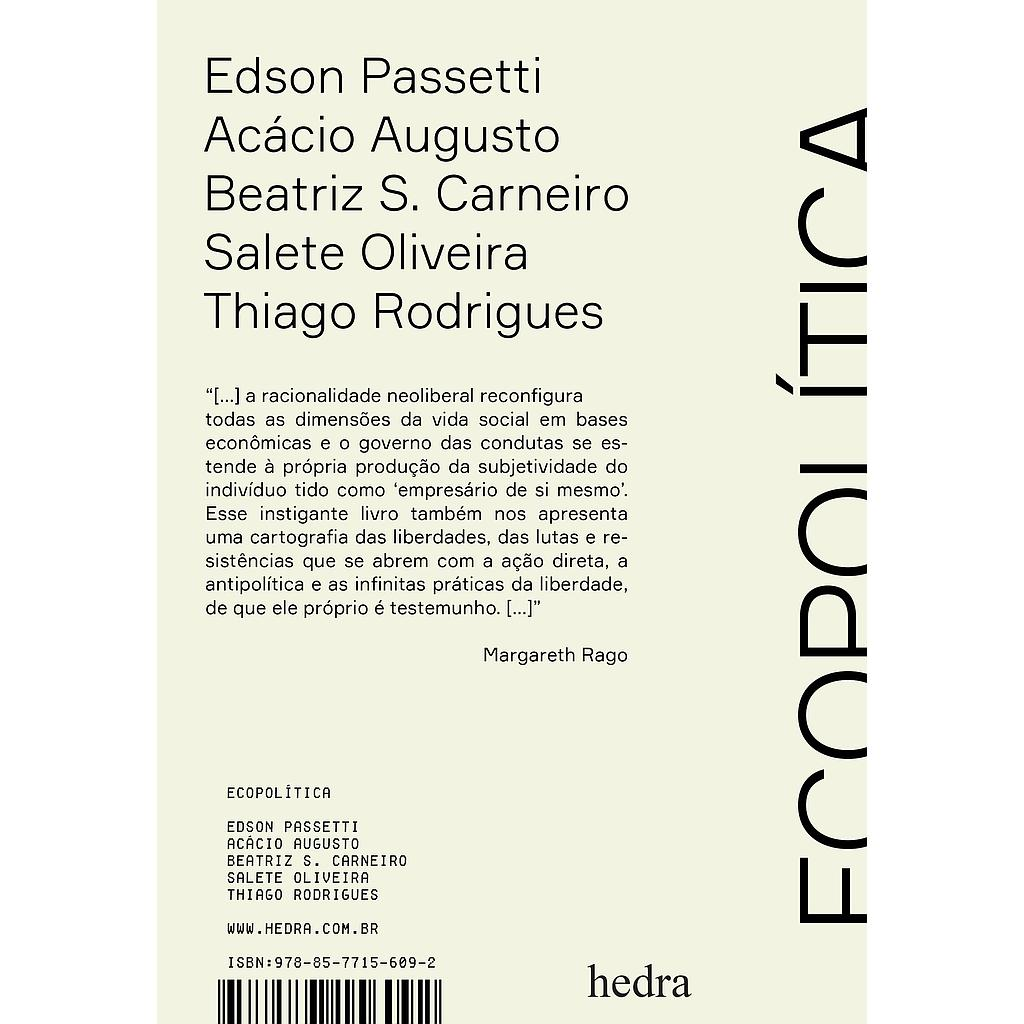
\includegraphics[width=92mm]{./grid/passetti.jpeg}
\end{center}

\hspace*{-7cm}\hrulefill\hspace*{-7cm}

\medskip

\noindent{}Na ecopolítica o alvo principal dos governos é o planeta, visando recuperar sua vida degradada e conservá"-lo de modo sustentável, em benefício das futuras gerações. Pressiona os regimes políticos para a democracia em sintonia com a racionalidade neoliberal. Pretende dar conta não só do governo da espécie humana, mas dos viventes na Terra.

Fruto de reuniões de estudiosos anarquistas, {\slsc{Ecopolítica}} mapeia a passagem da biopolítica --- o controle da vida analisado por Foucault --- para a ecopolítica, nova forma de governar que emerge pós"-\scalebox{.8}{II} Guerra Mundial e com as institucionalizações subsequentes, e se estende a todas as esferas do mundo natural. O grupo libertário Nu"-Sol percorre e analisa acontecimentos históricos e contemporâneos, e atravessa fluxos de poder para conclamar à criação de resistências libertárias e esquivas às globalizantes linhas de controle.

\vfill

\hspace*{-.4cm}\begin{minipage}[c]{.5\linewidth}
\small{
{\Formular{\textbf{
\hspace*{-.1cm}Título: Ecopolítica\\
Autor: Edson Passetti (org.)\\ 
ISBN: 978-85-7715-609-2\\
Páginas: 476\\
Formato: 16x23cm\\
Preço: R\$ 79,90\\
Editora: Hedra\\
Disponibilidade: Disponível
}}}}
\end{minipage}


\pagebreak


\hspace{.5cm}

\begin{center}
\hspace*{.5cm}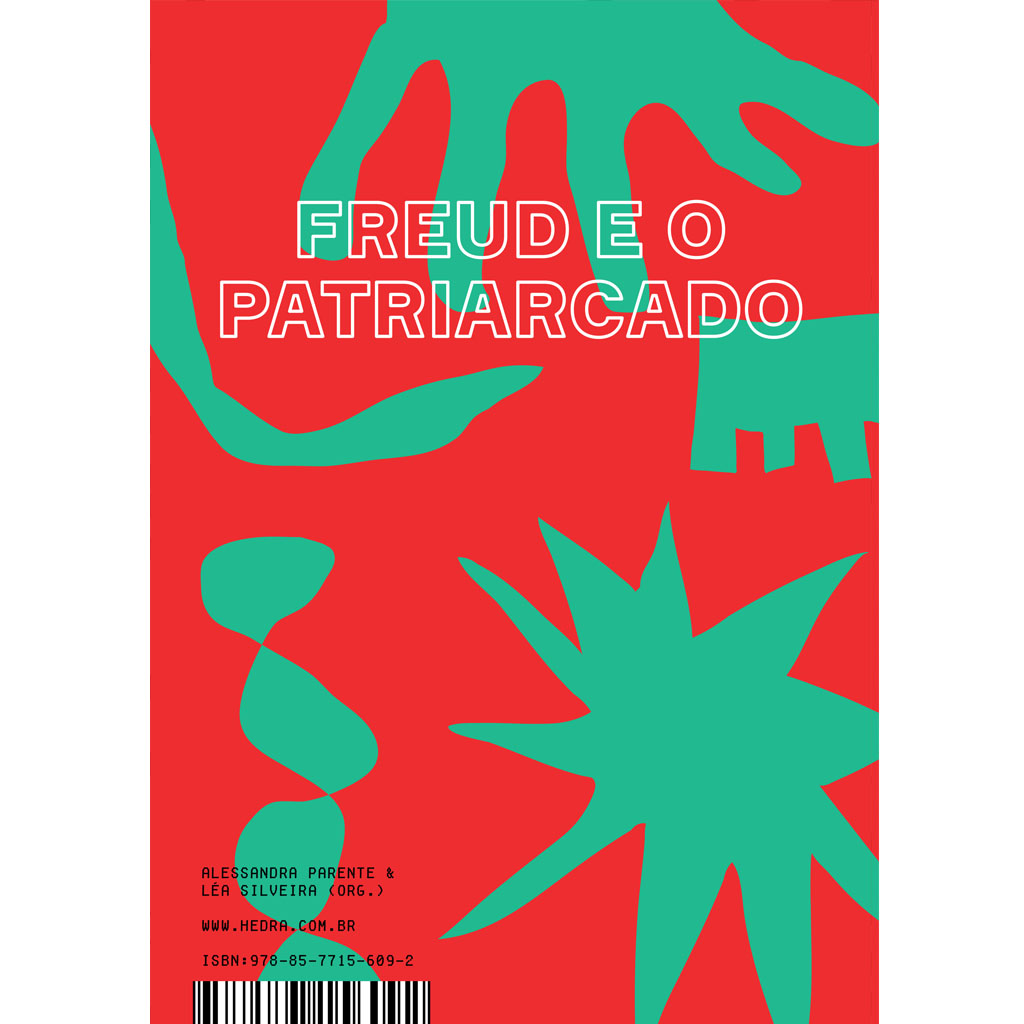
\includegraphics[width=92mm]{./grid/freud.jpg}
\end{center}

\hspace*{-7cm}\hrulefill\hspace*{-7cm}

\medskip

\noindent{}{\slsc{Freud e o patriarcado}} parte da constatação de que a teoria psicanalítica põe em jogo uma forma de conceber o psíquico --- ou a subjetividade --- como algo construído a partir de um modelo que assume uma equivalência generalizada entre cultura, civilização e masculinidade. Ao assumir esse parâmetro, a psicanálise coloca como modelo teórico algo que deveria ser explicado ao invés de tomado como dado.

A exploração e preservação dos modelos freudianos originários e em seus desdobramentos busca principalmente sua potência própria. Além dos apontamentos, nos próprios textos de Freud, de elementos que permitam vislumbrar modelos distintos. Repensando uma nova psicanálise urgente e alinhada ao progressivo empoderamento das mulheres e da luta feminista, o livro inclui diversas reflexões, que vão dos textos canônicos de Freud às novas abordagens de Oswald de Andrade, Deleuze e Guattari.

%\hspace{.5cm}
\vfill

\hspace*{-.4cm}\begin{minipage}[c]{.5\linewidth}
\small{
{\Formular{\textbf{
\hspace*{-.1cm}Título: Freud e o patriarcado\\
Autor: Alessandra Martins\\ Parente e Léa Silveira (org.)\\ 
ISBN: 978-85-7715-611-5\\
Páginas: 398\\
Formato: 16x23cm\\
Preço: R\$ 64,90\\
Editora: Hedra\\
Disponibilidade: Disponível
}}}}
\end{minipage}

\pagebreak

\hspace{.5cm}

\begin{center}
\hspace*{-2.5cm}\raisebox{6.8cm}{\rotatebox[origin=t]{90}{\huge\Formular{\textbf{Lançamento}}}}
\hspace*{2.5cm}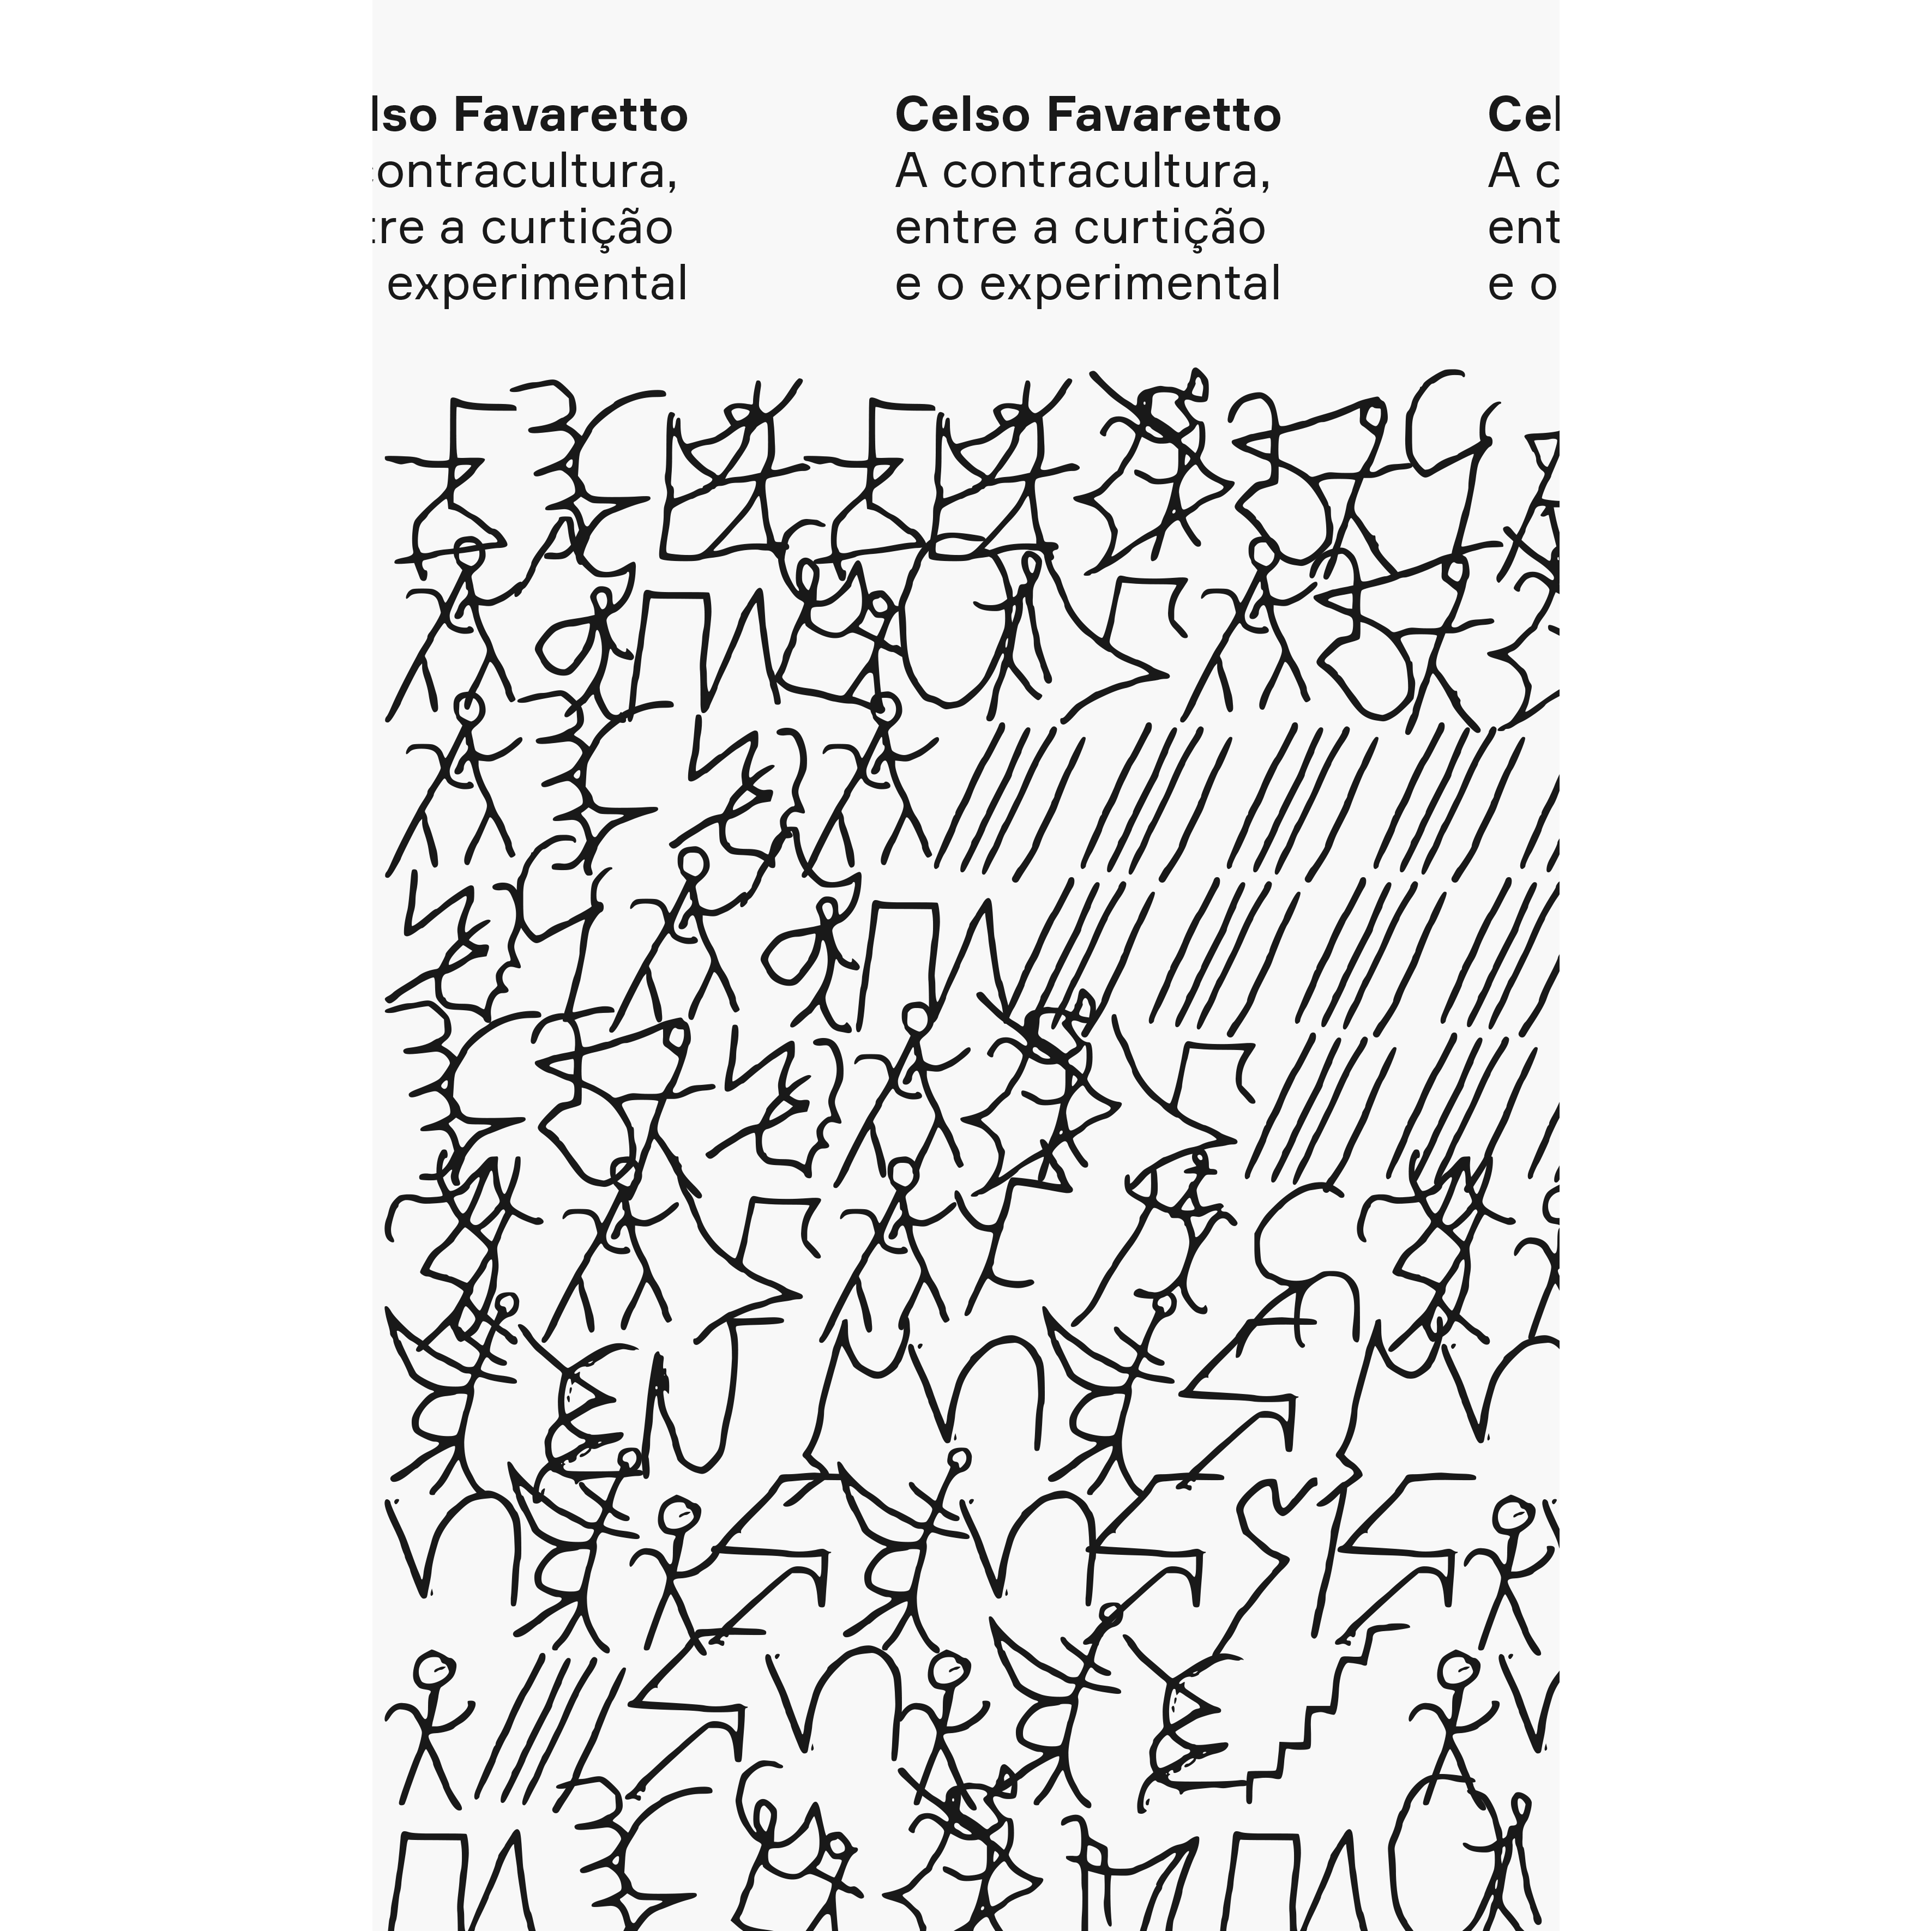
\includegraphics[width=92mm]{./grid/favaretto.png}
\end{center}

\hspace*{-7cm}\hrulefill\hspace*{-7cm}

\medskip

\noindent{}Neste livro o pesquisador e intelectual Celso Favaretto aborda as manifestações contraculturais que marcaram a produção artística brasileira entre os anos 60 e 70. Manifestava"-se então uma nova sensibilidade às margens da política oficial e da indústria cultural, expressa em experimentações artísticas com diversas possibilidades abertas pelo tropicalismo. Longe de um suposto “vazio cultural”, a contracultura nas variadas expressões definiu atitudes, comportamentos, gestos exemplares, experimentações de grande vitalidade. Inclusive, em alguns casos, a resistência às limitações da cultura oficial e à repressão da ditadura.

Composto por três ensaios, são revisitados no livro importantes personalidades e eventos da cultura brasileira --- como Caetano Veloso, Waly Salomão, Glauber Rocha, Zé Celso e o Teatro Oficina, Augusto Boal, Antonio Callado, José Agrippino de Paula, Hélio Oiticica --- sincrônicos aos desdobramentos políticos e sociais implicados pelo Golpe Civil"-Militar.

\vfill

\hspace*{-.4cm}\begin{minipage}[c]{.5\linewidth}
\small{
{\Formular{\textbf{
\hspace*{-.1cm}Título: A contracultura, entre\\ a curtição e o experimental\\
Autor: Celso Favaretto\\ 
ISBN: 978-65-8109-703-5\\
Páginas: 142\\
Formato: 11x18cm\\
Preço: R\$ 40,00\\
Editora: Hedra \& n-1\\
Disponibilidade: Disponível
}}}}
\end{minipage}

\pagebreak

\hspace{.5cm}

\begin{center}
\hspace*{.5cm}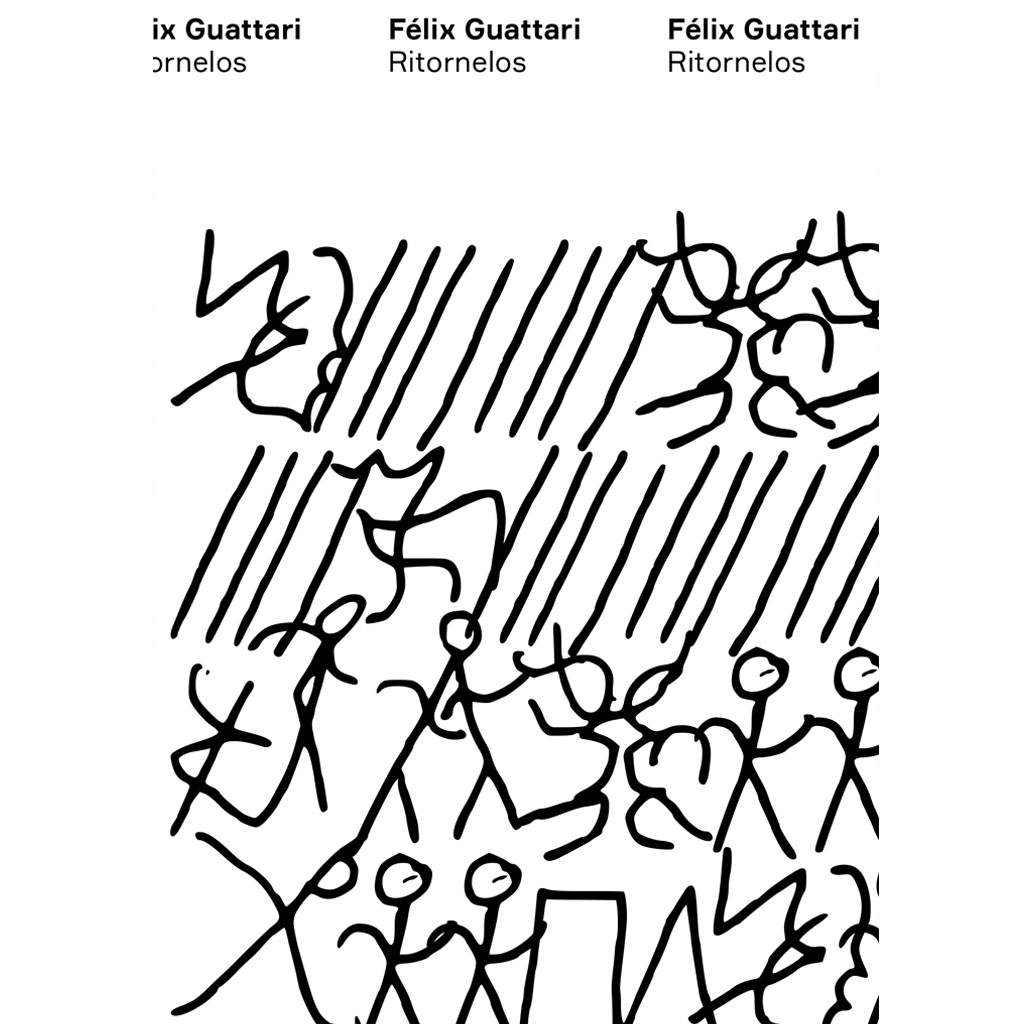
\includegraphics[width=92mm]{./grid/guattari.jpg}
\end{center}

\hspace*{-7cm}\hrulefill\hspace*{-7cm}

\medskip

\noindent{}Livro póstumo do pensador e psicanalista francês Félix Guattari, {\slsc{Ritornelos}} é uma obra inclassificável. Misto de poesia, relatos autobiográficos, {\slsc{frames}} do cotidiano, toda potência da escrita esquiza irrompe nessas páginas de alta voltagem poética e imagética. Além de arguto intelectual, Guattari aparece em {\slsc{Ritornelos}} enquanto poeta sensível aos instantâneos e surreais quadros da vida.

Ao longo de suas páginas, vemos a fluidez com que a escrita de Guattari escorre sobre a superfície da vida, penetra em suas estruturas fragmentadas e as transporta ao seu revés. Através desse torvelinho de imagens decompostas o livro leva o leitor a percorrer o universo único do filósofo: cenas de amor e intimidade, de amizades, captadas nas ruas e praças parisienses, suas referências literárias e cinematográficas, quase em um mapeamento afetivo e cartográfico do autor de {\slsc{O anti-Édipo}}. Publicado somente nos anos 2000 na França, é a primeira vez que o livro é traduzido e editado no Brasil, em trabalho minucioso de tradutor"-ourives para acompanhar todas as nuances, rupturas e labirintos do texto original.

\vfill

\hspace*{-.4cm}\begin{minipage}[c]{.5\linewidth}
\small{
{\Formular{\textbf{
\hspace*{-.1cm}Título: Ritornelos\\
Autor: Félix Guattari\\ 
ISBN: 978-65-8109-702-8\\
Páginas: 134\\
Formato: 11x18cm\\
Preço: R\$ 40,00\\
Editora: Hedra \& n-1\\
Disponibilidade: Disponível
}}}}
\end{minipage}

\pagebreak

\hspace{.5cm}

\begin{center}
\hspace*{-2.5cm}\raisebox{6.8cm}{\rotatebox[origin=t]{90}{\huge\Formular{\textbf{Lançamento}}}}
\hspace*{2.5cm}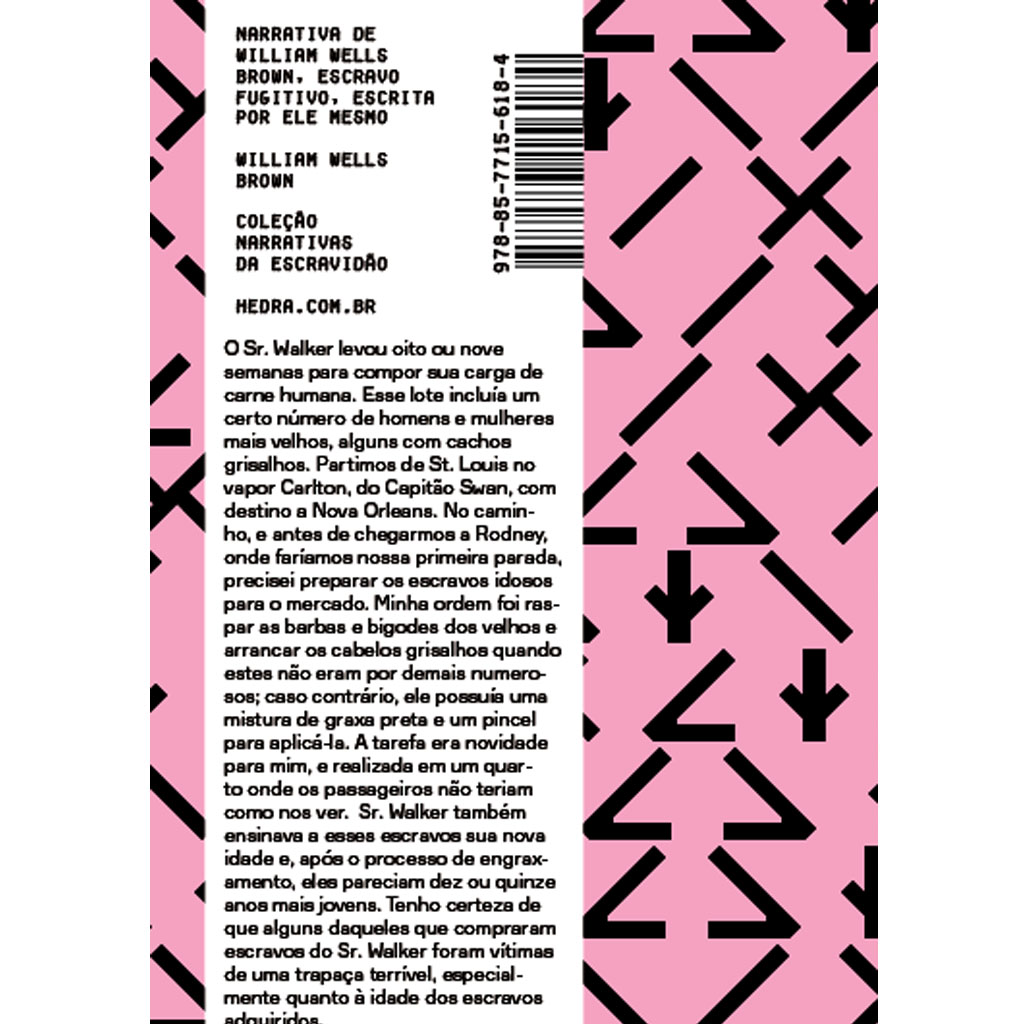
\includegraphics[width=92mm]{./grid/brown.jpg}
\end{center}

\hspace*{-7cm}\hrulefill\hspace*{-7cm}

\medskip

\noindent{}William Wells Brown (1814--1884) foi um abolicionista, romancista, dramaturgo e historiador afro"-americano. Nascido escravo, fugiu para a liberdade aos 20 anos de idade e, aos 33, publicou essa narrativa. Aqui conta a história de sua vida nos estados do Kentucky e Missouri, onde trabalhou como aprendiz em um jornal, transportando escravos para a venda em Nova Orleans e em diversas outras atividades. Descreve os horrores da escravidão, o tráfico interno de escravos nos \scalebox{.8}{EUA} e a relação de Brown com seus donos e familiares.

O autor, no entanto, não hesita em revelar seus vícios e defeitos, destacando assim a individualidade que se desenvolveu sob uma instituição totalizante e desumanizadora, que via em homens e mulheres apenas braços para a lavoura e ventres para uma nova geração de cativos. A {\slsc{Narrativa de William Wells Brown}} é uma crítica à ganância e à hipocrisia religiosa, ao preconceito e à violência, mas, acima de tudo, é uma proclamação da humanidade do seu autor e de todos que sofreram ao seu lado.

%\hspace{.5cm}
\vfill

\hspace*{-.4cm}\begin{minipage}[c]{.5\linewidth}
\small{
{\Formular{\textbf{
\hspace*{-.1cm}Título: Narrativa de William Wells\\ Brown, escravo fugitivo\\
Autor: William Wells Brown\\ 
ISBN: 978-85-7715-618-4\\
Páginas: 140\\
Formato: 14x21cm\\
Preço: R\$ 39,90\\
Editora: Hedra\\
Disponibilidade: Disponível
}}}}
\end{minipage}

\pagebreak

\hspace{.5cm}

\begin{center}
\hspace*{.5cm}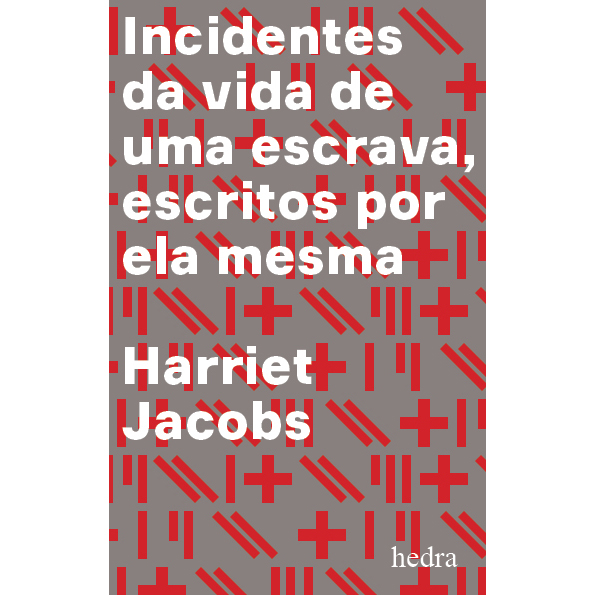
\includegraphics[width=92mm]{./grid/jacobs.jpg}
\end{center}

\hspace*{-7cm}\hrulefill\hspace*{-7cm}

\medskip

\noindent{}Nascida na Carolina do Norte por volta do outono de 1813, Harriet Ann Jacobs viveu a tragédia do cativeiro até principiar uma vida em fuga que terminou por levá"-la ao Norte em 1842. Foi de Boston que Jacobs pôde produzir {\slsc{Incidentes da vida de uma escrava}} que, sem deixar de se inserir no {\slsc{corpus}} dos relatos da escravidão norte"-americana, guarda uma singularidade: é pioneiro e inspirador das autobiografias femininas, e joga luz nos horrores que eram partilhados apenas entre as mulheres.

“A escravidão é terrível para os homens”, escreve a autora, “mas é muito mais terrível para as mulheres”. Jacobs convive, antes e depois da fuga, com o perverso sistema de assédio e coação sexual contra o qual as escravas procuravam lutar. Transmitindo brilhantemente uma vida em prosa crua e seca, {\slsc{Incidentes da vida de uma escrava}} adiciona camadas de complexidade ao horror da escravatura.

%\hspace{.5cm}
\vfill

\hspace*{-.4cm}\begin{minipage}[c]{.5\linewidth}
\small{
{\Formular{\textbf{
\hspace*{-.1cm}Título: Incidentes da vida de uma\\ escrava, escritos por ela mesma\\
Autor: Harriet Jacobs\\ 
ISBN: 978-85-7715-617-7\\
Páginas: 404\\
Formato: 14x21cm\\
Preço: R\$ 49,90\\
Editora: Hedra\\
Disponibilidade: Disponível
}}}}
\end{minipage}


\pagebreak

\hspace{.5cm}

\begin{center}
\hspace*{-2.5cm}\raisebox{6.8cm}{\rotatebox[origin=t]{90}{\huge\Formular{\textbf{Lançamento}}}}
\hspace*{2.5cm}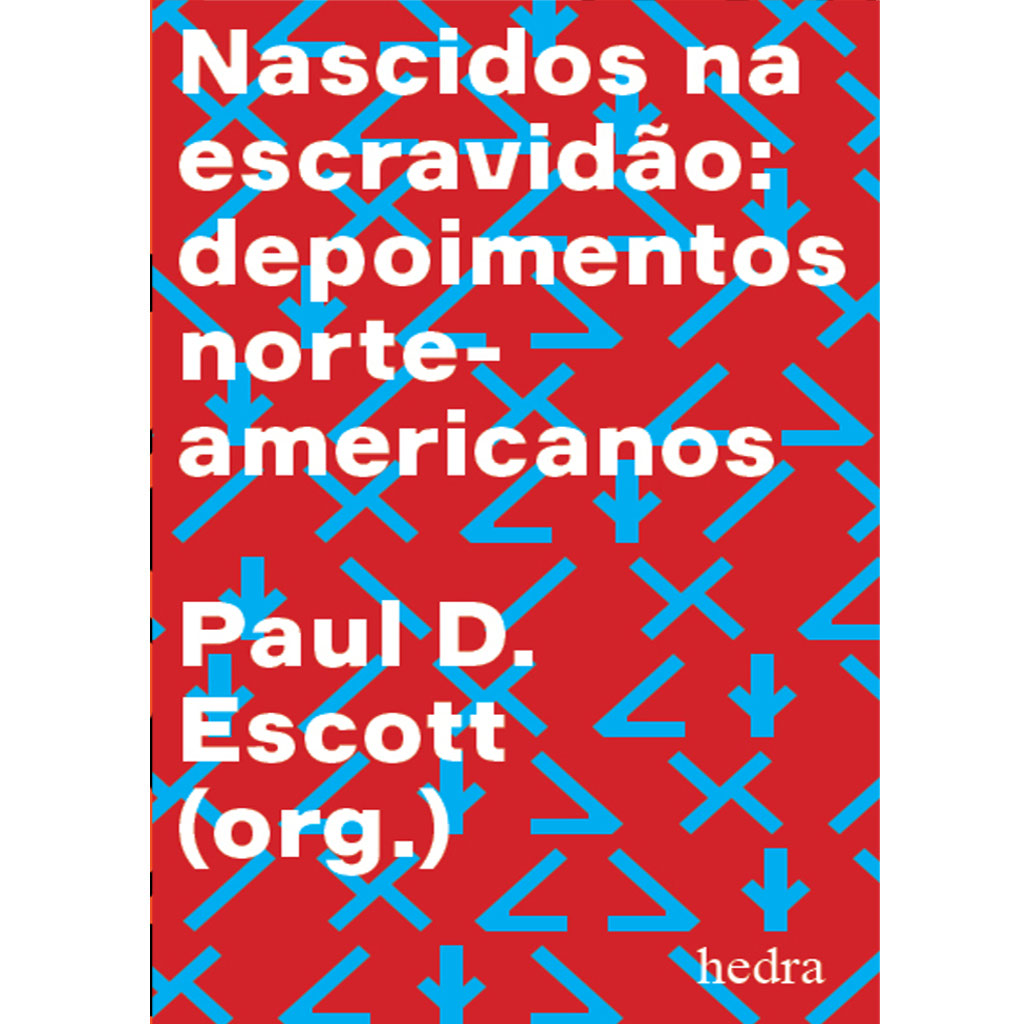
\includegraphics[width=92mm]{./grid/wpa.jpg}
\end{center}

\hspace*{-7cm}\hrulefill\hspace*{-7cm}

\medskip

\noindent{}Inéditas no país, a edição reune narrativas de 204 ex"-escravizados norte"-americanos sobre temas centrais da escravidão nas Américas: cultura negra, resistência, violência, relações familiares durante a escravidão, trabalho, emancipação --- organizadas por Paul D. Escott, historiador e professor da Wake Forest University.

Coletadas através do Projeto Federal de Escritores (\scalebox{.8}{FWP}), pertencente ao órgão Administração do Progresso no Trabalho (\scalebox{.8}{WPA}), criado na esteira da Crise de 1929 para garantir a renda de escritores desempregados, as narrativas revelam a memória das milhares de pessoas sobreviventes ao trauma da escravidão. Ao todo, o Projeto Federal de Escritores salvou 2400 narrativas, aproximações de dentro, em perspectiva única, do que foi o escravismo sulista norte"-americano, que às vésperas da abolição da escravatura contava com 4 milhões de escravizados em seus campos de trabalho.

%\hspace{.5cm}
\vfill

\hspace*{-.4cm}\begin{minipage}[c]{.5\linewidth}
\small{
{\Formular{\textbf{
\hspace*{-.1cm}Título: Nascidos na escravidão —\\ depoimentos norte"-americanos\\
Autor: Paul D. Escott (org.)\\ 
ISBN: 978-85-7715-619-1\\
Páginas: 354\\
Formato: 14x21cm\\
Preço: R\$ 49,90\\
Editora: Hedra\\
Disponibilidade: Disponível
}}}}
\end{minipage}

\pagebreak

\hspace{.5cm}

\begin{center}
\hspace*{.5cm}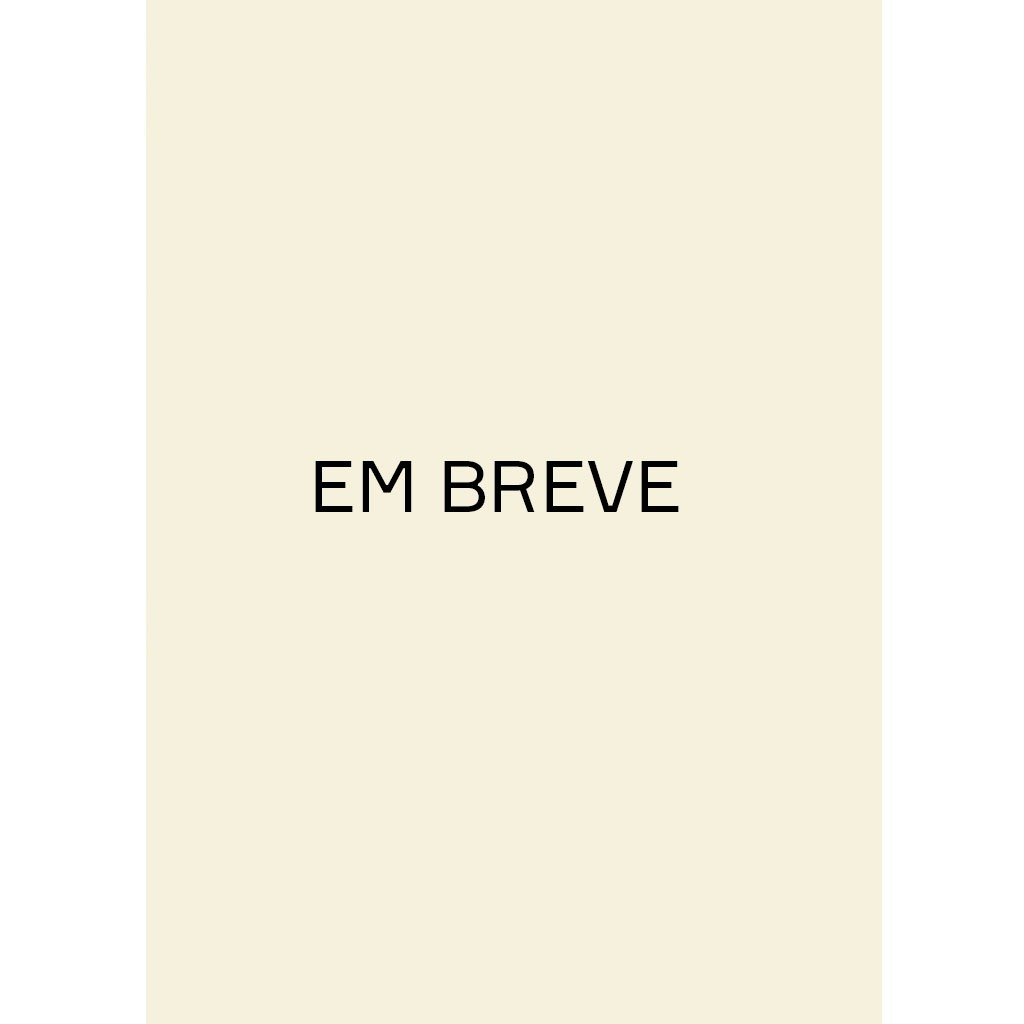
\includegraphics[width=92mm]{./grid/breve.jpeg}
\end{center}

\hspace*{-7cm}\hrulefill\hspace*{-7cm}

\medskip

\noindent{}A ascensão ao poder de uma direita radicalizada, nova sobretudo nos métodos de ação e no uso eficiente das tecnologias modernas, impõe uma reflexão de ordem tática: o que é, hoje, o antifascismo? Como a convulsão social pode organizar"-se contra o controle imposto por polícias ultraviolentas?
Se por um lado governantes como Jair Bolsonaro ou Donald Trump dispõem de amplo arsenal fático e bélico, a explosão recente de protestos pelo mundo aponta para uma janela de ação, em que a revolta popular também se radicaliza e, literalmente, coloca nações inteiras em chamas.

E é na esteira desse momento fundamental que é estruturado {\slsc{Antifa: modo de usar}}. A publicação reúne ensaios, textos e entrevistas do historiador americano Mark Bray, especialista no movimento antifascista e uma das principais vozes do momento de luta. Além de textos de Acácio Augusto --- organizador do volume, cientista social e pesquisador em estudos libertários do grupo Nu-Sol --- compondo um material urgente e essencial para nosso tempo.

\vfill

\hspace*{-.4cm}\begin{minipage}[c]{.5\linewidth}
\small{
{\Formular{\textbf{
\hspace*{-.1cm}Título: Antifa: modo de usar\\
Autor: Mark Bray\\
Organizador: Acácio Augusto\\ 
ISBN: 978-85-7715-652-8\\
Páginas: ???\\
Formato: 12,7x19,1cm\\
Preço: R\$ ????\\
Editora: Hedra \& Circuito\\
Disponibilidade: 17/07/2020
}}}}
\end{minipage}

\pagebreak

\hspace{.5cm}

\begin{center}
\hspace*{-2.5cm}\raisebox{6.8cm}{\rotatebox[origin=t]{90}{\huge\Formular{\textbf{Lançamento}}}}
\hspace*{2.5cm}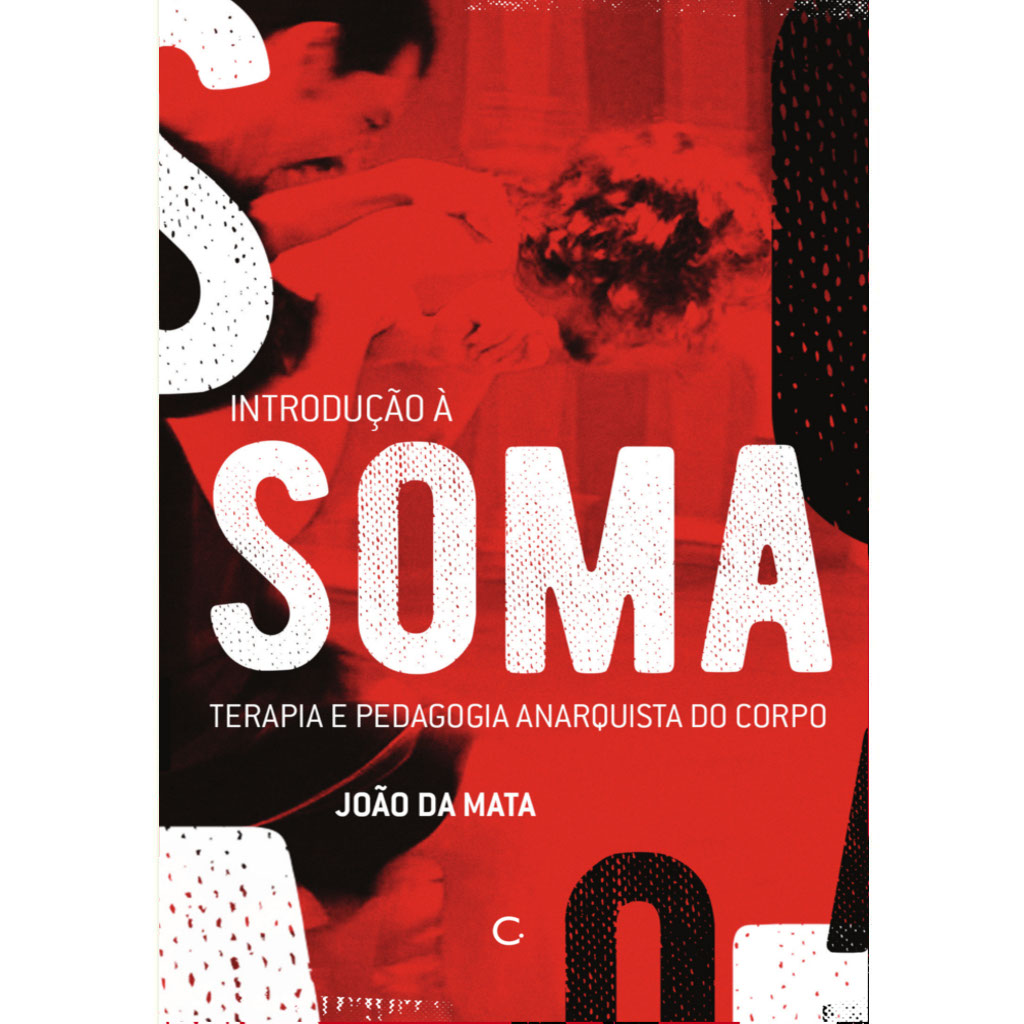
\includegraphics[width=92mm]{./grid/soma.jpg}
\end{center}

\hspace*{-7cm}\hrulefill\hspace*{-7cm}

\medskip

\noindent{}{\slsc{Introdução à Soma: terapia e pedagogia anarquista do corpo}} trata de um processo terapêutico corporal realizado em grupo, que busca no pensamento anarquista uma crítica às mais variadas formas de poder impregnadas no comportamento individual e nas relações sociais. O grupo de terapia funciona como um micro"-laboratório social, no qual se desenvolve uma análise libertária do comportamento de cada um a partir da relação junto ao outro.

Daí sua originalidade: terapia como criação e afirmação de si, em que a construção das práticas de liberdade é o antídoto para combater os conflitos gerados pelas relações sociais hierarquizadas. A somaterapia ou apenas Soma é um processo terapêutico"-pedagógico, realizado em grupo e com ênfase na articulação entre o trabalho corporal e o uso da linguagem verbal. Foi criada no Brasil pelo escritor e terapeuta Roberto Freire, a partir da obra de Wilhelm Reich e sua pesquisa sobre corpo e emoção.

\vfill

\hspace*{-.4cm}\begin{minipage}[c]{.5\linewidth}
\small{
{\Formular{\textbf{
\hspace*{-.1cm}Título: Introdução à Soma — terapia\\ e pedagogia anarquista do corpo\\
Autor: João da Mata\\ 
ISBN: 978-85-9582-055-5\\
Páginas: 106\\
Formato: 12,7x19,1cm\\
Preço: R\$ 42,90\\
Editora: Hedra \& Circuito\\
Disponibilidade: 17/07/2020
}}}}
\end{minipage}

\pagebreak

\hspace{.5cm}

\begin{center}
\hspace*{.5cm}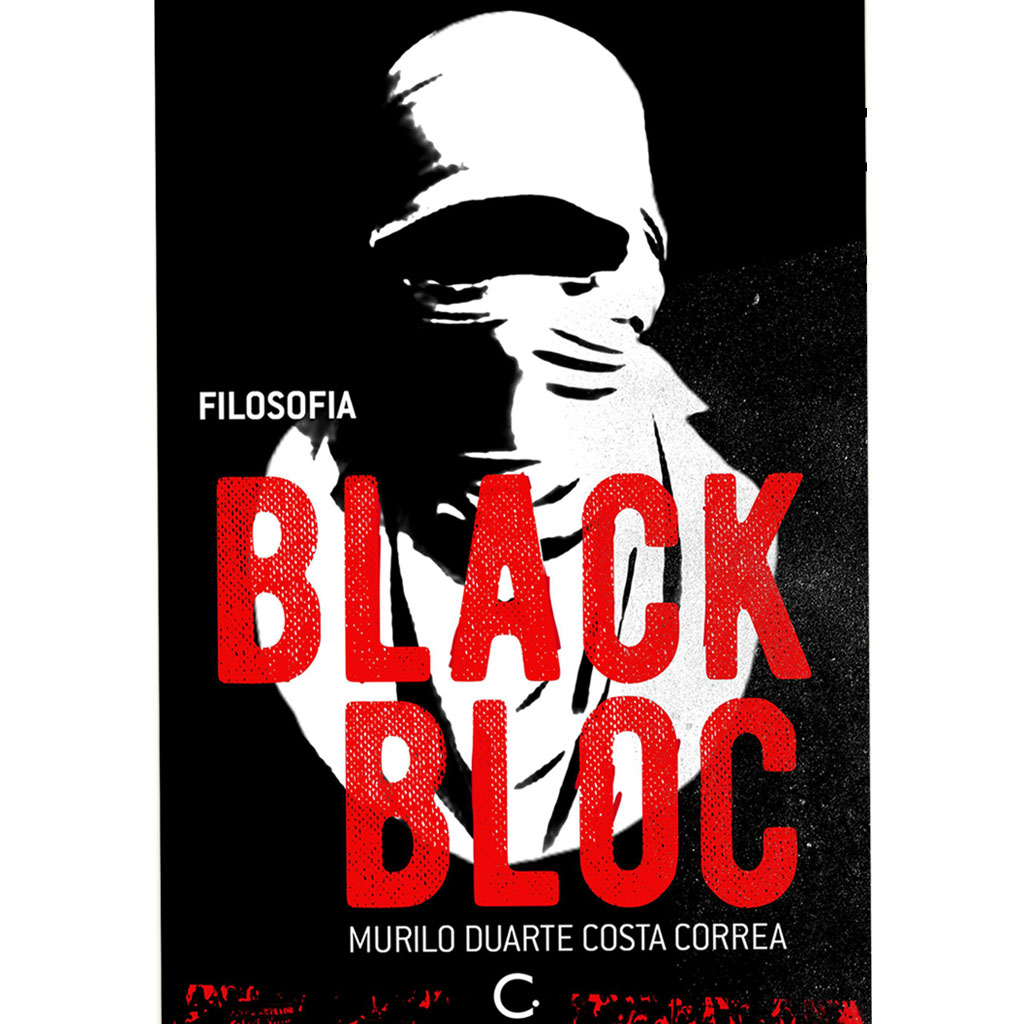
\includegraphics[width=92mm]{./grid/black.jpg}
\end{center}

\hspace*{-7cm}\hrulefill\hspace*{-7cm}

\medskip

\noindent{}Em junho de 2013, data da maior erupção social das últimas décadas, o movimento {\slsc{Black Bloc}} ganhou os holofotes como nova prática de luta e manifestação. Analistas à direita e à esquerda foram forçados a tentar compreender o movimento, normalmente municiando um repertório conceitual incompatível com os significados do {\slsc{Black Bloc}}, sem entendê"-lo em seus próprios termos.

Procurando suprir essa carência surge o {\slsc{Filosofia Black Bloc}}, que concebe e mobiliza um arcabouço teórico que permita abordar o movimento {\slsc{Black Bloc}} como fenômeno: produzir, no pensamento, uma filosofia {\slsc{Black Bloc}}. Não cessamos de ler Junho sob o ponto de vista de Brasília, dos palácios de governo, dos partidos recusados pelas multidões, da surpresa e da inércia dos poderes constituídos, da decadência da representação formal, das classes cerradas para o social. Pensar Junho nesses termos torna"-se então “capturar e destruir” sua potência específica. Não é por acaso que boa parte das interpretações de intelectuais se parece tanto com os discursos da grande imprensa que vimos circular.

%\hspace{.5cm}
\vfill

\hspace*{-.4cm}\begin{minipage}[c]{.5\linewidth}
\small{
{\Formular{\textbf{
\hspace*{-.1cm}Título: Filosofia Black bloc\\
Autor: Murilo Duarte Costa Correa\\ 
ISBN: 978-85-9582-056-2\\
Páginas: 166\\
Formato: 12,7x19,1cm\\
Preço: R\$ 46,90\\
Editora: Hedra \& Circuito\\
Disponibilidade: 17/07/2020
}}}}
\end{minipage}

\pagebreak

\hspace{.5cm}

\begin{center}
\hspace*{-2.5cm}\raisebox{6.8cm}{\rotatebox[origin=t]{90}{\huge\Formular{\textbf{Lançamento}}}}
\hspace*{2.5cm}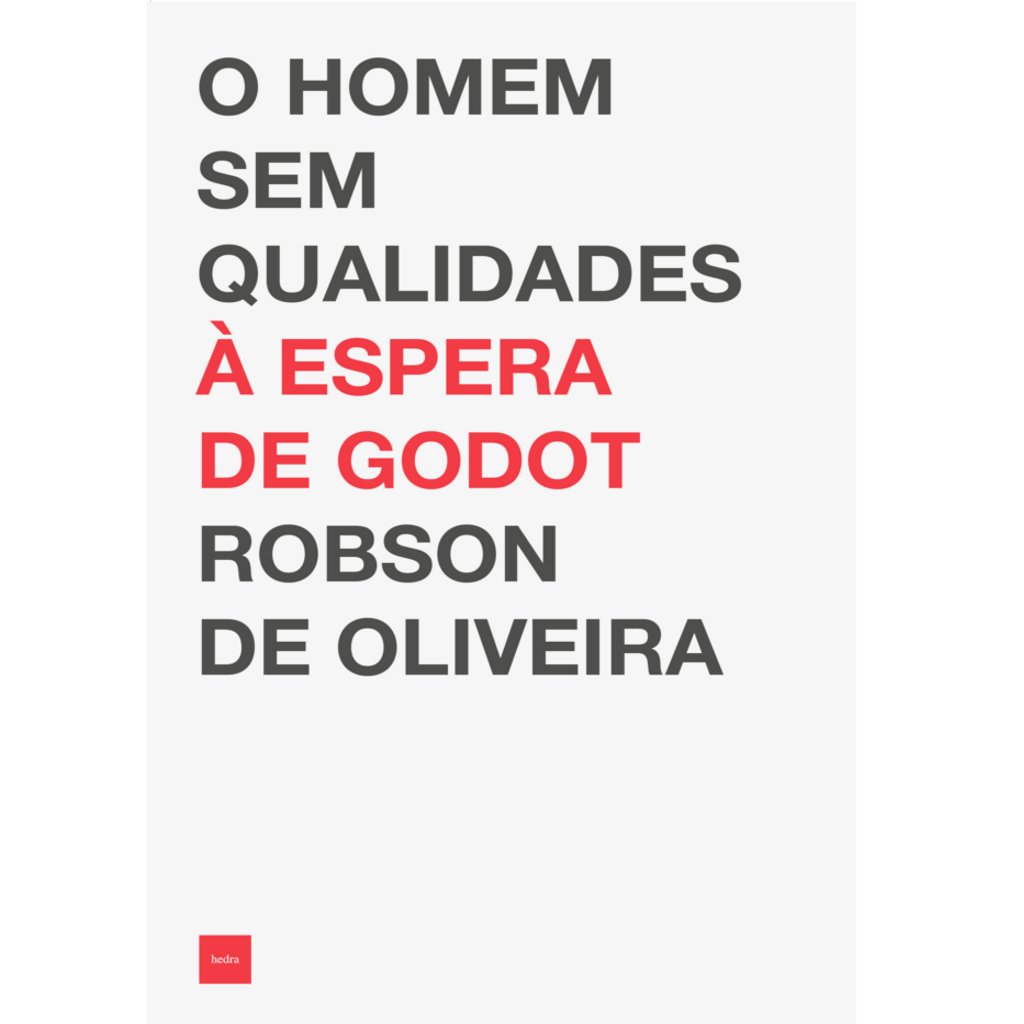
\includegraphics[width=92mm]{./grid/robson.jpg}
\end{center}

\hspace*{-7cm}\hrulefill\hspace*{-7cm}

\medskip

\noindent{}De forma ousada e criativa, {\slsc{O homem sem qualidades à espera de Godot}} procura a interdisciplinaridade dos saberes sobre o ser humano. Molière, Musil, Beckett, Caio Prado, Adorno, Marcuse e Robert Kurz, entre outros, são apresentados como “boa vizinhança” para essa reflexão. 

A grande questão aqui colocada é a de saber em que momento e através de quais mecanismos sociais e econômicos enaltecemos a mercadoria na nossa lógica de vida. Tornar"-se mercadoria do mundo representa tornar"-se vazio da própria subjetividade, onde reinam as leis mercantis que dominam nossos atos mais banais. 

%\hspace{.5cm}
\vfill

\hspace*{-.4cm}\begin{minipage}[c]{.5\linewidth}
\small{
{\Formular{\textbf{
\hspace*{-.1cm}Título: O homem sem qualidades\\ à espera de Godot\\
Autor: Robson de Oliveira\\ 
ISBN: 978-85-7715-614-6\\
Páginas: 510\\
Formato: 13,3x21cm\\
Preço: R\$ 44,90\\
Editora: Hedra\\
Disponibilidade: 31/07/2020
}}}}
\end{minipage}

\pagebreak


\hspace{.5cm}

\begin{center}
\hspace*{.5cm}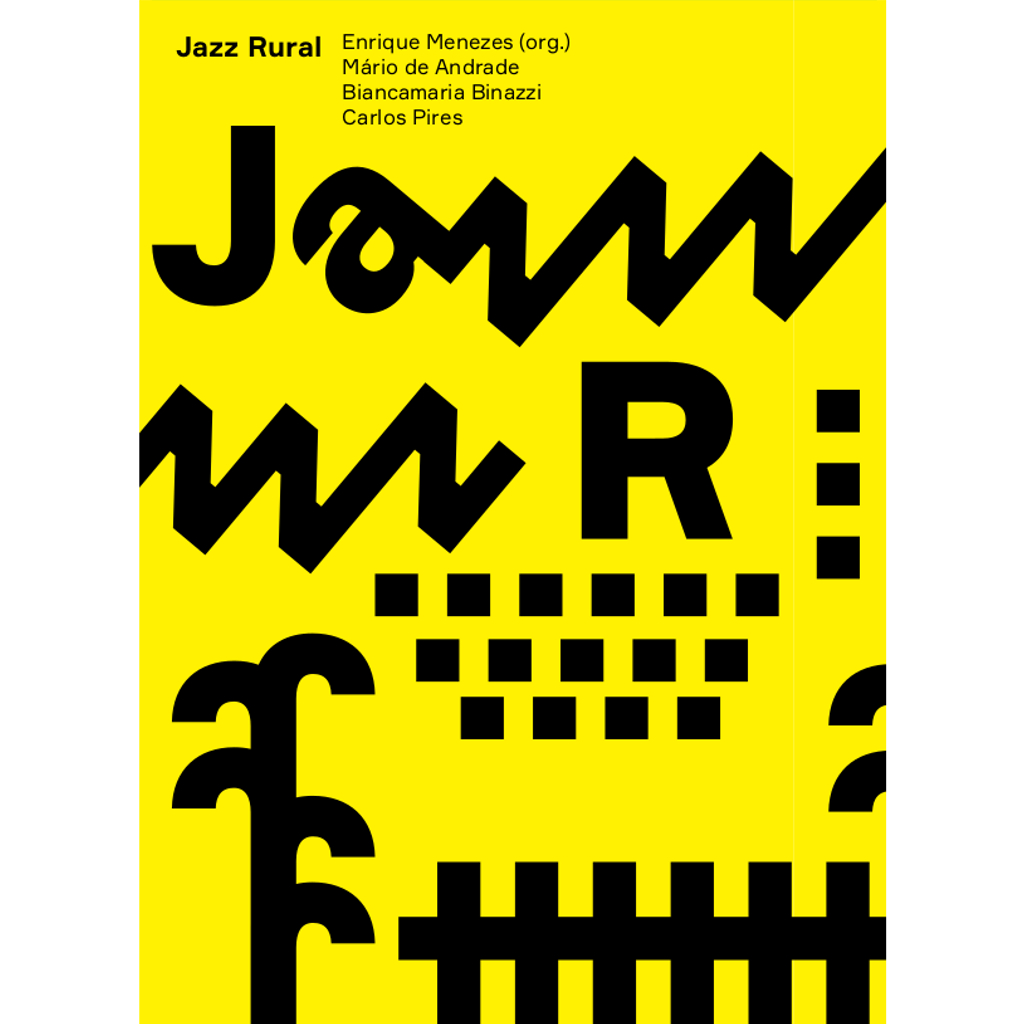
\includegraphics[width=92mm]{./grid/jazz.jpg}
\end{center}

\hspace*{-7cm}\hrulefill\hspace*{-7cm}

\medskip

\noindent{}{\slsc{Jazz Rural}} reúne dois textos de Mário de Andrade e gravações musicais de campo comandadas por ele na década de 1930 no interior de São Paulo --- cinco gravações feitas entre 1937--1942, disponíveis através de um \scalebox{.8}{QR} code na quarta capa. Mário foi o primeiro diretor do Departamento de Cultura de São Paulo, e projetou um rico conjunto de ações para as instituições públicas culturais --- entre elas a Discoteca Pública, com um selo para gravação de discos.

E não apenas os discos, mas filmagens, fotografias e anotações feitas pela equipe do Departamento são o laboratório da famosa “missão de pesquisas folclóricas”, realizada depois em estados do norte e nordeste. Desses escritos e músicas paulistas deriva a reflexão contemporânea proposta pelo grupo Jazz Rural, com textos críticos e composições experimentais inspiradas na pesquisa musical modernista de Mário em São Paulo.

\vfill

\hspace*{-.4cm}\begin{minipage}[c]{.5\linewidth}
\small{
{\Formular{\textbf{
\hspace*{-.1cm}Título: Jazz Rural\\
Autor: Mário de Andrade\\ e Enrique Menezes (org.)\\ 
ISBN: 978-85-7715-613-9\\
Páginas: 152\\
Formato: 13,3x21cm\\
Preço: R\$ ????\\
Editora: Hedra\\
Disponibilidade: 31/07/2020
}}}}
\end{minipage}

\pagebreak

\hspace{.5cm}

\begin{center}
\hspace*{-2.5cm}\raisebox{6.8cm}{\rotatebox[origin=t]{90}{\huge\Formular{\textbf{Lançamento}}}}
\hspace*{2.5cm}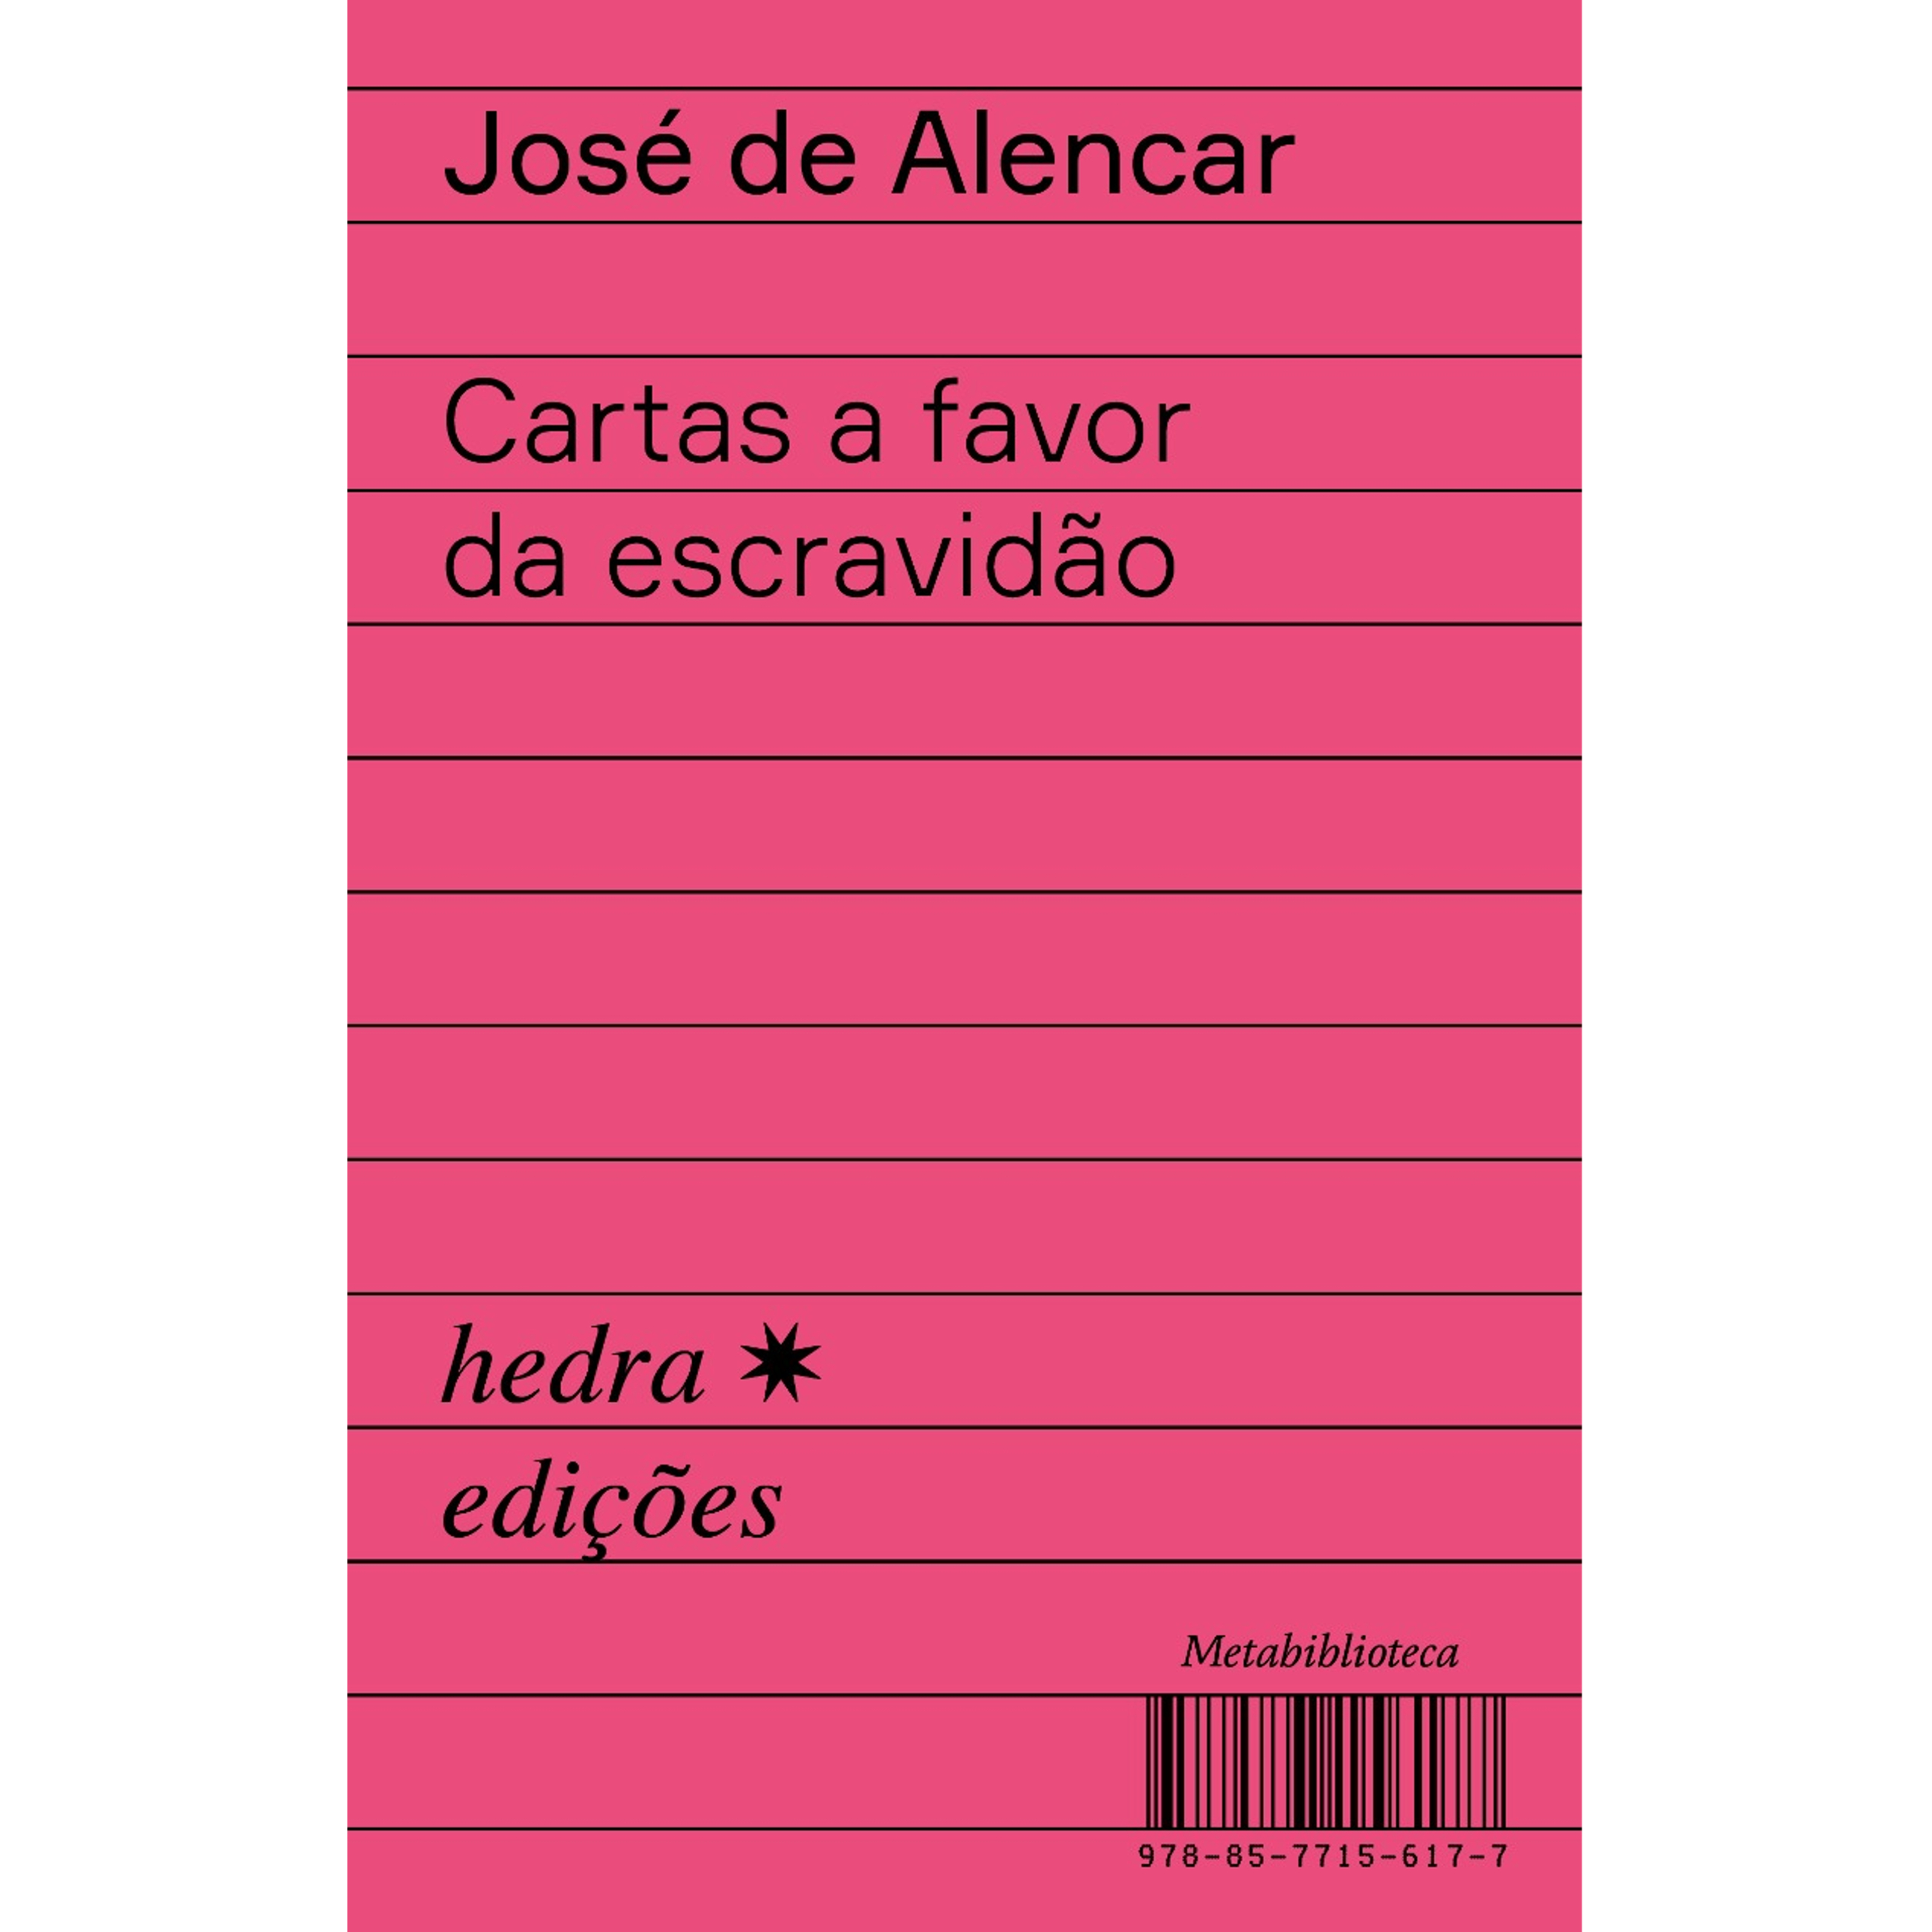
\includegraphics[width=92mm]{./grid/alencar.jpg}
\end{center}

\hspace*{-7cm}\hrulefill\hspace*{-7cm}

\medskip

\noindent{}José de Alencar, um dos autores mais lidos do século \scalebox{.8}{XIX}, aparece em {\slsc{Cartas a favor da escravidão}} com uma faceta menos conhecida: tentando demonstrar a D.~Pedro \scalebox{.8}{II} que a manutenção da escravatura servia melhor à nação do que seu fim --- onde expõe os principais traços argumentativos que justificam uma instituição hoje universalmente condenada. Pela primeira vez reeditadas desde o século \scalebox{.8}{XIX}, após terem sido expurgadas de sua obra, esses sete textos políticos foram publicados à época em franca oposição ao imperador, sob o título {\slsc{Ao imperador: novas cartas políticas de Erasmo}} (1867--1868).

Após a abolição nos Estados Unidos (1865), a escravidão brasileira vinha sofrendo intensa pressão internacional e doméstica. A presente publicação fornece um precioso material ao público interessado nos atuais debates sobre relações raciais no país, sendo incontornável para a nossa historiografia política e literária, bem como para o pensamento da história das relações raciais e escravidão no Brasil e no mundo.
%\hspace{.5cm}
\vfill

\hspace*{-.4cm}\begin{minipage}[c]{.5\linewidth}
\small{
{\Formular{\textbf{
\hspace*{-.1cm}Título: Cartas a favor da escravidão\\
Autor: José de Alencar\\ 
ISBN: 978-85-7715-640-5\\
Páginas: ????\\
Formato: 13,3x21cm\\
Preço: R\$ ???\\
Editora: Hedra\\
Disponibilidade: 31/07/2020
}}}}
\end{minipage}

\pagebreak

\hspace{.5cm}

\begin{center}
\hspace*{.5cm}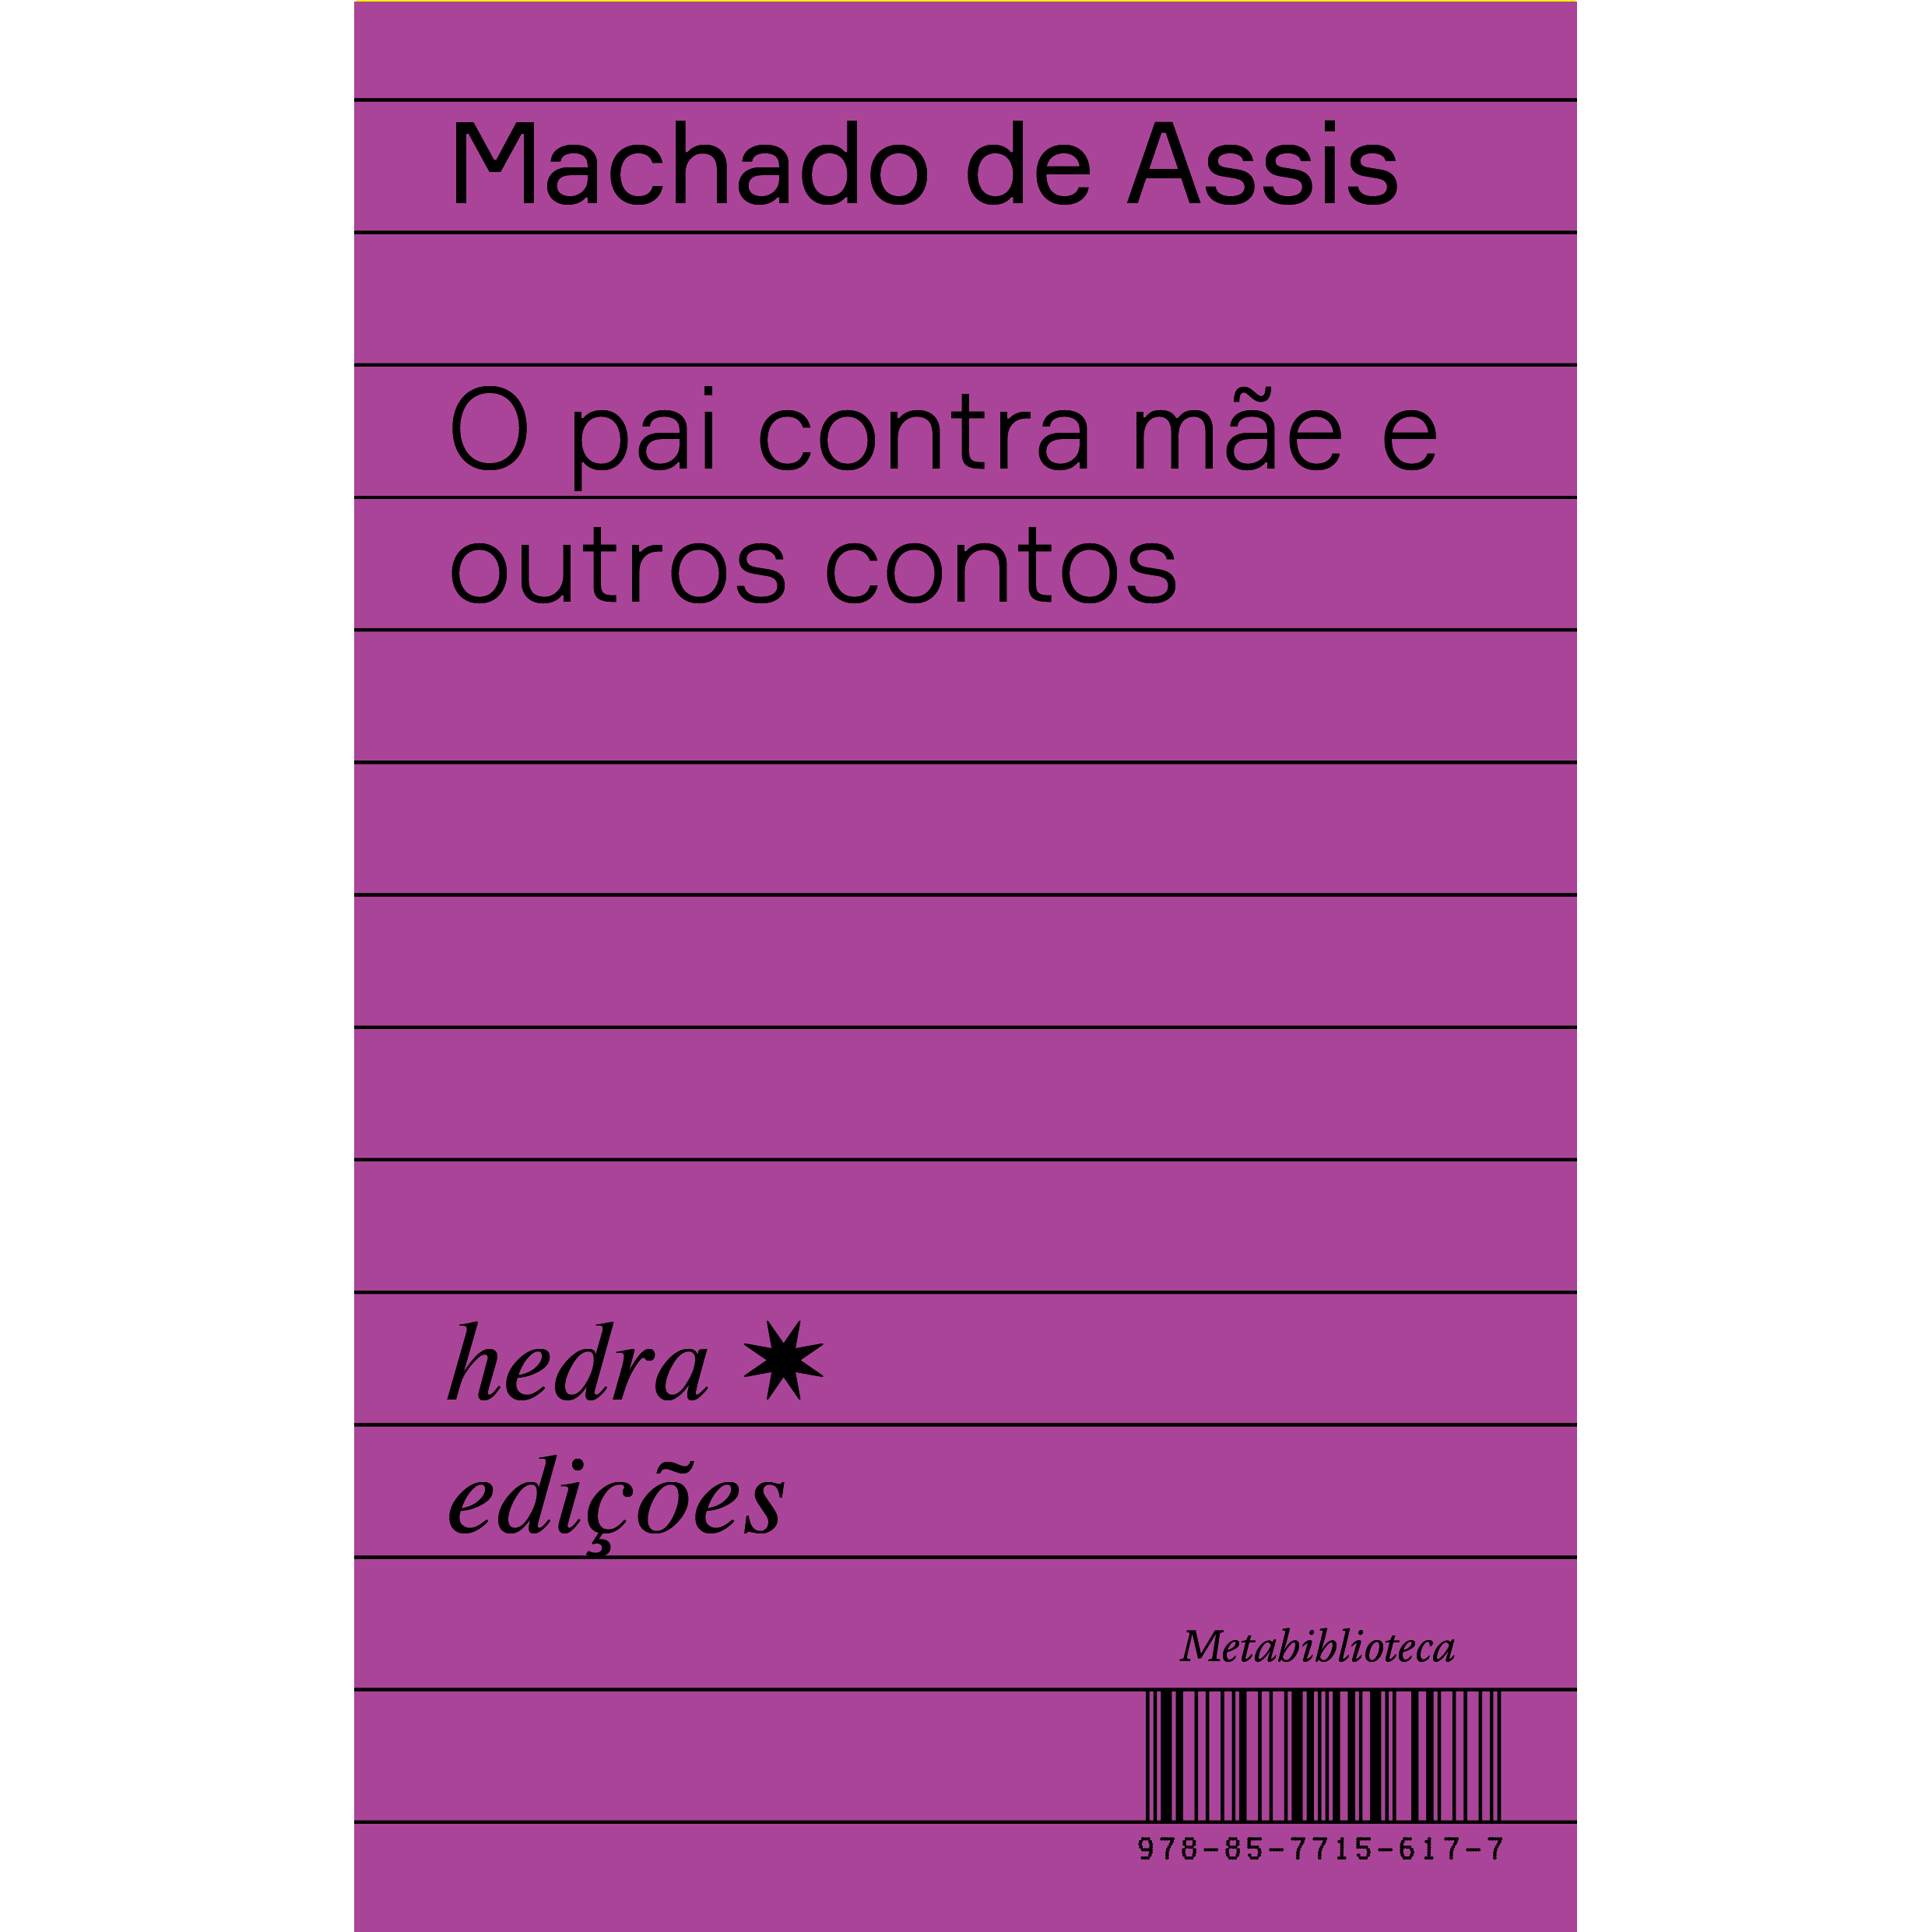
\includegraphics[width=92mm]{./grid/machad.jpg}
\end{center}

\hspace*{-7cm}\hrulefill\hspace*{-7cm}

\medskip

\noindent{}Como um obstetra que nos dá as boas"-vindas a este mundo com um tapa que nos faz chorar, o narrador machadiano de {\slsc{Pai contra mãe}} rasga o ventre de seu conto sentenciando que “a ordem social e humana nem sempre se alcança sem o grotesco, e alguma vez o cruel”. {\slsc{Pai contra mãe e outros contos}} é uma compilação de 33 narrativas breves do escritor carioca. Como na história que intitula o volume, as narrativas abordam os males e contradições de um Brasil que tenta se modernizar mas carrega seus arcaísmos herdados da colonização, como a escravidão e a política elitizada.

Machado de Assis é frequentemente considerado o maior escritor brasileiro de todos os tempos e em sua obra expõe, com prosa brilhante e ironia fina, a espinha dorsal das relações sociais da sociedade brasileira de seu tempo, da qual carregamos hoje muitas heranças. Em ambos os casos, os escritos de Machado, para além do incalculável valor literário, permanecem atuais como grandes reflexões acerca do Brasil do século \scalebox{.8}{XIX} e do atual.


\vfill

\hspace*{-.4cm}\begin{minipage}[c]{.5\linewidth}
\small{
{\Formular{\textbf{
\hspace*{-.1cm}Título: Pai contra mãe e outros contos\\
Autor: Machado de Assis\\ 
ISBN: 978-85-7715-628-3\\
Páginas: ????\\
Formato: 13,3x21cm\\
Preço: R\$ 50\\
Editora: Hedra\\
Disponibilidade: 31/07/2020
}}}}
\end{minipage}

\pagebreak

\begin{changemargin}
\hspace{.5cm}
\vspace*{1cm}
\enlargethispage{-\baselineskip}

\noindent{}{\LARGE{A velha novela do conto e do romance\\\noindent{}{\large\slsc{Existe um tipo intermediário entre romance e conto, a novela. E novela não é romance: mas como defini-la?}}}}

\medskip

\hfill{}\scalebox{.8}{LUIS DOLHNIKOFF}

\bigskip

Quais e quantos subgêneros comporta a prosa de ficção? Este texto aborda a questão em si, da forma mais abrangente e sintética que foi possível. ``Eu sei o que é o tempo, quando não tenho de defini"-lo, mas não sei, quando tenho''. Se, de um lado, estas famosas palavras de Santo Agostinho se aplicam a várias outras coisas além da coisa indefinível por excelência que é o tempo, por outro, se alguma coisa tem infinitas definições, tampouco tem uma definição precisa ou suficiente, como o amor. Mas coisas aparentemente muito mais simples também podem enfrentar a indefinição, ou a indefinibilidade. Por exemplo: o que é, afinal, uma novela?

No Brasil, em primeiro lugar, é uma forma popular de teledramaturgia. Portanto, sabemos o que é uma novela. Mas deixamos de saber, ou ao menos de saber com precisão, o que ela é quando se tenta aplicar o termo à literatura. Tudo se torna, então, cinza ou indefinido. Pois a novela, para os que defendem a existência de tal gênero narrativo, ocupa uma zona nebulosa entre o conto e o romance.

Parte do problema se origina na dupla nomeação. Enquanto romance vem da tradição das línguas românicas, ou neolatinas, e se refere a uma longa narrativa cavalheiresca (originalmente em versos), novela vem do próprio latim, de {\slsc{novus}}, novo, novidade, notícia. Assim, entre as principais línguas ocidentais, enquanto em francês romance é {\slsc{roman}}, em alemão, {\slsc{Roman}}, em italiano, {\slsc{romanzo}}, em espanhol e em inglês coexistem tanto a forma romance quanto novela --- ou {\slsc{novel}}. Se for este o caso --- e é este o caso ---, romance e novela são a mesma coisa. Ou deveriam ser. 

Mas se novela e romance são a mesma coisa, trata"-se apenas de um caso de sinonímia, como cão e cachorro, ou prédio e edifício. Haveria, afinal, apenas dois gêneros definíveis e definidos de prosa de ficção: conto e novela ou romance. Mas não é do que se trata. Pois toda a questão é a presumida existência de um terceiro tipo intermediário entre o romance e o conto, a novela. Então, novela não é romance. Mas se não é, como defini"-la? Como uma ``zona intermediária'' entre o conto e o romance.

O problema, no entanto, se mantém. Pois então o que diferenciaria a novela do conto longo, também dentro da ``zona intermediária'' entre o conto puro e o romance idem, e a novela do romance curto? Trocando em miúdos: se novela não é, afinal, um sinônimo ocioso de romance, e por isso mesmo nomeia a ``zona intermediária'', novela é o mesmo que conto longo ou que romance curto?

Há muitas tentativas de quantificar os gêneros: o conto, por exemplo, é uma narrativa com até 40 mil palavras. Enquanto o romance teria entre 41 mil e 100 mil ou mais palavras. Neste caso, um conto longo seria, de fato, indistinguível de um romance curto, pois o conto longo, alongando"-se um pouco de sua faixa padrão, teria talvez 41 mil palavras, enquanto um romance curto, encurtando outro tanto a sua faixa padrão, talvez tivesse 40 mil. Duas conclusões: conto e romance são a mesma coisa (ao menos seriam a mesma coisa o conto longo e o romance curto), e novela nomeia tanto o conto longo quanto o romance curto\ldots{} Se isto não parece fazer sentido, é porque não faz sentido.

Na tradição anglo"-saxã, e mais particularmente, norte"-americana, existem 6 subdivisões do gênero: {\slsc{flash fiction}}, {\slsc{short story}}, {\slsc{novelette}}, {\slsc{novella}}, {\slsc{novel}} e {\slsc{epic novel}}. Todas se definem pelo número de palavras: 100 a 2500, 2000 a 7500, 7500 a 15000, 15000 a 40000, 41000 a 100000, 101000 a 200000 palavras, respectivamente. Desconheço, em português, a expressão ``romance épico'', a não ser como um clichê eventualmente usado em material de divulgação editorial. ``Ficção"-relâmpago'' talvez seja o equivalente a microconto. Neste caso, voltamos, inevitavelmente, à palavra conto. E o que seria uma noveleta? Novelinha? Pequena novela? Novela curta? O que, então, diferenciaria, mais uma vez, uma novela curta de um conto longo? Há muito de mercadológico, além de certo afã sistematizador quantitativo, nesse divisionismo. Para piorar, ele não é o bastante.

A coisa começa, afinal, a ficar menos obscura. Porque se pode definir o conto e o romance tanto em termos quantitativos quanto qualitativos. E, paradoxalmente, é a variável qualitativa que explica a existência do conto longo e do romance curto, que afinal não se confundem com a novela --- mesmo porque, se acaso se confundissem, chegaríamos ao despropósito final de conto e romance serem a mesma coisa: novela (pois curto e longo são apenas adjetivos).

Ocorre que, tratando"-se de arte, as variáveis quantitativas podem ser uma informação útil (em pintura, um mural tende a ser uma obra mais extensa do que um quadro), mas insuficientes. A diferença fundamental entre o conto e o romance é de matéria e de estrutura.

Conto é música de câmara, romance é sinfonia; um conto é uma linha reta, um romance, um novelo; conto é {\slsc{stand-up commedy}}, romance, uma comédia de erros de Plauto ou Rabelais; conto é {\slsc{one man show}}, romance, um musical da Broadway. O conto é a narrativa de uma dada situação de um dado protagonista, e seu exemplo mais claro e acabado, {\slsc{A metamorfose}} de Kafka: Gregor Samsa acorda certa manhã, depois de uma noite de sonhos agitados, transformado num gigantesco inseto, então vive as consequências desta circunstância e morre. Todos os demais personagens são coadjuvantes. Toda a cidade em volta da casa, e toda a história por trás do tempo da narrativa, ficam de fora. Nada e ninguém ficam de fora no romance: {\slsc{Guerra e paz}}, {\slsc{Cem anos de solidão}}, {\slsc{Os irmãos Karamázov}}, {\slsc{Em busca do tempo perdido}}\ldots{} O conto é unívoco. 

O romance é multifacético, poliédrico, sinfônico --- e multitudinário. Parafraseando Ortega y Gasset, um conto é ``um homem e suas circunstâncias'', um romance, uma multidão e suas interações, com toda a complexidade histórico"-psicossocial daí advinda. Daí poder haver o conto longo, apenas um conto que se alonga além da média, e que não se confunde, portanto, com um romance curto, um romance menos extenso ou mais denso do que a média. Espremida em meio a tudo isso, a novela perde qualquer definição.

Pode"-se porém dizer, e haverá com certeza quem o diga, que a novela ``naturalmente'' ou ``obviamente'' existe, porque há livros que trazem o termo no título; porque eventualmente livrarias têm seções com esse nome; e porque em muitos cursos de letras o termo aparece como o de um dos subgêneros da prosa de ficção etc. Mas estes são argumentos de autoridade. Não são, na verdade, argumentos, mas constatações.

Muitos escritores são contistas. Outros tantos, romancistas. Outros ainda, contistas e romancistas. Mas alguém, fora os teledramaturgos, é conhecido como novelista? Se não existem os novelistas, como pode haver a novela? Como existir a criatura na inexistência de seu criador? É esse o argumento central dos criacionistas. Mas a necessidade de uma causa para haver um efeito é um postulado verdadeiro dentro da cadeia de causas e efeitos chamada história, e não diz nada, necessariamente, sobre afirmações meta"-físicas, que são, por definição, de outra natureza ({\slsc{physis}}); paremos, porém, por aqui: a novela talvez exista, afinal, tanto quanto Deus que, de fato, multidões juram existir.\footnote{Publicado originalmente no {\slsc{Medium}} da Hedra, em 16 de abril de 2016.}


\pagebreak

\end{changemargin}

\hspace{.5cm}

\begin{center}
\hspace*{.5cm}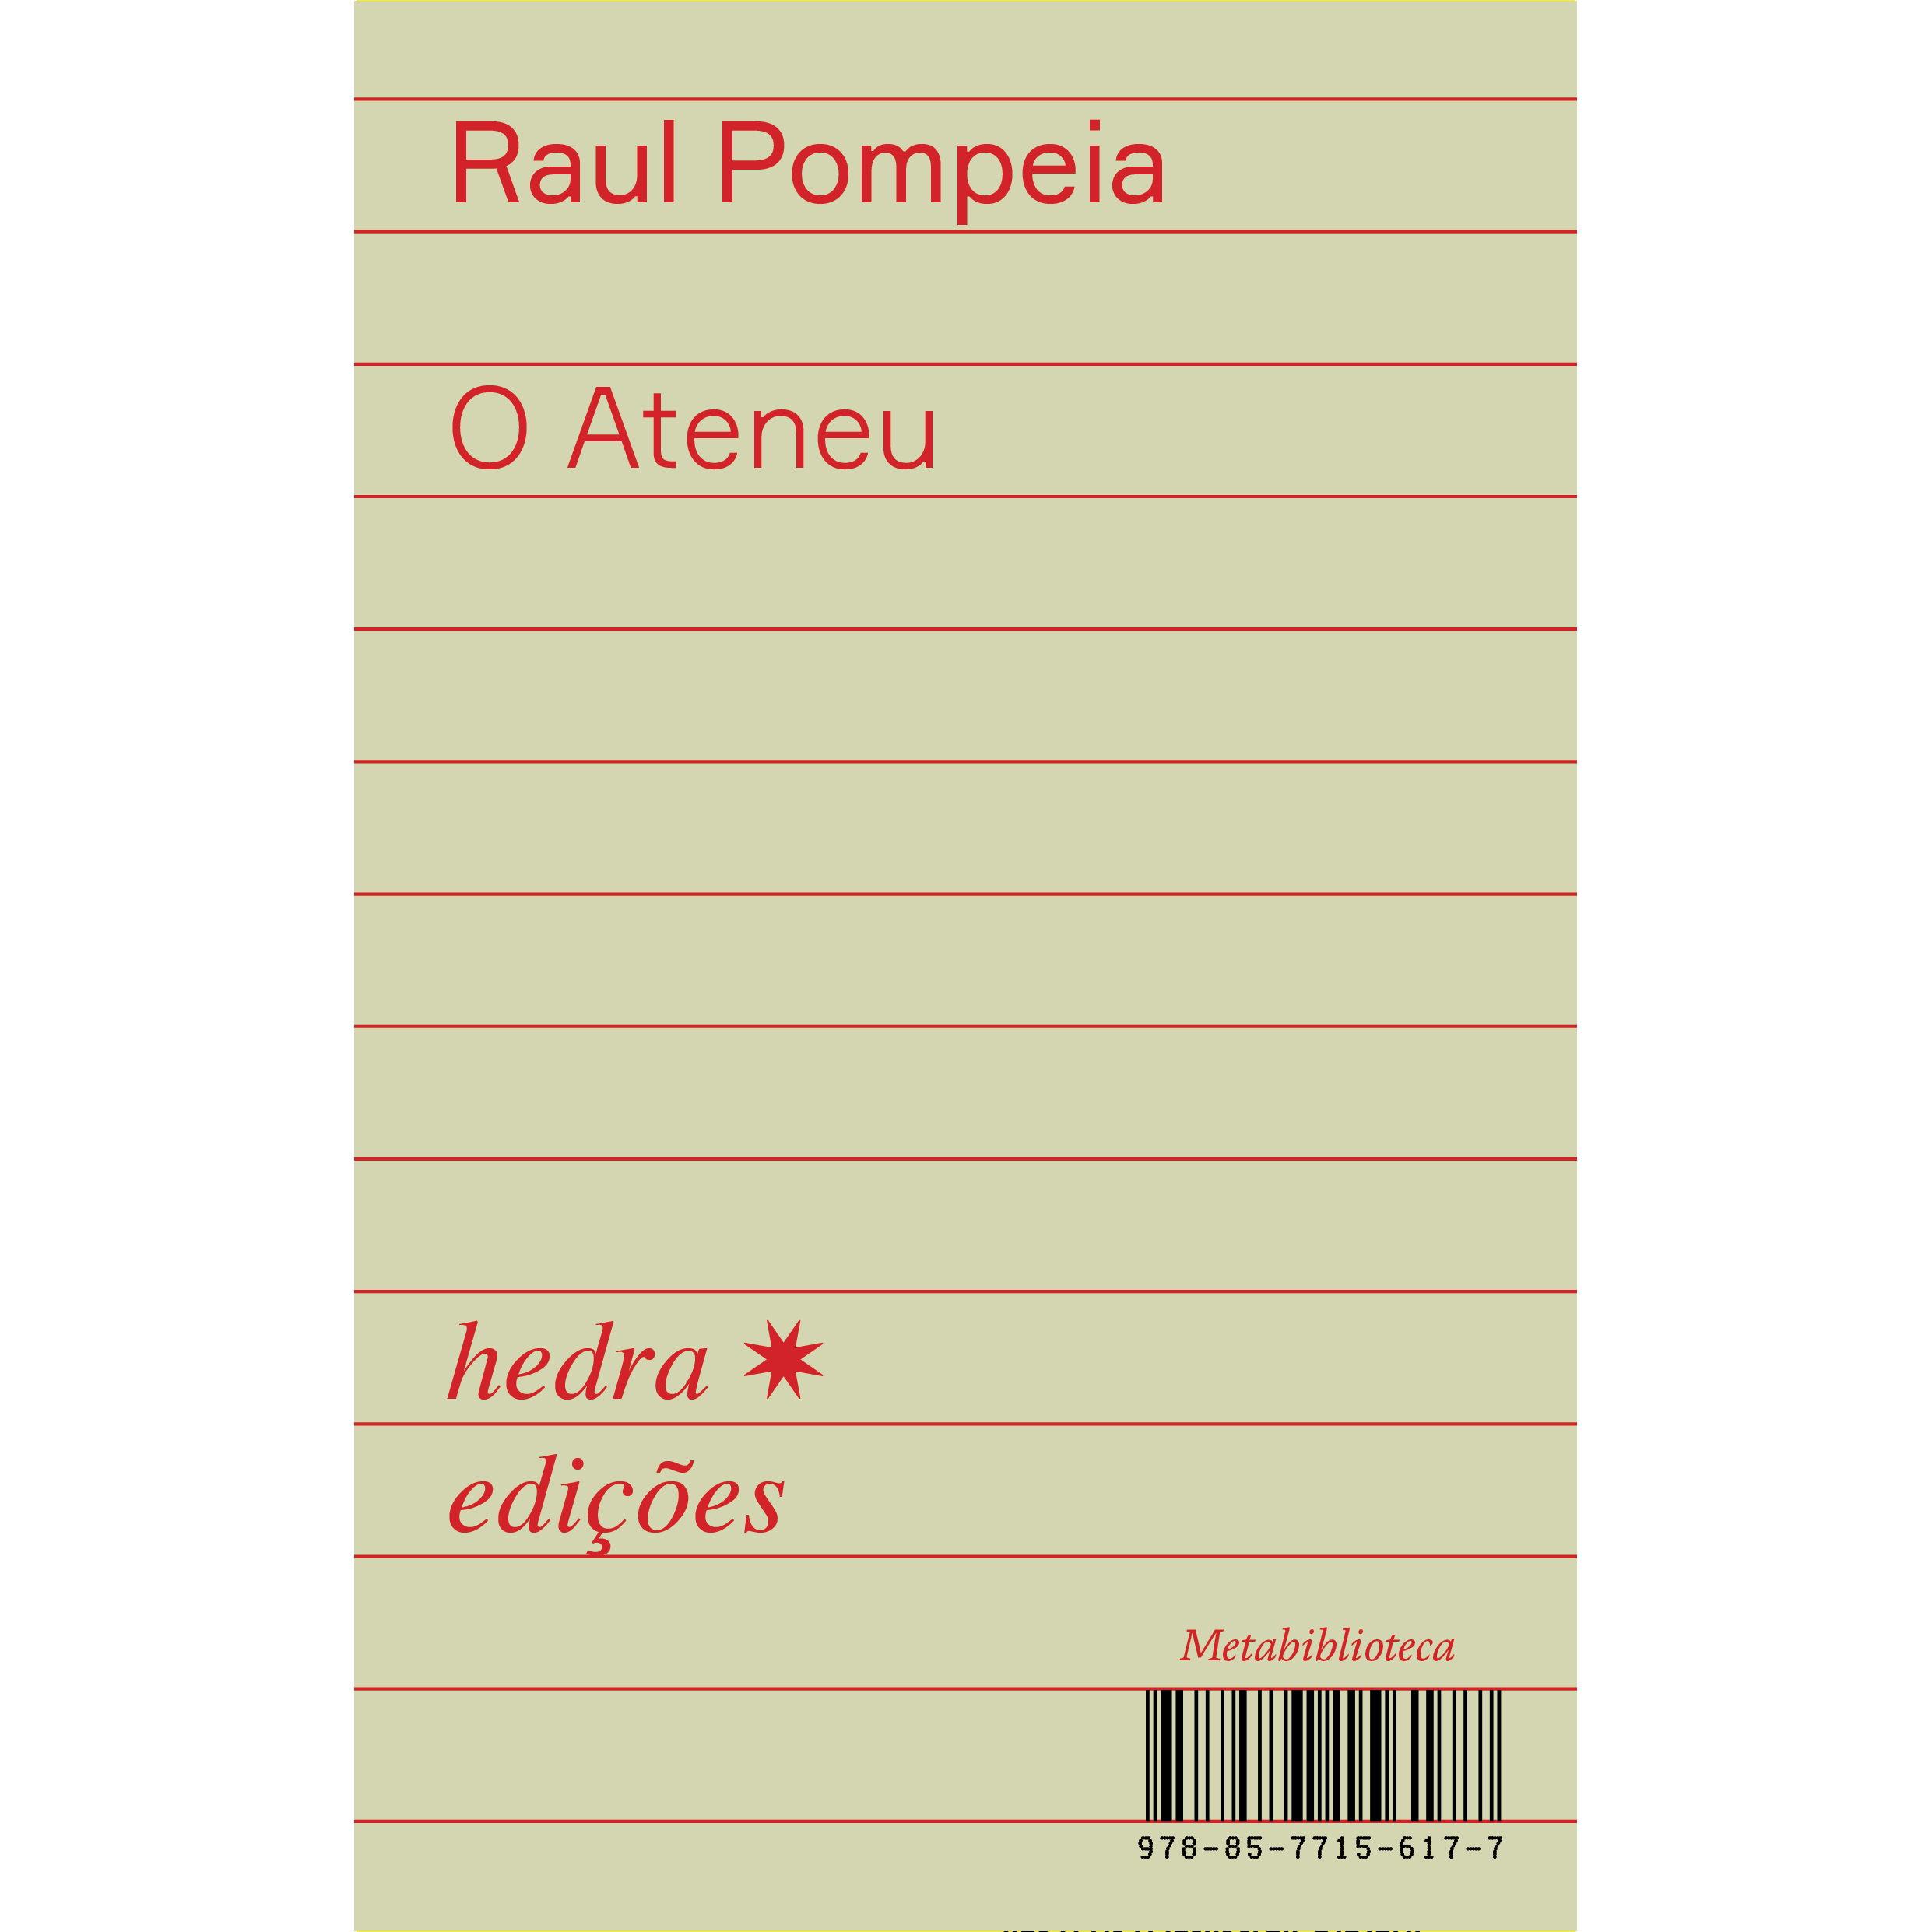
\includegraphics[width=92mm]{./grid/ateneu.jpg}
\end{center}

\hspace*{-7cm}\hrulefill\hspace*{-7cm}

\medskip

\noindent{}{\slsc{O ateneu}} foi publicado em capítulos,
no jornal carioca {\slsc{A gazeta de
notícias}}, entre 8 de abril e 18 de maio de 1888, e,
devido ao reconhecimento imediato, foi editado em livro no mesmo ano.
Escrito em apenas três meses, é considerado o maior romance brasileiro do
século \scalebox{.8}{XIX} depois dos romances realistas de Machado de Assis. Seu
enredo consiste na recordação do período de dois anos em que o narrador,
Sérgio, passa num tradicional colégio interno do Rio de Janeiro. O
ingresso no Ateneu marca as descobertas amargas que acompanharão o
narrador daí em diante, os sentimentos de desilusão, opressão e
desconfiança, componentes da profunda solidão humana. Seu sentido é o
de um ritual de passagem, em que o convívio com os colegas, os
professores e o diretor definem a afirmação moral, sexual e intelectual
de um menino de 11 anos. Difíceis de definir, o estilo e o
significado do romance geraram uma das mais profícuas polêmicas da
história da nossa literatura, aqui apresentada e antologizada
cronologicamente no final do volume.


\vfill
\enlargethispage{\baselineskip}


\hspace*{-.4cm}\begin{minipage}[c]{.5\linewidth}
\small{
{\Formular{\textbf{
\hspace*{-.1cm}Título: O ateneu\\
Autor: Raul Pompéia\\ 
ISBN: 978-85-7715-638-2\\
Páginas: ???\\
Formato: 13,3x21cm\\
Preço: R\$ ????\\
Editora: Hedra\\
Disponibilidade: 31/07/2020
}}}}
\end{minipage}

\pagebreak

\hspace{.5cm}

\begin{center}
\hspace*{-2.5cm}\raisebox{6.8cm}{\rotatebox[origin=t]{90}{\huge\Formular{\textbf{Lançamento}}}}
\hspace*{2.5cm}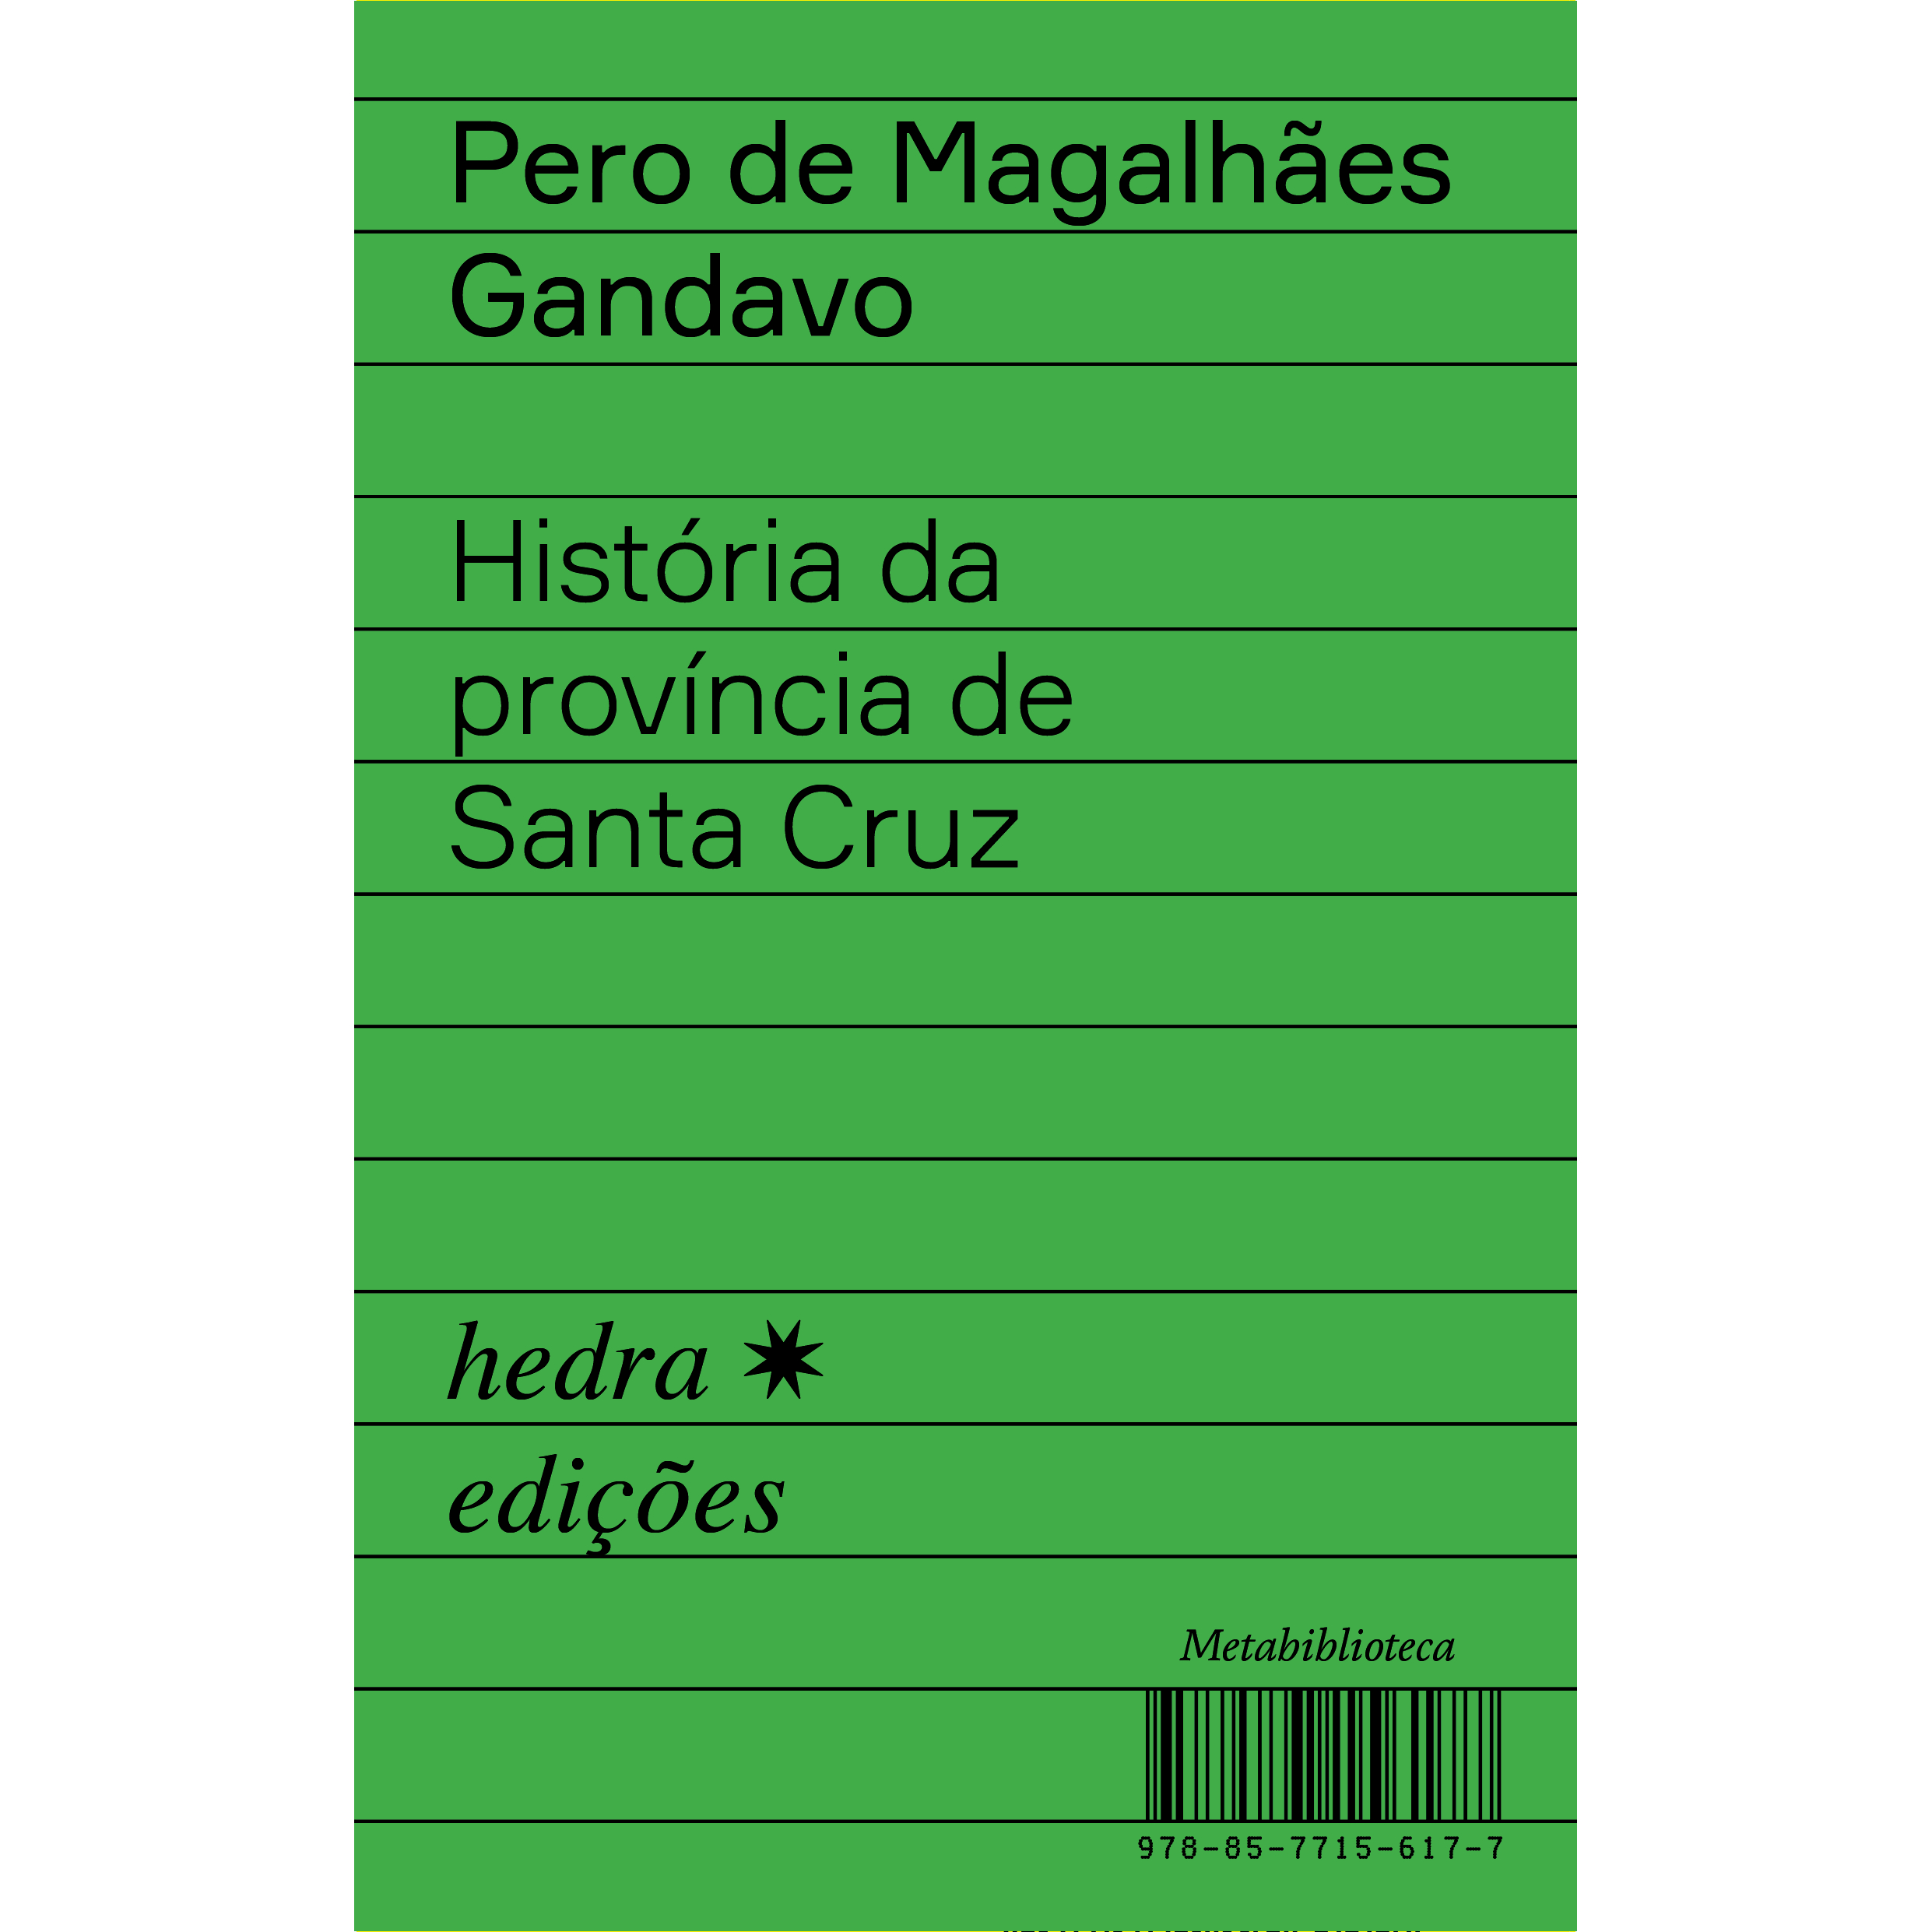
\includegraphics[width=92mm]{./grid/gandavo.jpg}
\end{center}

\hspace*{-7cm}\hrulefill\hspace*{-7cm}

\medskip

\noindent{}{\slsc{História da província de Santa Cruz}}, de 1576, foi lido como “relato de viajante” ou como “nossa primeira história”, entendido como testemunho de impressões antigas dos portugueses nas terras d’além"-mar. Contudo, esta simples história ou tratado descritivo da “costa do Brasil” teve circulação muito restrita à época, o que leva a crer que foi recolhida e destruída após sua impressão. Permaneceu praticamente ignorada até 1837, quando foi reconsiderada em edição e tradução francesa.

A obscuridade do livro nos séculos seguintes à sua publicação é tanto mais estranha tendo"-se em vista que, por intermédio de uma elegia e um soneto de Camões, o livro é dedicado a um varão de armas em carreira promissora nas Índias portuguesas, tendo sido impresso pela mesma oficina tipográfica que compôs {\slsc{Os Lusíadas}} (1572). Diferente de um testemunho empírico, o livro é composto conforme a ideia de gênero histórico, retoricamente regrado, em que o historiador, apoiado pelo aconselhamento ético da Igreja Católica, tem por fim exaltar, pelo discurso, ações virtuosas de pessoas de caráter elevado e eventos providenciais.

\vfill

\hspace*{-.4cm}\begin{minipage}[c]{.5\linewidth}
\small{
{\Formular{\textbf{
\hspace*{-.1cm}Título: História da província de Santa Cruz\\
Autor: Gandavo\\ 
ISBN: 978-85-7715-639-9\\
Páginas: ???\\
Formato: 13,3x21cm\\
Preço: R\$ ????\\
Editora: Hedra\\
Disponibilidade: 31/07/2020
}}}}
\end{minipage}

\pagebreak

\hspace{.5cm}

\begin{center}
\hspace*{.5cm}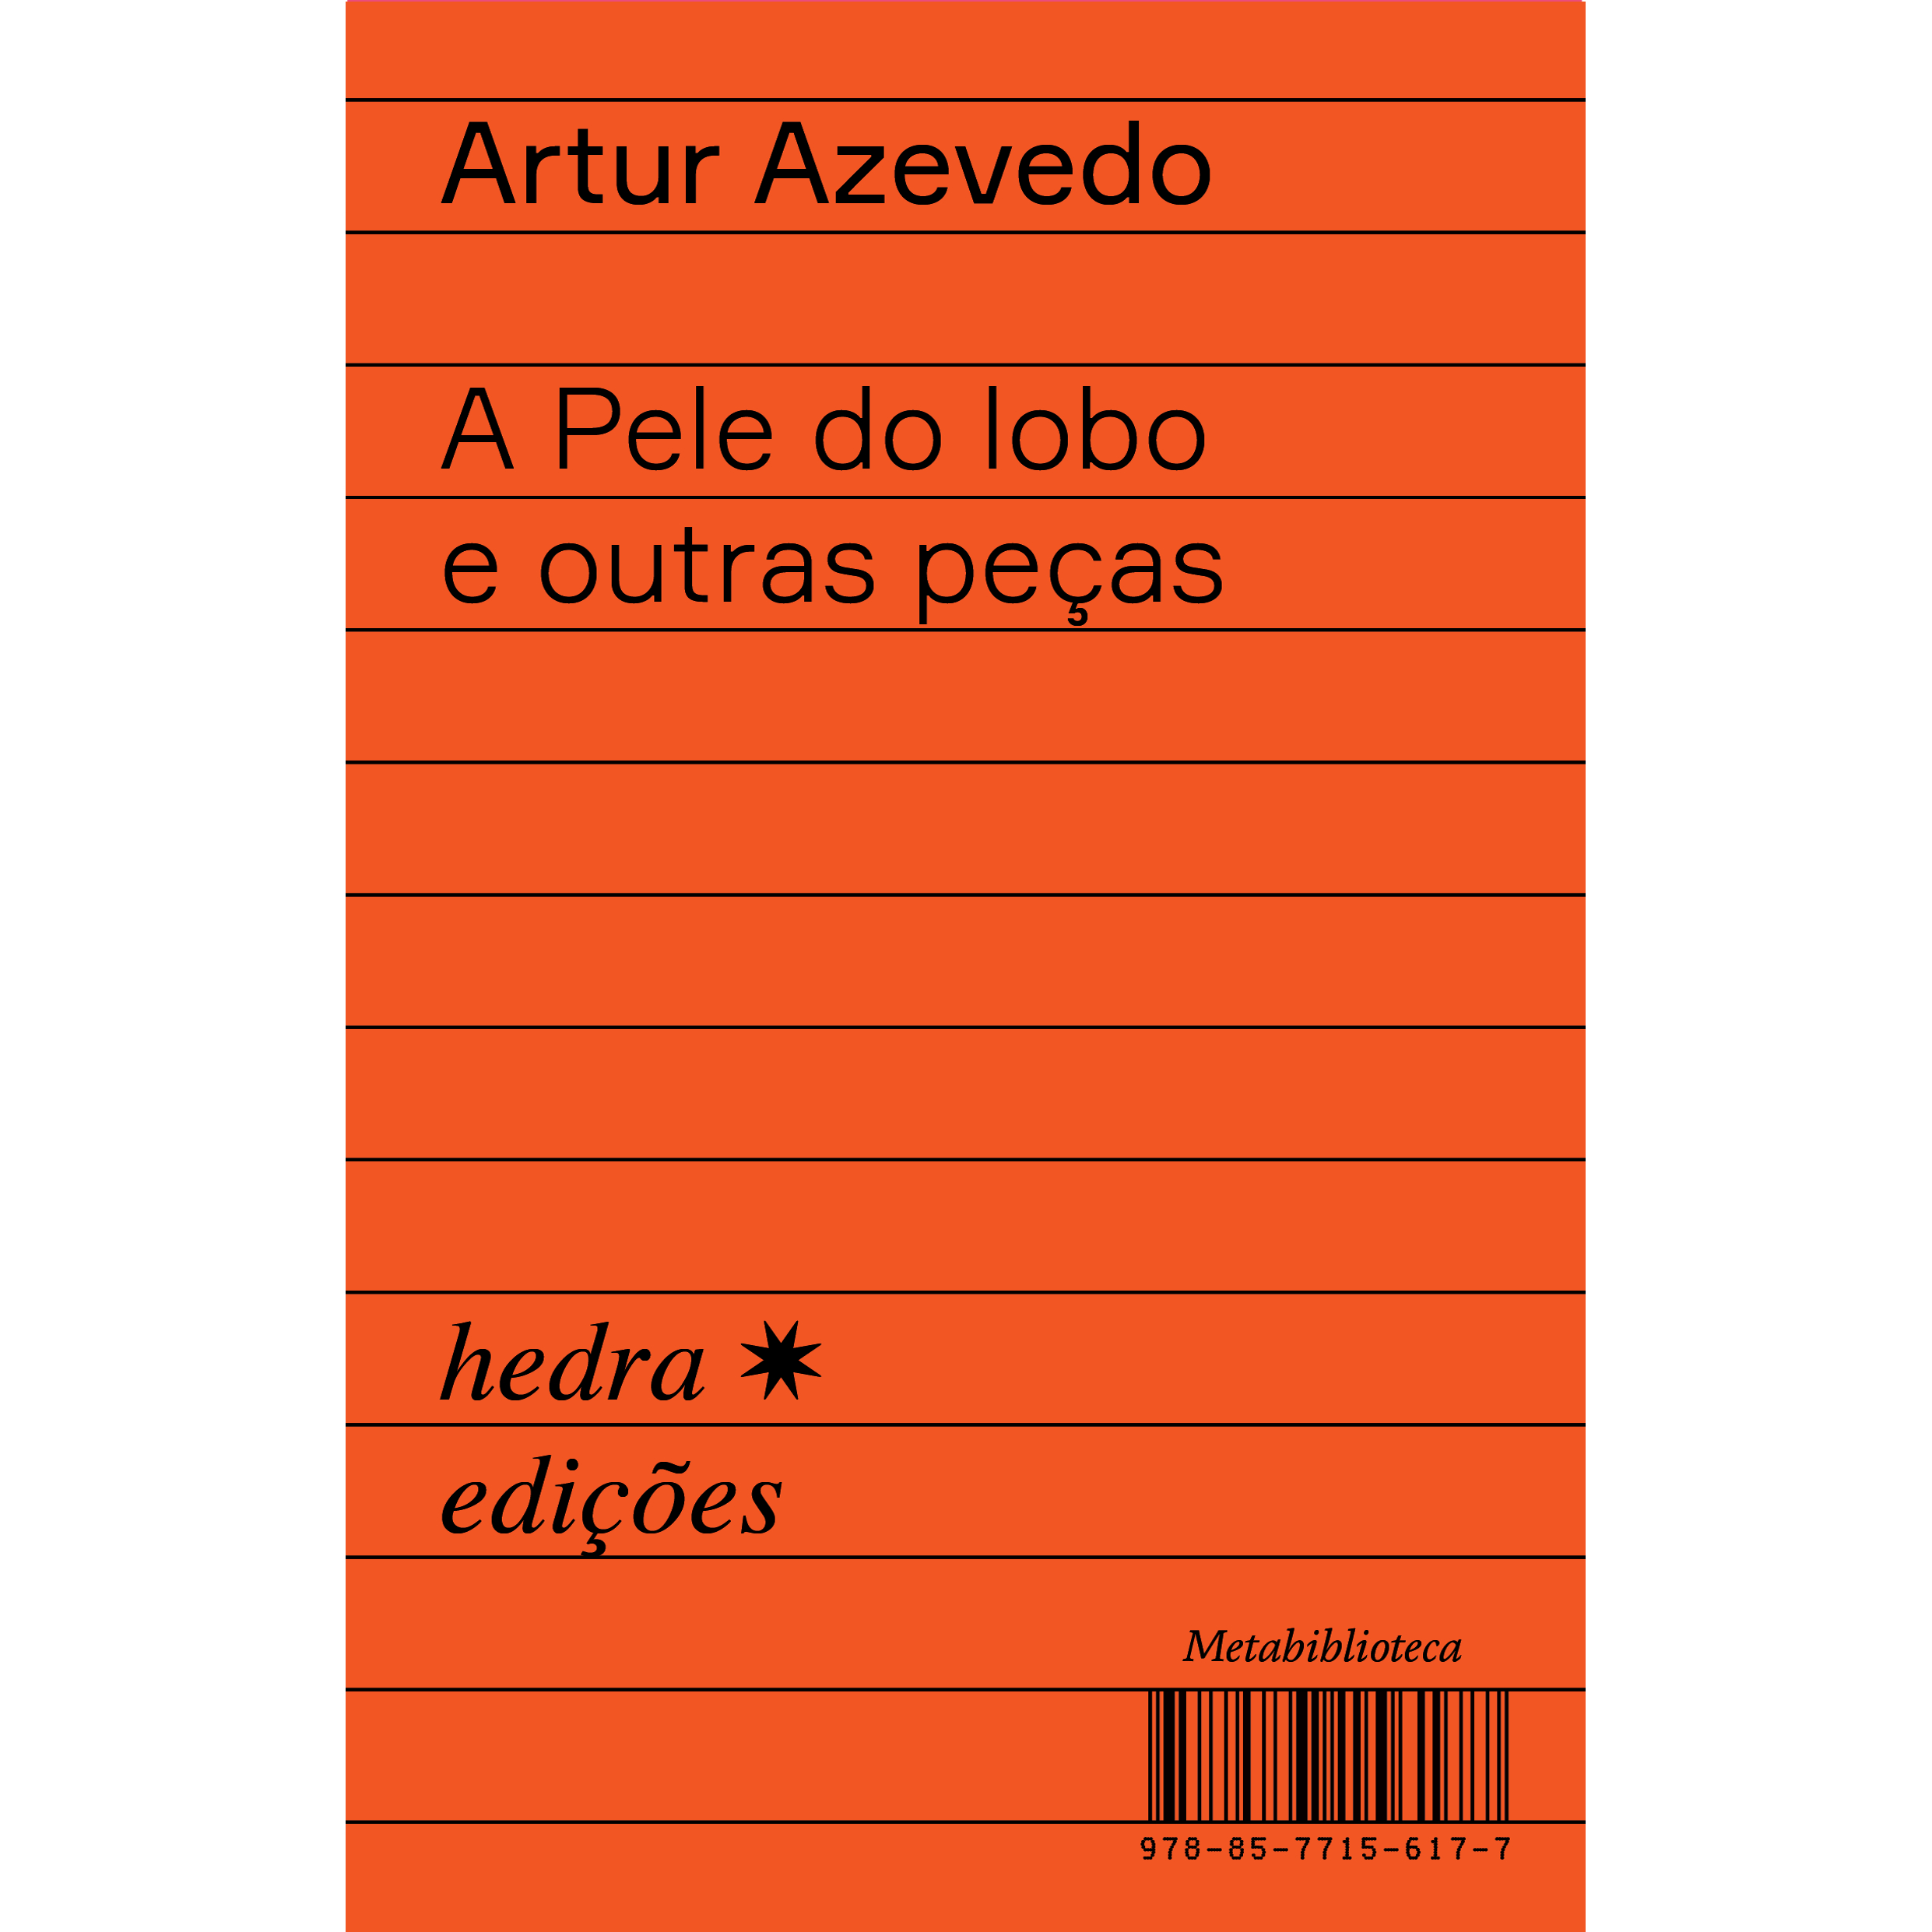
\includegraphics[width=92mm]{./grid/azevedo.jpg}
\end{center}

\hspace*{-7cm}\hrulefill\hspace*{-7cm}

\medskip

\noindent{}{\slsc{A pele do lobo e outras peças}} inclui cinco textos curtos de Artur de Azevedo, cuja temática gira em torno de costumes nacionais. {\slsc{Amor por anexins}} (1870) foi a primeira peça do autor. {\slsc{A pele do lobo}} (1875) faz uma sátira divertida ao sistema de policiamento do Império. {\slsc{O Oráculo}} (1907) é um texto que dialoga com a tradição da comédia. {\slsc{Como eu me diverti!}} (1893) e {\slsc{O Cordão}} (1908) tratam do carnaval e são exemplos importantes da conturbada posição de Artur de Azevedo entre os escritores de seu tempo, por ser um autor eminentemente popular. Azevedo é um dos melhores comediógrafos brasileiros e foi nosso primeiro grande homem de teatro. Além de dramaturgo foi cronista, contista e poeta. Escreveu mais de duzentas peças, entre originais, traduções e adaptações.


\vfill

\hspace*{-.4cm}\begin{minipage}[c]{.5\linewidth}
\small{
{\Formular{\textbf{
\hspace*{-.1cm}Título: A pele do lobo e outras peças\\
Autor: Artur de Azevedo\\ 
ISBN: 978-85-7715-641-2\\
Páginas: ???\\
Formato: 13,3x21cm\\
Preço: R\$ ????\\
Editora: Hedra\\
Disponibilidade: 31/07/2020
}}}}
\end{minipage}

\pagebreak

\hspace{.5cm}

\begin{center}
\hspace*{-2.5cm}\raisebox{6.8cm}{\rotatebox[origin=t]{90}{\huge\Formular{\textbf{Lançamento}}}}
\hspace*{2.5cm}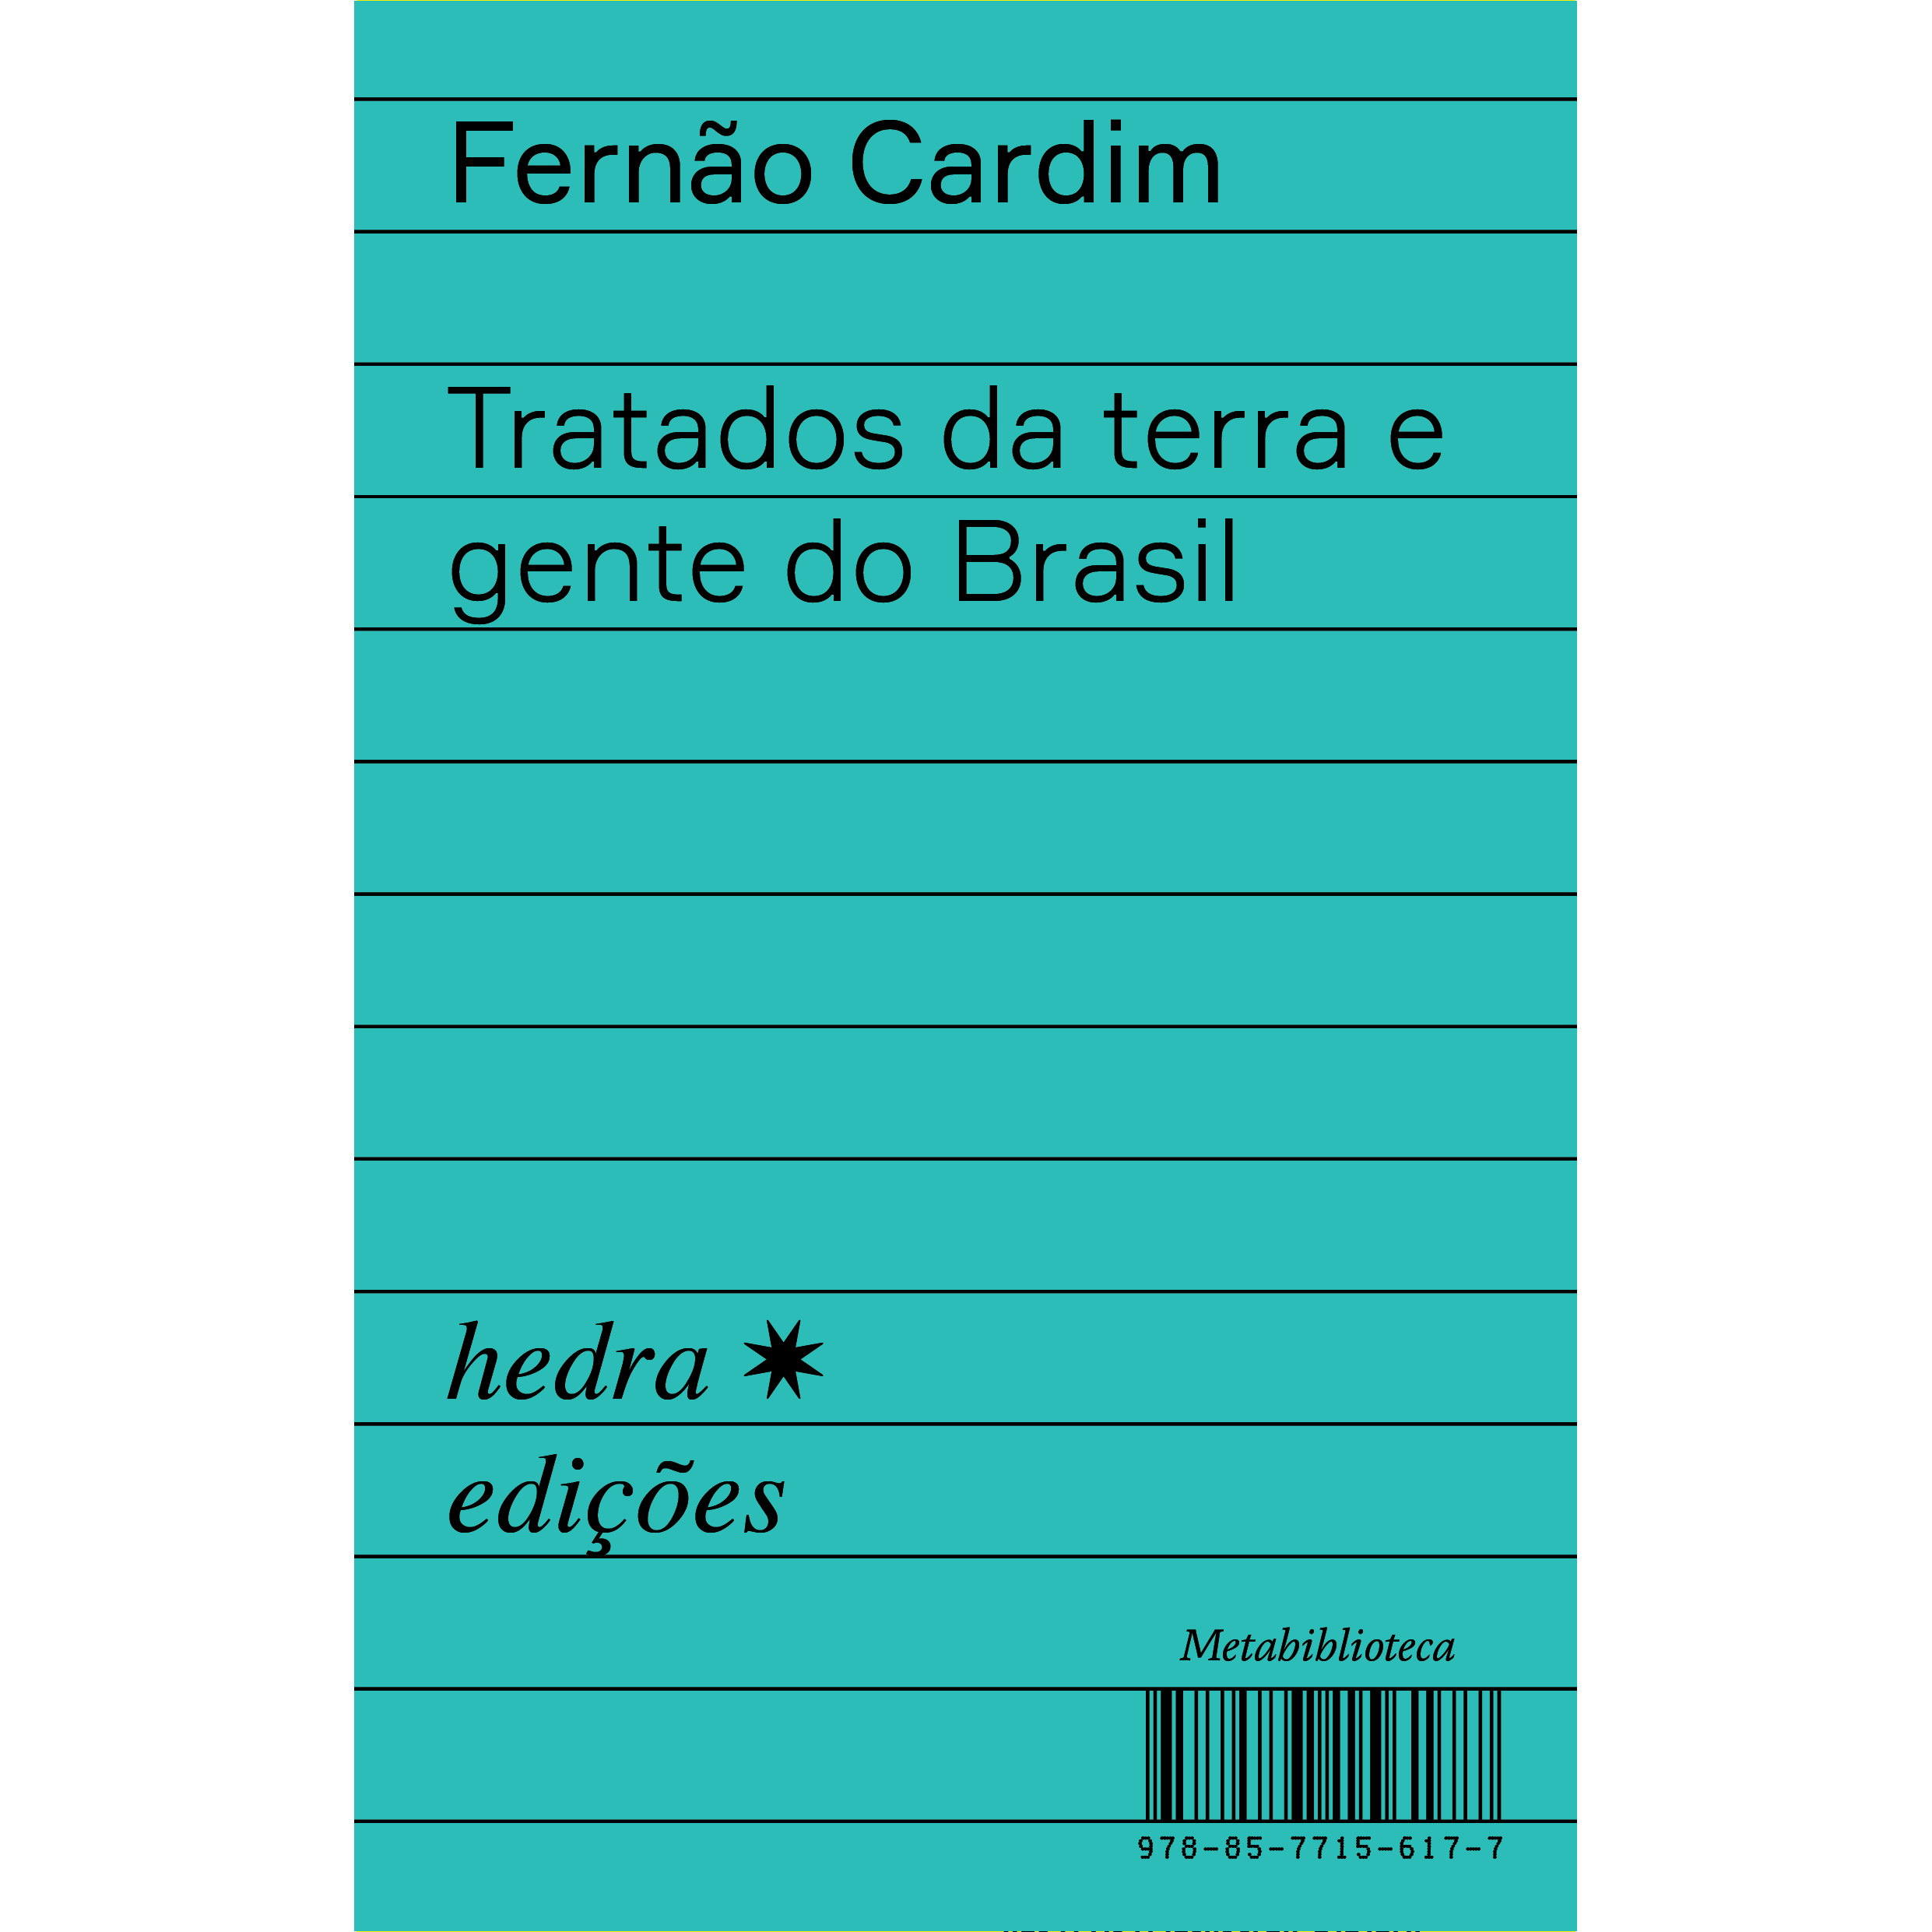
\includegraphics[width=92mm]{./grid/cardim.jpg}
\end{center}

\hspace*{-7cm}\hrulefill\hspace*{-7cm}

\medskip

\noindent{}{\slsc{Tratados da terra e gente do Brasil}} foram escritos entre 1583 e 1601 pelo padre jesuíta Fernão Cardim, nos anos seguintes à sua chegada ao Brasil, quando desempenhou o cargo de secretário do Padre Visitador Cristóvão de Gouveia. O livro manteve"-se inédito em língua portuguesa até 1847, embora tenha sido publicado parcialmente em inglês, em 1625, com atribuição a outro autor.

Os tratados de Cardim permitem"-nos ter um conhecimento da terra brasileira do Quinhentos e dos povos ameríndios, assim como do papel dos jesuítas nessa região e dos hábitos da vida nos engenhos. A obra é de interesse não apenas pela descrição da terra e do clima, já que aborda ainda a fauna e a flora, e os seus habitantes, procurando salientar a importância que esta terra poderia vir a ter no futuro, pois já se evidenciava como sendo “outro Portugal”. 

\vfill

\hspace*{-.4cm}\begin{minipage}[c]{.5\linewidth}
\small{
{\Formular{\textbf{
\hspace*{-.1cm}Título: Tratados da terra e gente do Brasil\\
Autor: Fernão Cardim\\ 
ISBN: 978-85-7715-642-9\\
Páginas: ???\\
Formato: 13,3x21cm\\
Preço: R\$ ????\\
Editora: Hedra\\
Disponibilidade: 31/07/2020
}}}}
\end{minipage}

\pagebreak

\hspace{.5cm}

\begin{center}
\hspace*{.5cm}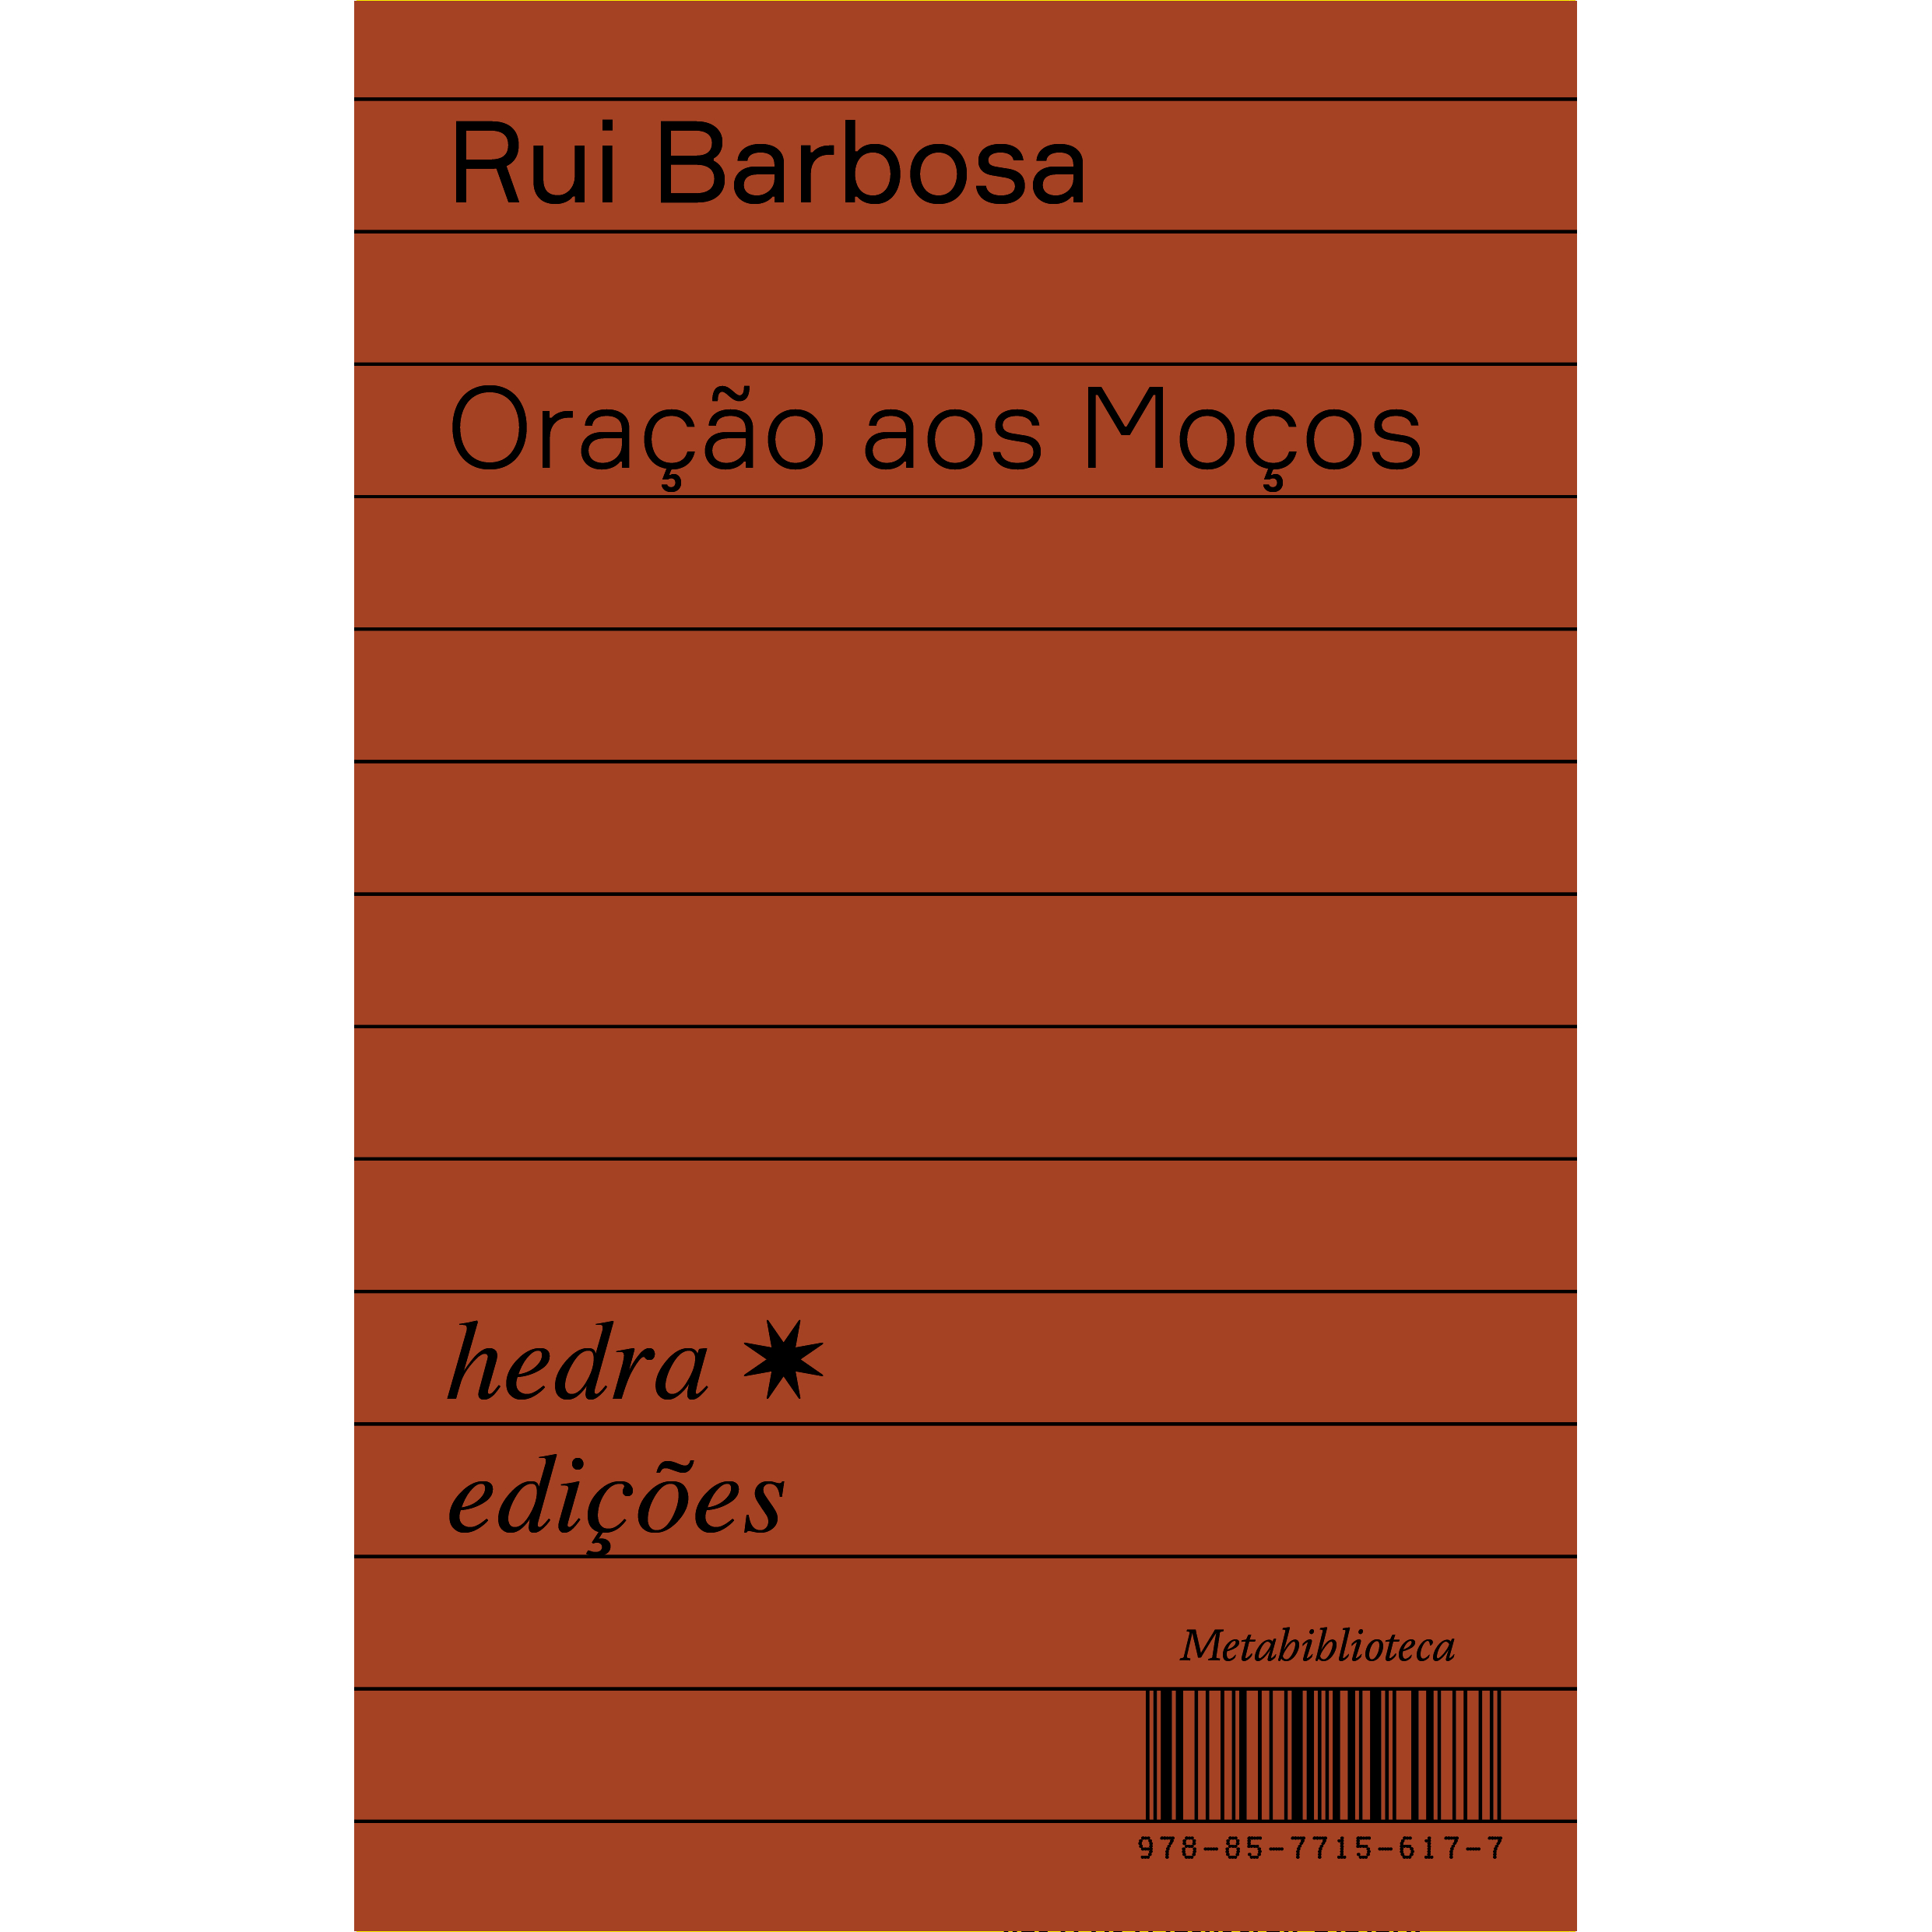
\includegraphics[width=92mm]{./grid/barbosa.jpg}
\end{center}

\hspace*{-7cm}\hrulefill\hspace*{-7cm}

\medskip

\noindent{}{\slsc{Oração aos moços}} é um dos mais célebres discursos de Rui
Barbosa, escrito para paraninfar os formandos da
turma de 1920 da Faculdade de Direito do Largo de São Francisco, em São
Paulo. Impedido de comparecer,  por problemas de saúde, o texto foi
lido pelo professor Reinaldo Porchat. Trata"-se de uma das mais
brilhantes reflexões produzidas pelo jurista sobre o papel do
magistrado e a missão do advogado.

O autor faz um balanço de sua vida
como advogado, jornalista e político, como exemplo para as novas
gerações. Esta edição traz ainda, em apêndice, a famosa carta
a Evaristo de Morais que ficaria conhecida como ``O dever do advogado'',
na qual Rui trata com a propriedade e a elegância que lhe são peculiares
dos dilemas de ética profissional com os quais se deparam os que 
seguem a carreira jurídica. 

\vfill

\hspace*{-.4cm}\begin{minipage}[c]{.5\linewidth}
\small{
{\Formular{\textbf{
\hspace*{-.1cm}Título: Oração aos moços\\
Autor: Rui Barbosa\\ 
ISBN: 978-85-7715-643-6\\
Páginas: ???\\
Formato: 13,3x21cm\\
Preço: R\$ ????\\
Editora: Hedra\\
Disponibilidade: 31/07/2020
}}}}
\end{minipage}

\pagebreak

\hspace{.5cm}

\begin{center}
\hspace*{-2.5cm}\raisebox{6.8cm}{\rotatebox[origin=t]{90}{\huge\Formular{\textbf{Lançamento}}}}
\hspace*{2.5cm}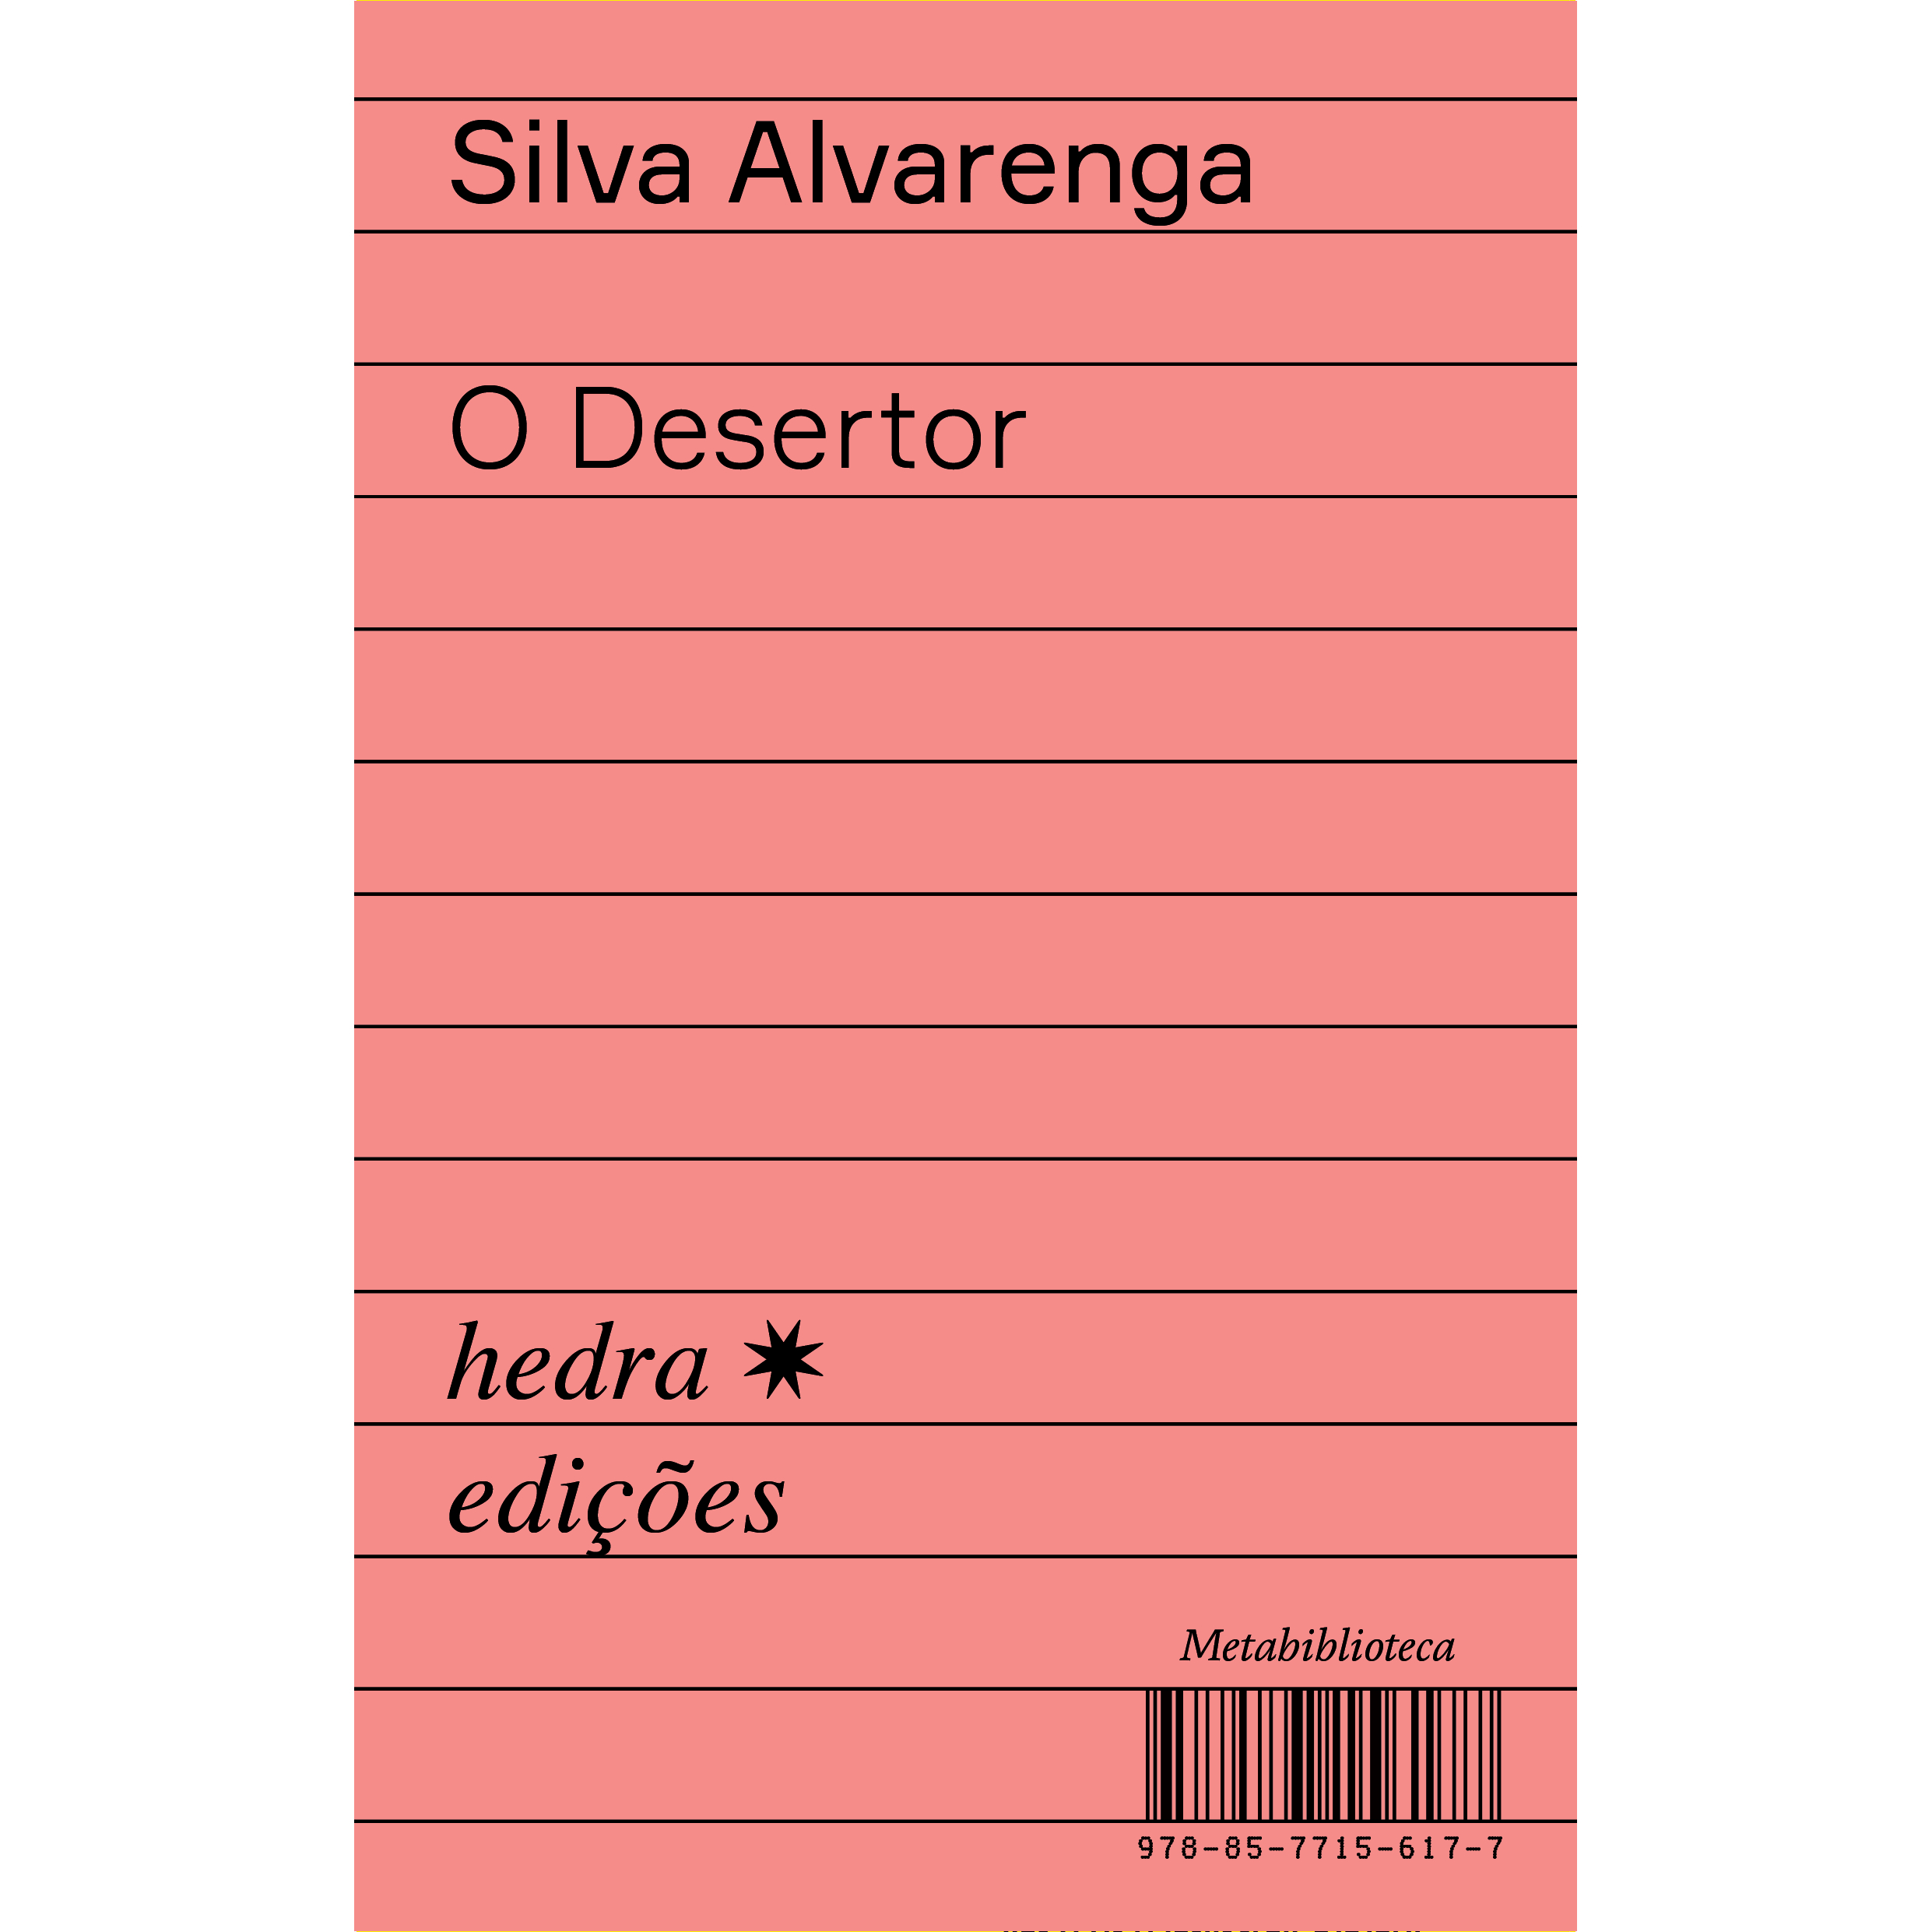
\includegraphics[width=92mm]{./grid/desertor.jpg}
\end{center}

\hspace*{-7cm}\hrulefill\hspace*{-7cm}

\medskip

\noindent{}A fábula cômica é constituída pelas peripécias de um grupo de estudantes guiados pelo professor Tibúrcio, personificação da Ignorância, expulsa de Coimbra pelo Marquês de Pombal, que restituíra a Verdade ao trono na velha instituição de ensino. Aristotelicamente fundada, a fábula é cômica, por definição, porque imita homens e ações piores, descreve matérias baixas e dignas de opróbrio. Assim, acumula tipos socialmente inferiores ou moralmente deformados, relata brigas comezinhas, com unhas e dentes, tumultos e bebedeiras, em lugar de triunfos da virtude.

Quando {\slsc{O desertor: poema herói-cômico}} é lançado em 1774, Silva Alvarenga tinha 24 anos e era aluno da Universidade de Coimbra, recentemente reformada. Com efeito, o argumento heroico do poema é a Reforma dos Estatutos da Universidade de Coimbra, o que lhe dá sentido didático e elogioso. Por outro lado, a dissociação deliberada entre o assunto baixo e a elocução ornada com palavras graves dignas de grandes feitos é o que fundamenta o subtítulo do poema e o enquadra num gênero misto.

\vfill

\hspace*{-.4cm}\begin{minipage}[c]{.5\linewidth}
\small{
{\Formular{\textbf{
\hspace*{-.1cm}Título: O desertor — poema herói"-cômico\\
Autor: Silva Alvarenga\\ 
ISBN: 978-85-7715-644-3\\
Páginas: ???\\
Formato: 13,3x21cm\\
Preço: R\$ ????\\
Editora: Hedra\\
Disponibilidade: 31/07/2020
}}}}
\end{minipage}

\pagebreak

\hspace{.5cm}

\begin{center}
\hspace*{.5cm}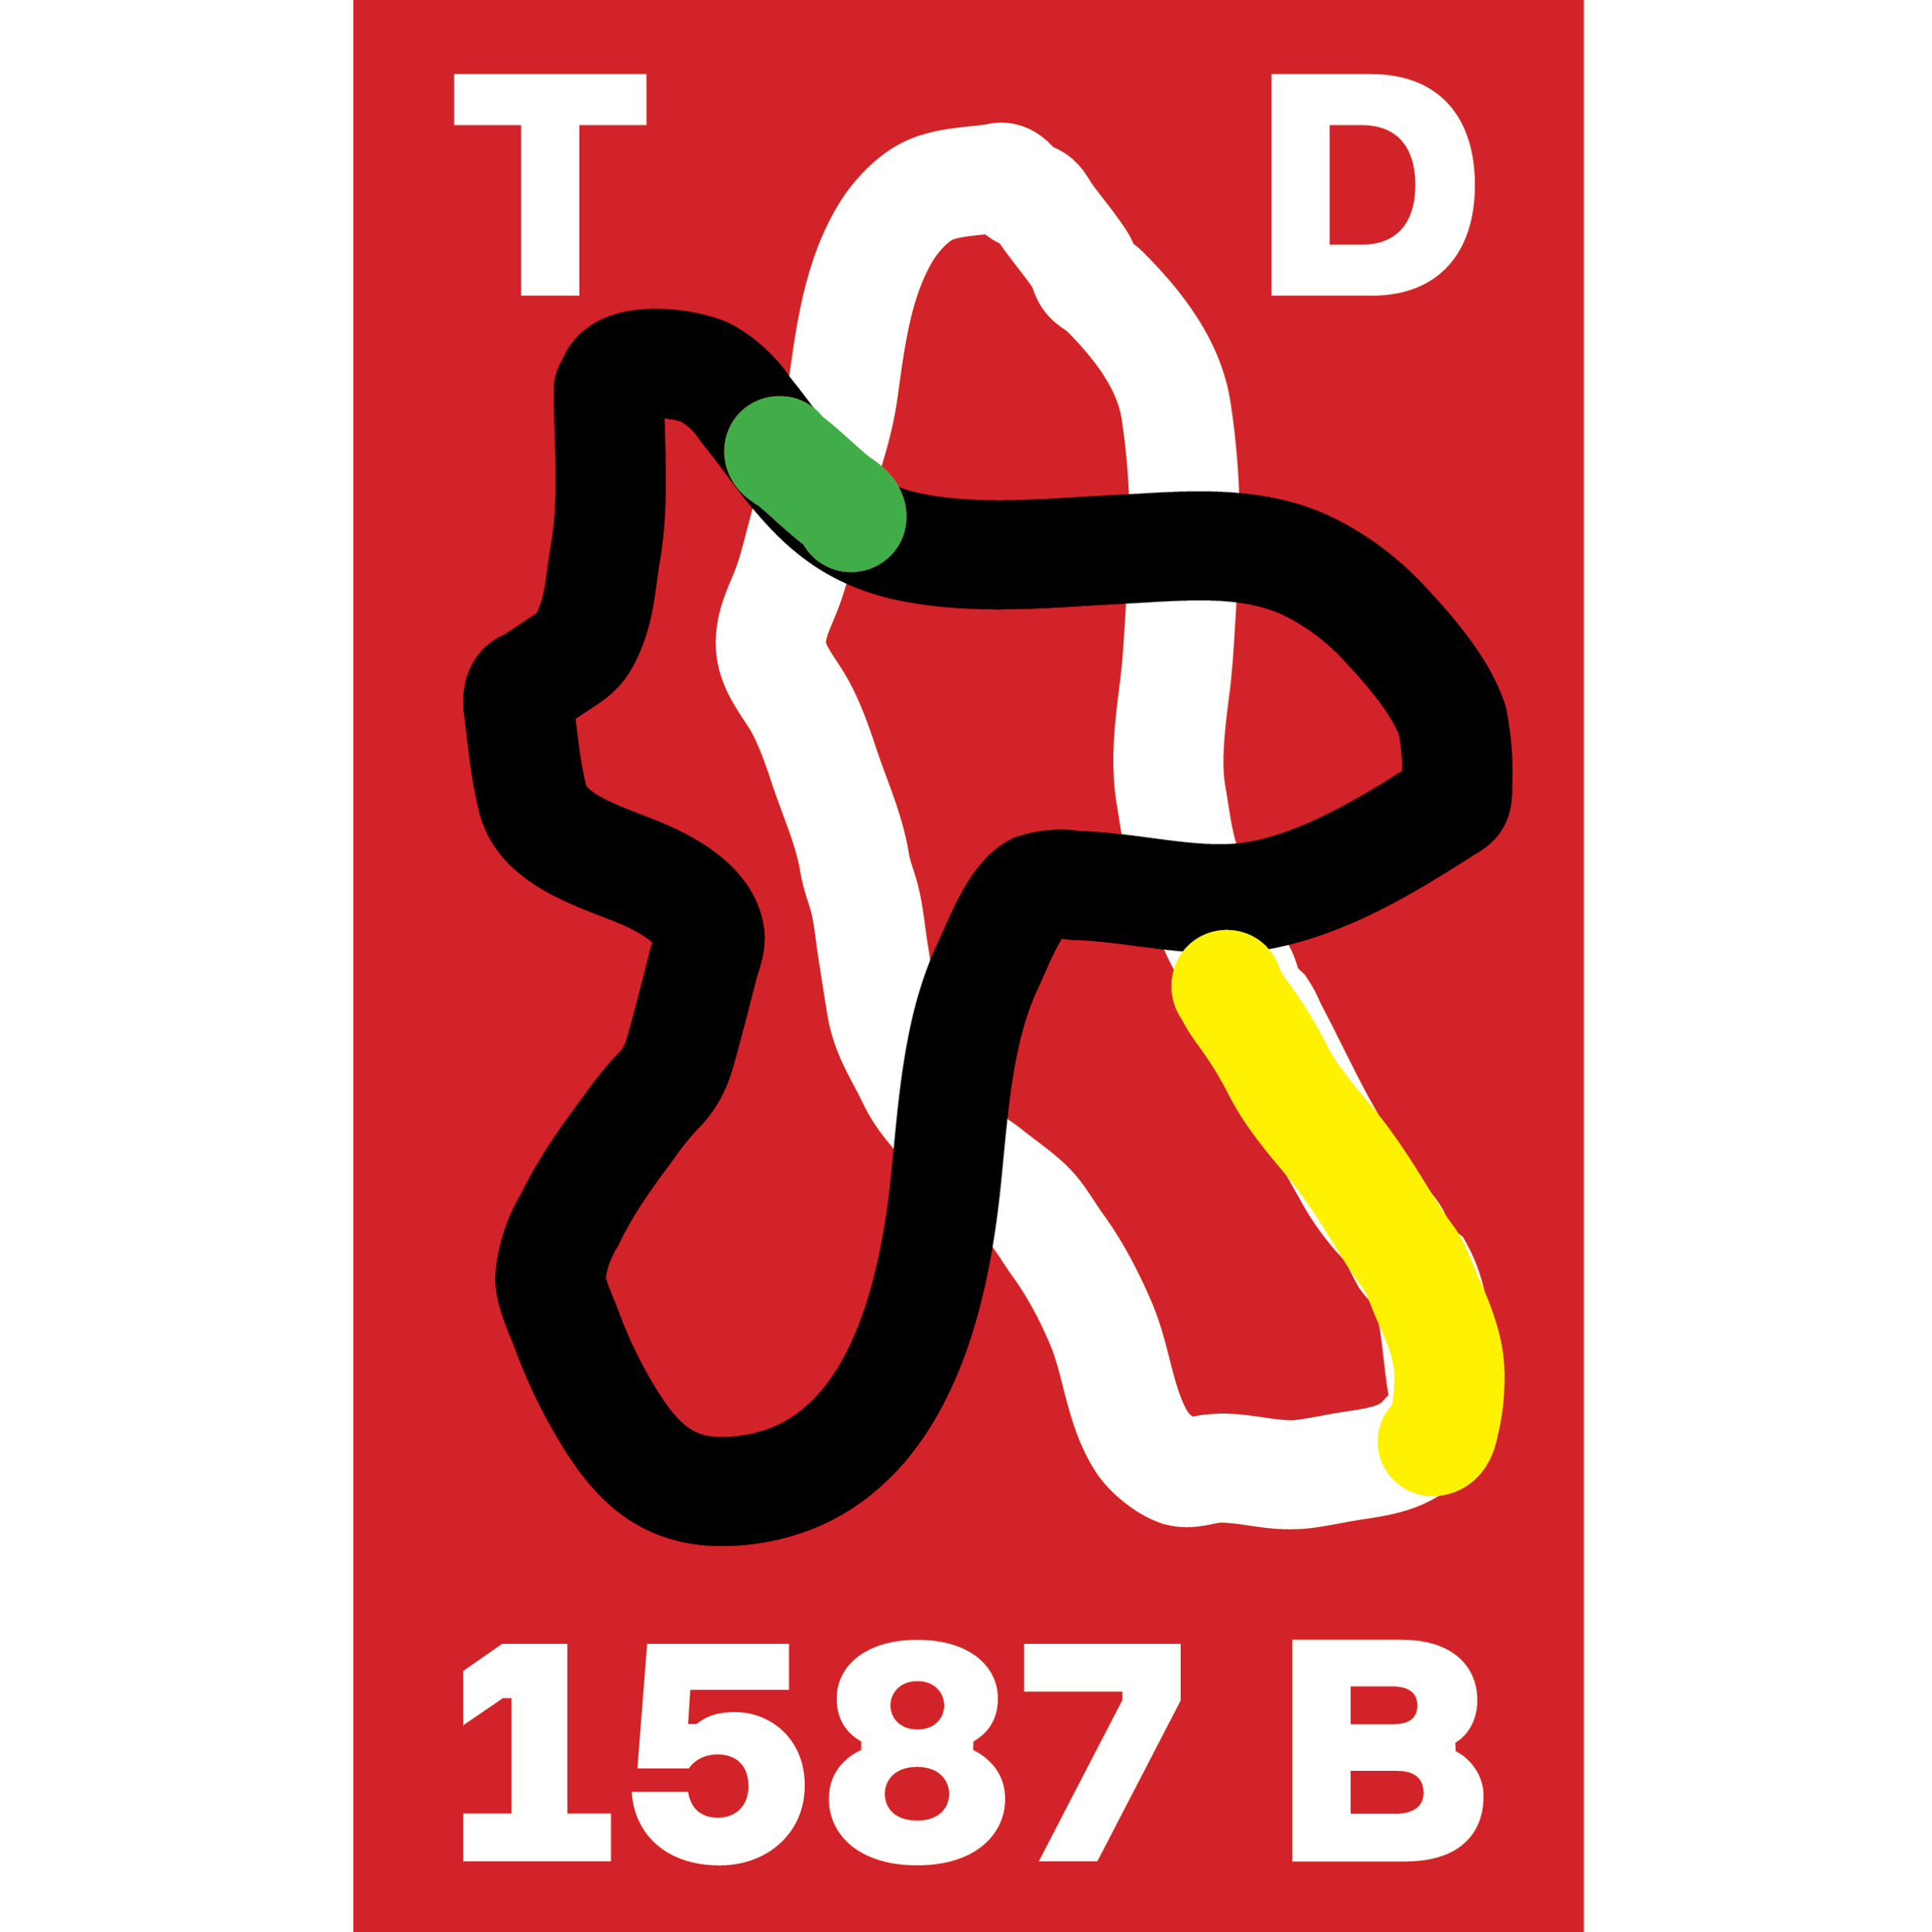
\includegraphics[width=92mm]{./grid/tratado.jpg}
\end{center}

\hspace*{-7cm}\hrulefill\hspace*{-7cm}

\medskip

\noindent{}{\slsc{Tratado descritivo do Brasil em 1587}} reúne dois textos de
Gabriel Soares de Sousa enviados a um influente conselheiro do rei
Filipe \scalebox{.8}{II} de Espanha, no intuito de oferecer à Coroa informações acerca
da situação da colônia portuguesa e demonstrar o conhecimento do autor
sobre aquelas terras.  O {\slsc{Roteiro geral com largas informações
de toda a costa do Brasil}} e o {\slsc{Memorial e declaração das
grandezas da Bahia de Todos os Santos, de sua fertilidade e das
notáveis partes que tem}}, que permaneceram
inéditos e anônimos ou apócrifos até o século \scalebox{.8}{XIX}, quando foram
recuperados, reunidos e publicados integralmente.

Desde então, a obra tem despertado grande interesse dos estudiosos do
início da colonização do Brasil e é considerada por muitos o mais
importante texto quinhentista sobre o assunto. É fonte indispensável a
diferentes áreas do conhecimento, como botânica, geografia, história e
antropologia, pois as minuciosas descrições apresentadas por Soares
fornecem preciosas informações a respeito da fauna, flora, acidentes
geográficos, povos nativos e engenhos da costa do Brasil no
século \scalebox{.8}{XVI}.

\vfill

\hspace*{-.4cm}\begin{minipage}[c]{.5\linewidth}
\small{
{\Formular{\textbf{
\hspace*{-.1cm}Título: Tratado descritivo do Brasil em 1587\\
Autor: Gabriel Soares de Sousa\\ 
ISBN: 978-85-7715-645-0\\
Páginas: ???\\
Formato: 13,3x21cm\\
Preço: R\$ ????\\
Editora: Hedra\\
Disponibilidade: 31/07/2020
}}}}
\end{minipage}

\pagebreak

\hspace{.5cm}

\begin{center}
\hspace*{-2.5cm}\raisebox{6.8cm}{\rotatebox[origin=t]{90}{\huge\Formular{\textbf{Lançamento}}}}
\hspace*{2.5cm}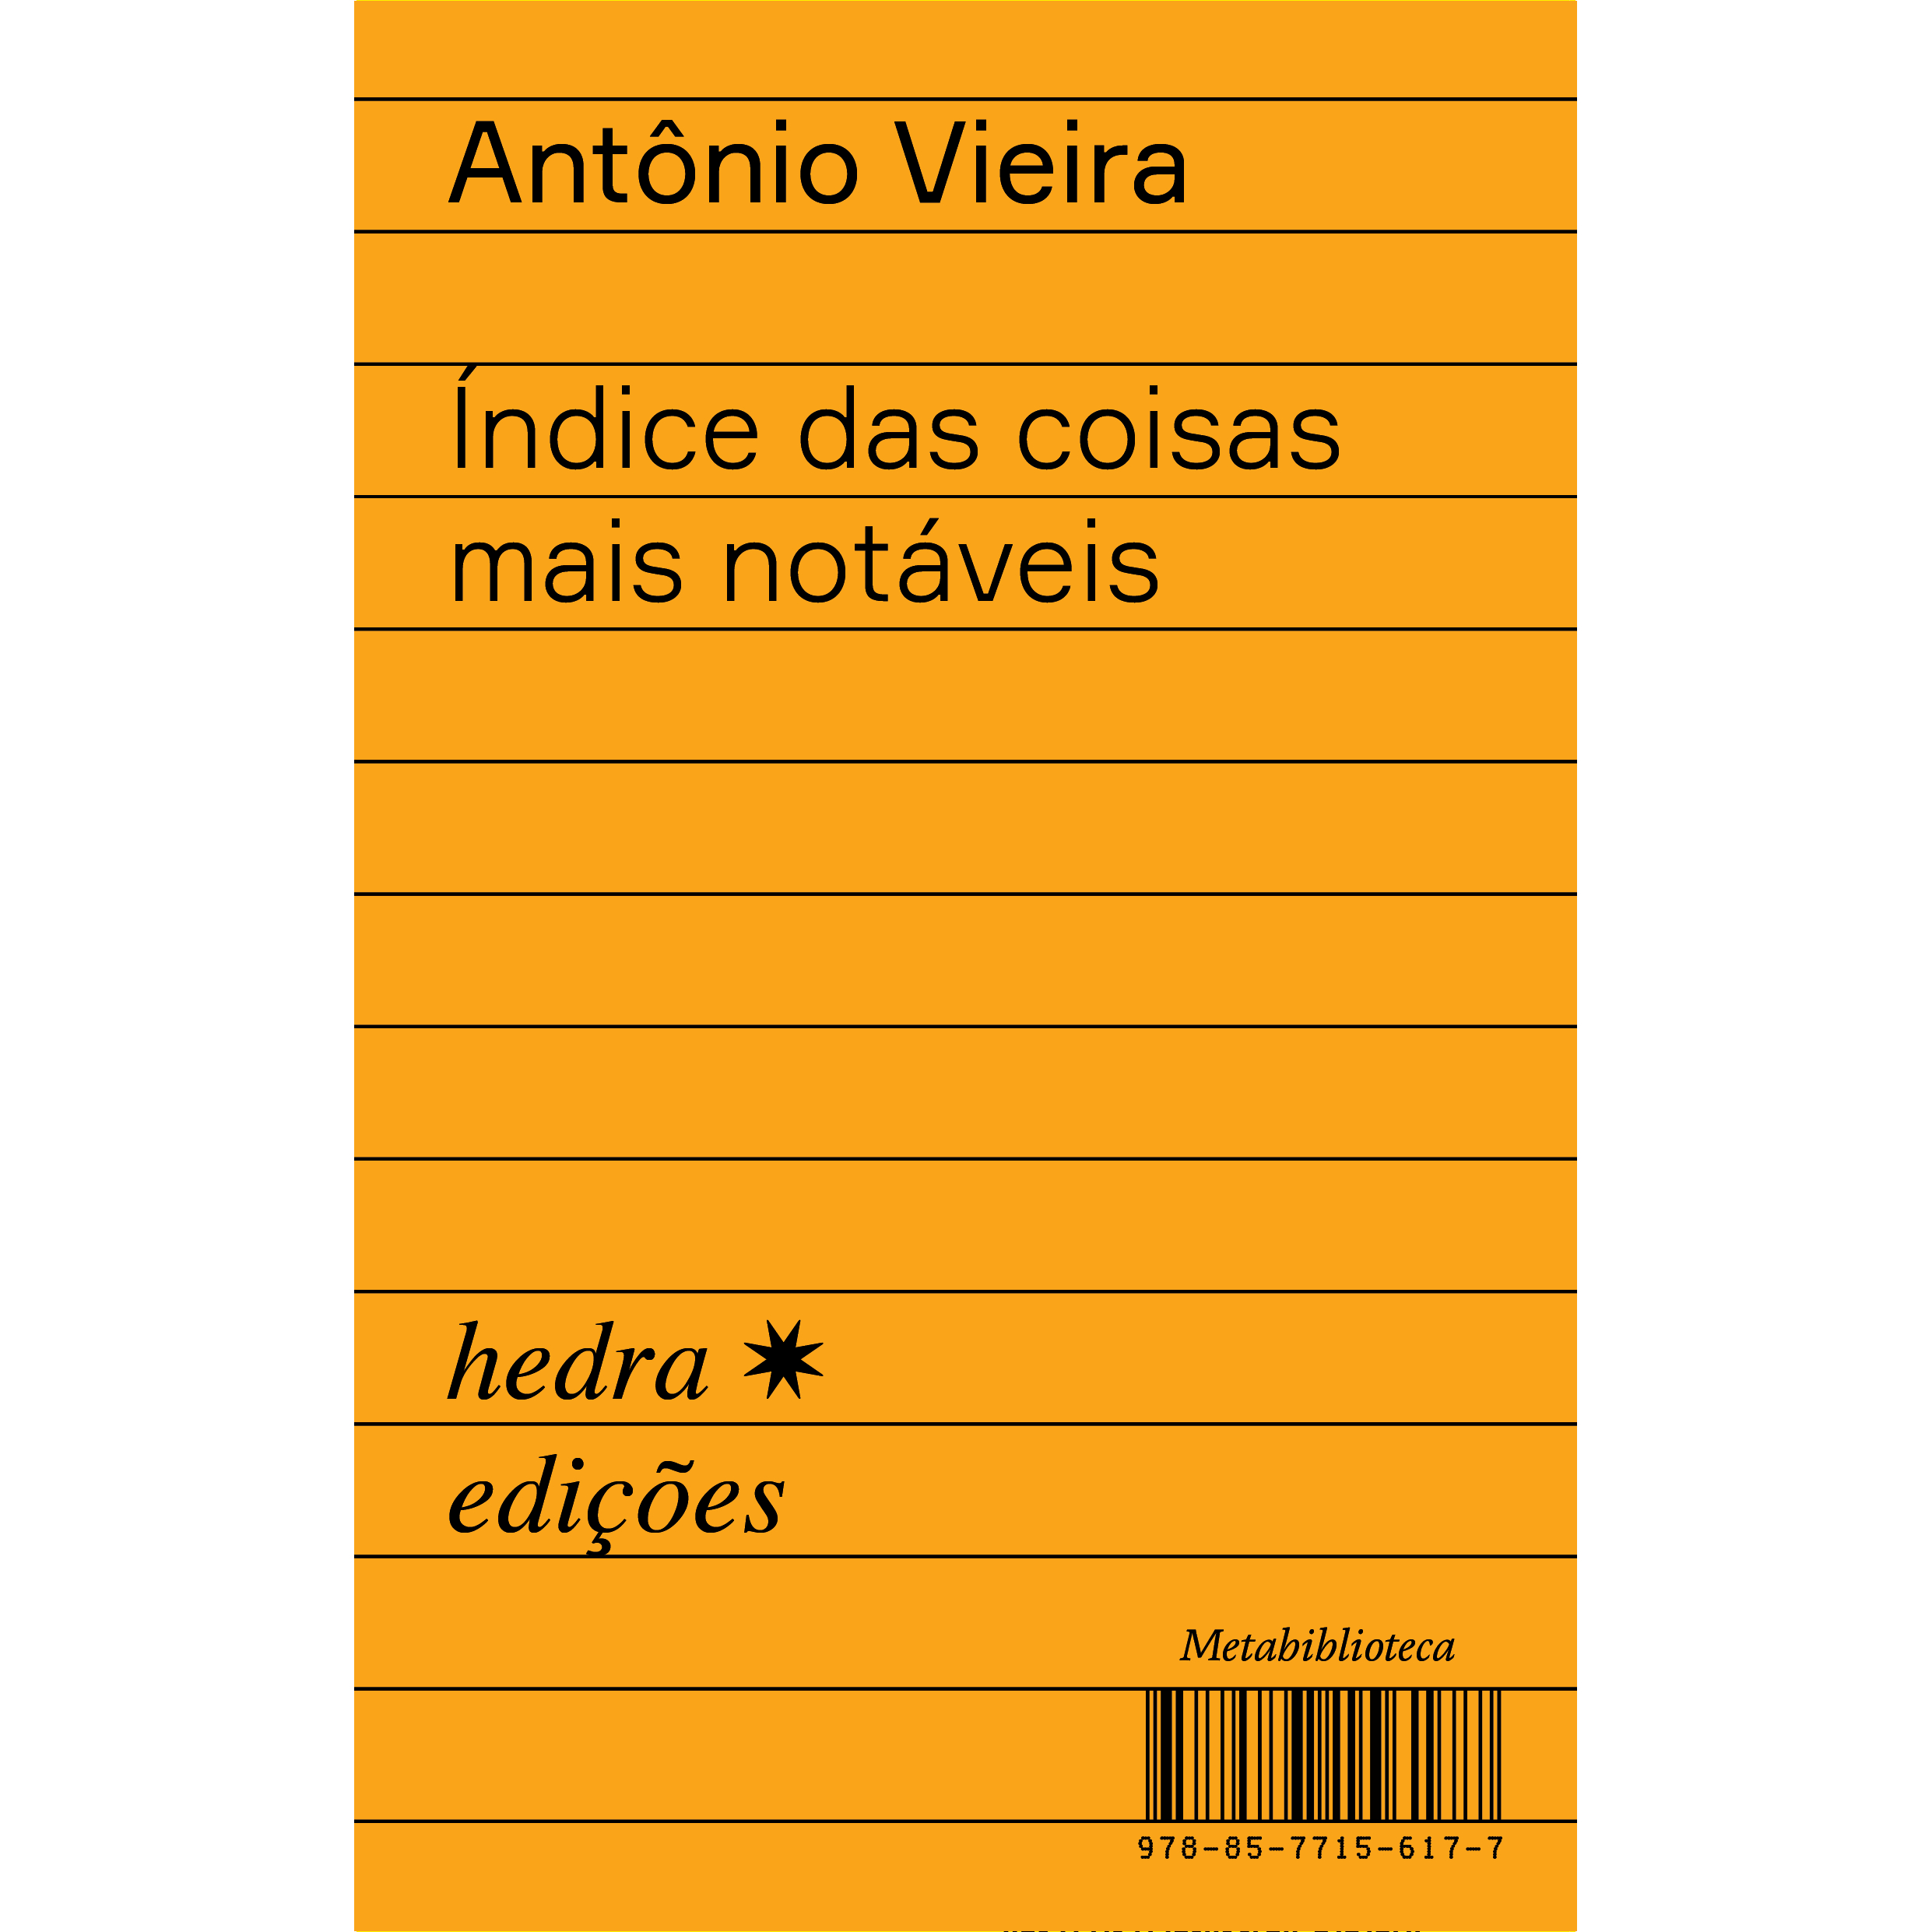
\includegraphics[width=92mm]{./grid/vieira.jpg}
\end{center}

\hspace*{-7cm}\hrulefill\hspace*{-7cm}

\medskip

\noindent{}{\slsc{Índice das coisas mais notáveis}} reúne os glossários de frases produzidos como apêndices para a primeira edição dos {\slsc{Sermões}}, publicados em 15
volumes durante os anos 1679 e 1748. Com exatamente 1178 verbetes,
sem repetição, para um total de 8364 frases de abonação extraídas do corpo dos
{\slsc{Sermões}}, a obra permite uma visão sintética, articulada e complexa do léxico de
Vieira e, por extensão, de todo o léxico intelectual do século \scalebox{.8}{XVII}
português.

Os verbetes, que mantêm a unidade
teológico"-retórico"-política dos {\slsc{Sermões}}, podem ser divididos em quatro
grupos, e lidos, portanto: (a) como repertório da \textit{invenção} dos argumentos da
tradição do gênero da oratória sacra glosados pelos sermões vieirianos; (b)
como coletânea de enunciados lapidares, análogos a \textit{sentenças} e
\textit{máximas} morais; (c) como \textit{ilustração} ou explicação das
principais categorias tratadas no livro, segundo diferentes tipos de ouvintes
retoricamente previstos nos \textit{Sermões}; (d) como \textit{apologia} das
posições polêmicas adotadas a propósito de várias matérias, de maior ou menor
gravidade, ao longo dos volumes.

\vfill

\hspace*{-.4cm}\begin{minipage}[c]{.5\linewidth}
\small{
{\Formular{\textbf{
\hspace*{-.1cm}Título: Índice das coisas mais notáveis\\
Autor: Antonio Vieira\\ 
ISBN: 978-85-7715-646-7\\
Páginas: ???\\
Formato: 13,3x21cm\\
Preço: R\$ ????\\
Editora: Hedra\\
Disponibilidade: 31/07/2020
}}}}
\end{minipage}

\pagebreak

\hspace{.5cm}

\begin{center}
\hspace*{.5cm}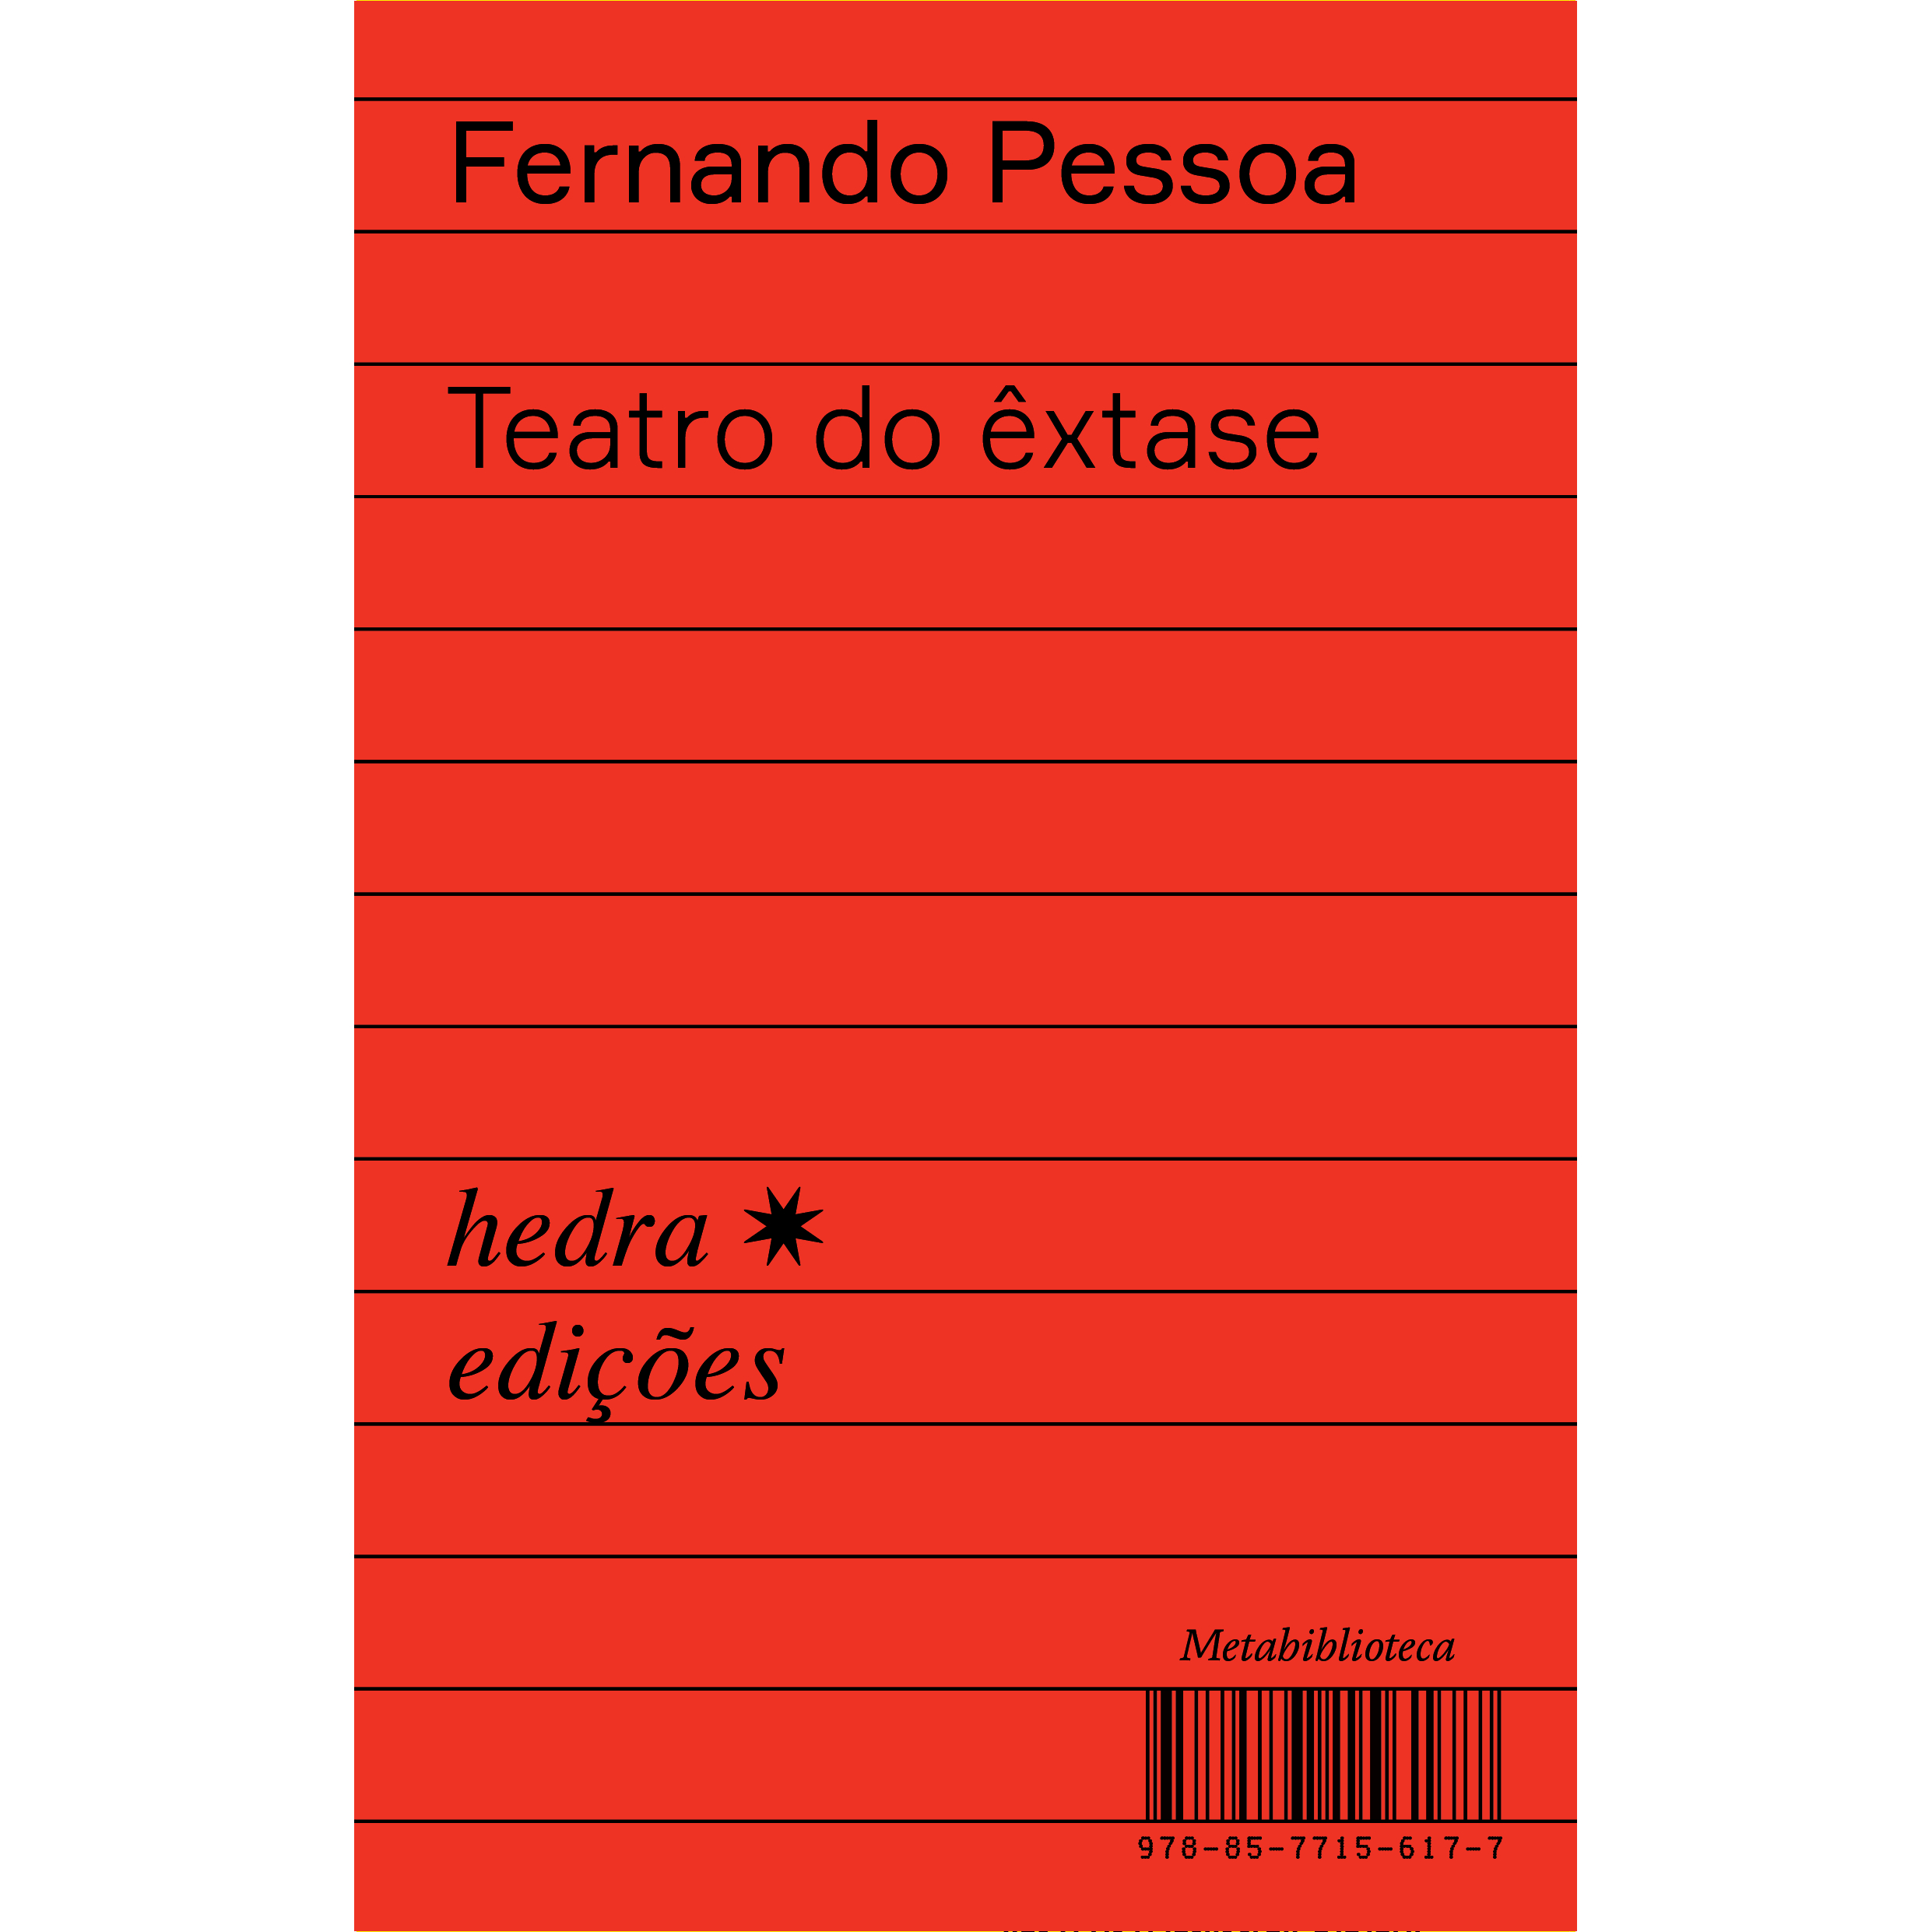
\includegraphics[width=92mm]{./grid/pessoa.jpg}
\end{center}

\hspace*{-7cm}\hrulefill\hspace*{-7cm}

\medskip

\noindent{}{\slsc{Teatro do êxtase}} reúne cinco peças de Fernando Pessoa, concebidas 
como poemas dramáticos e destinadas mais à leitura do que à encenação. 
{\slsc{O marinheiro}} (1915), único drama publicado em vida, foi incluído no
primeiro número da revista {\slsc{Orpheu}} e figura, juntamente com
{\slsc{Fausto}}, como sua peça mais importante.  Definida pelo próprio autor
como um ``drama estático'', a obra de matriz simbolista apresenta o diálogo
entre três mulheres que velam o corpo de uma donzela, sem nenhuma referência
histórica.

Ainda estão aqui reunidos {\slsc{A morte do príncipe}}, que remonta a {\slsc{Hamlet}}, de Shakespeare; {\slsc{Diálogo no jardim do palácio}}, com referências platônicas à reflexão sobre o amor e à dicotomia entre corpo e alma; {\slsc{Salomé}}, leituras do
tema bíblico da {\slsc{mulher fatal}}; e {\slsc{Sakyamuni}}, representação da ascensão de Siddhartha Gautama ao estado de iluminação. Provavelmente as peças mais acabadas do autor, apresentam como eixo comum a concepção pessoana de ``êxtase''. 
%

\vfill

\hspace*{-.4cm}\begin{minipage}[c]{.5\linewidth}
\small{
{\Formular{\textbf{
\hspace*{-.1cm}Título: Teatro do êxtase\\
Autor: Fernando Pessoa\\ 
ISBN: 978-85-7715-647-4\\
Páginas: ???\\
Formato: 13,3x21cm\\
Preço: R\$ ????\\
Editora: Hedra\\
Disponibilidade: 31/07/2020
}}}}
\end{minipage}

\pagebreak


\hspace{.5cm}

\begin{center}
\hspace*{-2.5cm}\raisebox{6.8cm}{\rotatebox[origin=t]{90}{\huge\Formular{\textbf{Lançamento}}}}
\hspace*{2.5cm}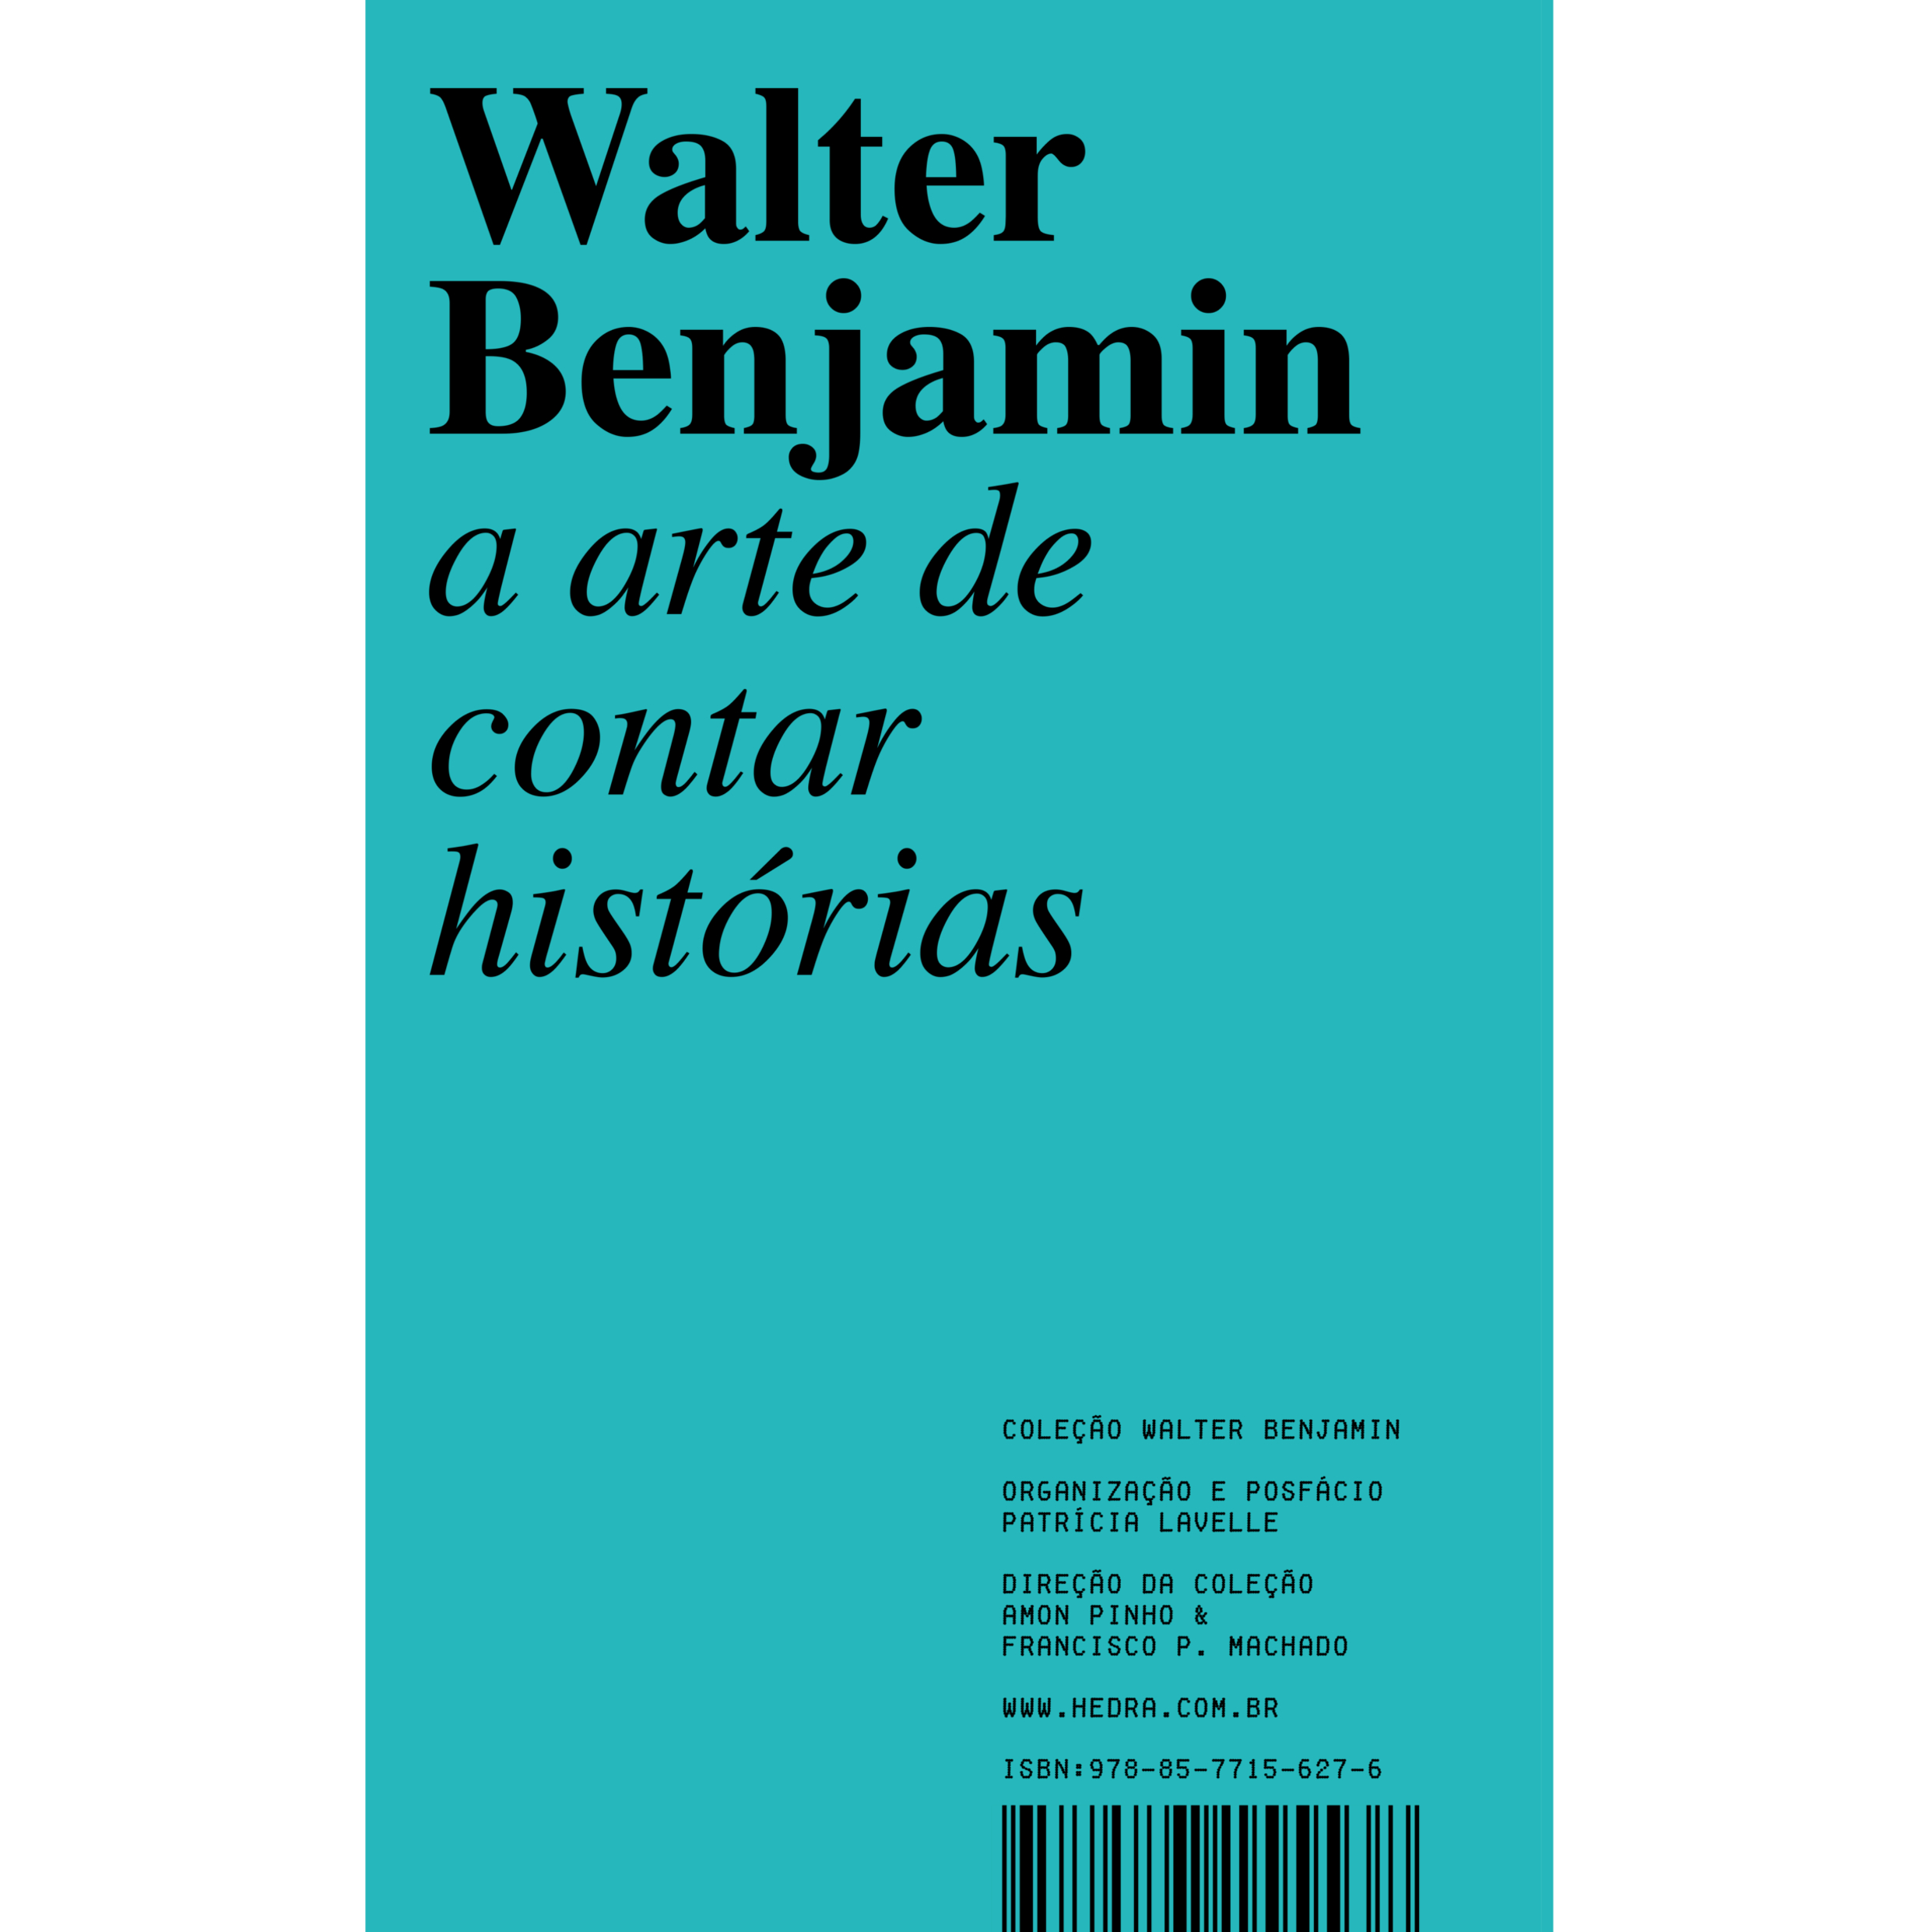
\includegraphics[width=92mm]{./grid/benjamin.jpg}
\end{center}

\hspace*{-7cm}\hrulefill\hspace*{-7cm}

\medskip

\noindent{}{\slsc{A arte de contar histórias}} propõe uma nova tradução anotada do clássico ensaio de Walter Benjamin, no qual apresenta a figura do contador de histórias a partir de um comentário crítico do contista russo Nikolai Leskov. Além do célebre ensaio, ora traduzido como “O narrador”, o livro também reúne sua produção ficcional: quinze contos --- alguns inéditos em português ---, quatro narrativas radiofônicas e quatro textos literário"-críticos.

Escritos entre 1928 e 1936, perpassam uma variedade de questões caras ao pensador, mas marcados sobretudo pela preocupação com o fim da arte de contar histórias. Ademais, os textos desta edição convidam o leitor a pensar a relação de oposição entre filosofia e literatura, conduzindo ao entrecruzamento dessas duas formas de discurso. Benjamin foi ensaísta, crítico literário, tradutor, sociólogo, tradutor (de Baudelaire, Proust e Balzac, entre outros) e filósofo, ligado à Escola de Frankfurt. Entre seus interlocutores e amigos, encontram"-se personalidades marcantes do século \scalebox{.8}{XX} como Adorno, Hannah Arendt, Brecht e Gershon Scholem.

%\hspace{.5cm}
\vfill

\hspace*{-.4cm}\begin{minipage}[c]{.5\linewidth}
\small{
{\Formular{\textbf{
\hspace*{-.1cm}Título: A arte de contar histórias [2ª edição]\\
Autor: Walter Benjamin\\ 
ISBN: 978-85-7715-627-6\\
Páginas: 288\\
Formato: 13,3x21cm\\
Preço: R\$ 50\\
Editora: Hedra\\
Disponibilidade: 28/08/2020
}}}}
\end{minipage}


\pagebreak

\hspace{.5cm}

\begin{center}
\hspace*{.5cm}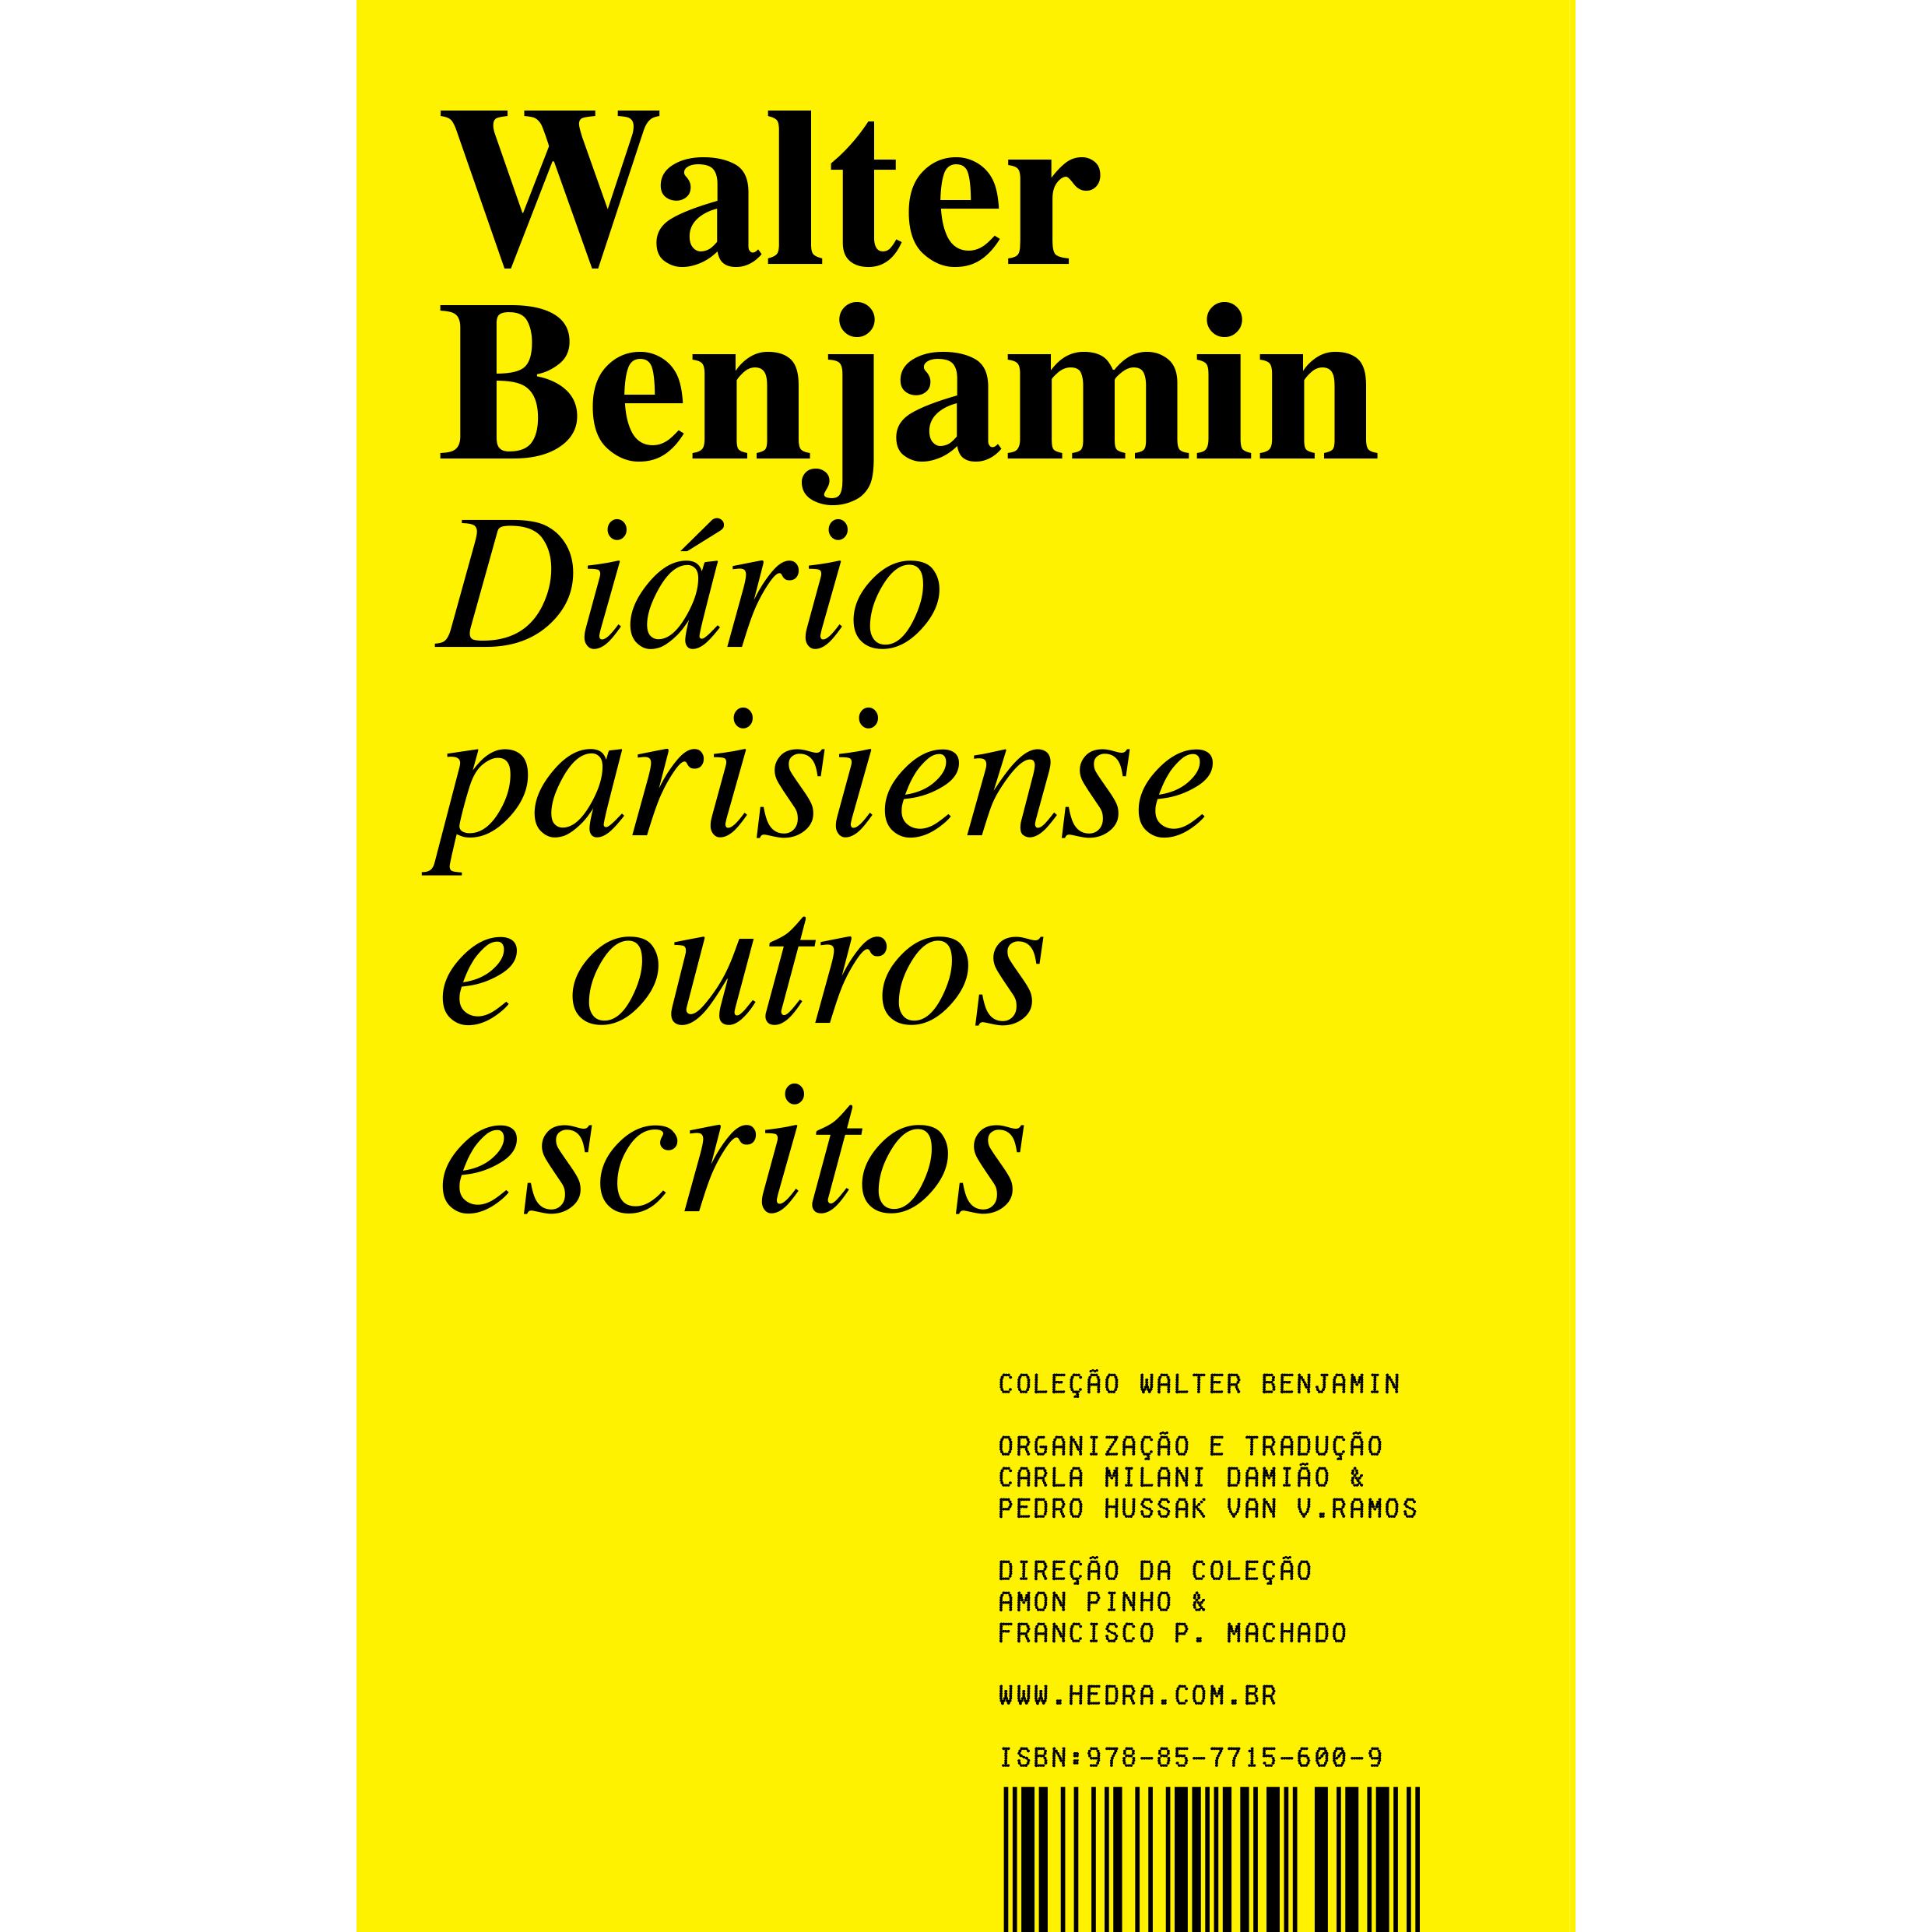
\includegraphics[width=92mm]{./grid/benjamin2.jpg}
\end{center}

\hspace*{-7cm}\hrulefill\hspace*{-7cm}

\medskip

\noindent{}{\slsc{Diário parisiense e outros escritos}} reúne quinze textos de Walter Benjamin de 1926 a 1936, enquanto viveu na França --- dentre eles seu próprio diário escrito entre 1929 e 1930, que dá nome ao livro, é e inédito em português. A seleta de textos remete também ao trânsito entre Alemanha e França percorrido por Benjamin, em vários sentidos: literário"-crítico, filosófico, artístico, político e biográfico. Nesse trânsito, procuramos pelo “lugar” de Benjamin, como um crítico literário exemplar, judeu"-alemão e refugiado político, inserido no debate literário francês no período entreguerras.

O volume também apresenta as suas análises dos que considerava principais nomes da literatura francesa: Gide, Valéry e Proust. O caráter legítimo ou autêntico de Benjamin como crítico literário, pouco ou nada ortodoxo, tornava os escritores não apenas o objeto de sua crítica literária, mas coautores de um sentido de crítica inusitado. Textos como “Cartas parisienses” também são claros exemplos do lugar político e social que assumia, quando exigia"-se dos intelectuais um posicionamento em face do tempo em que viviam.

%\hspace{.5cm}
\vfill

\hspace*{-.4cm}\begin{minipage}[c]{.5\linewidth}
\small{
{\Formular{\textbf{
\hspace*{-.1cm}Título: Diário parisiense e outros escritos\\
Autor: Walter Benjamin\\ 
ISBN: 978-85-7715-600-9\\
Páginas: 244\\
Formato: 13,3x21cm\\
Preço: R\$ ?????\\
Editora: Hedra\\
Disponibilidade: 28/08/2020
}}}}
\end{minipage}

\pagebreak



\hspace{.5cm}

\begin{center}
\hspace*{-2.5cm}\raisebox{6.8cm}{\rotatebox[origin=t]{90}{\huge\Formular{\textbf{Lançamento}}}}
\hspace*{2.5cm}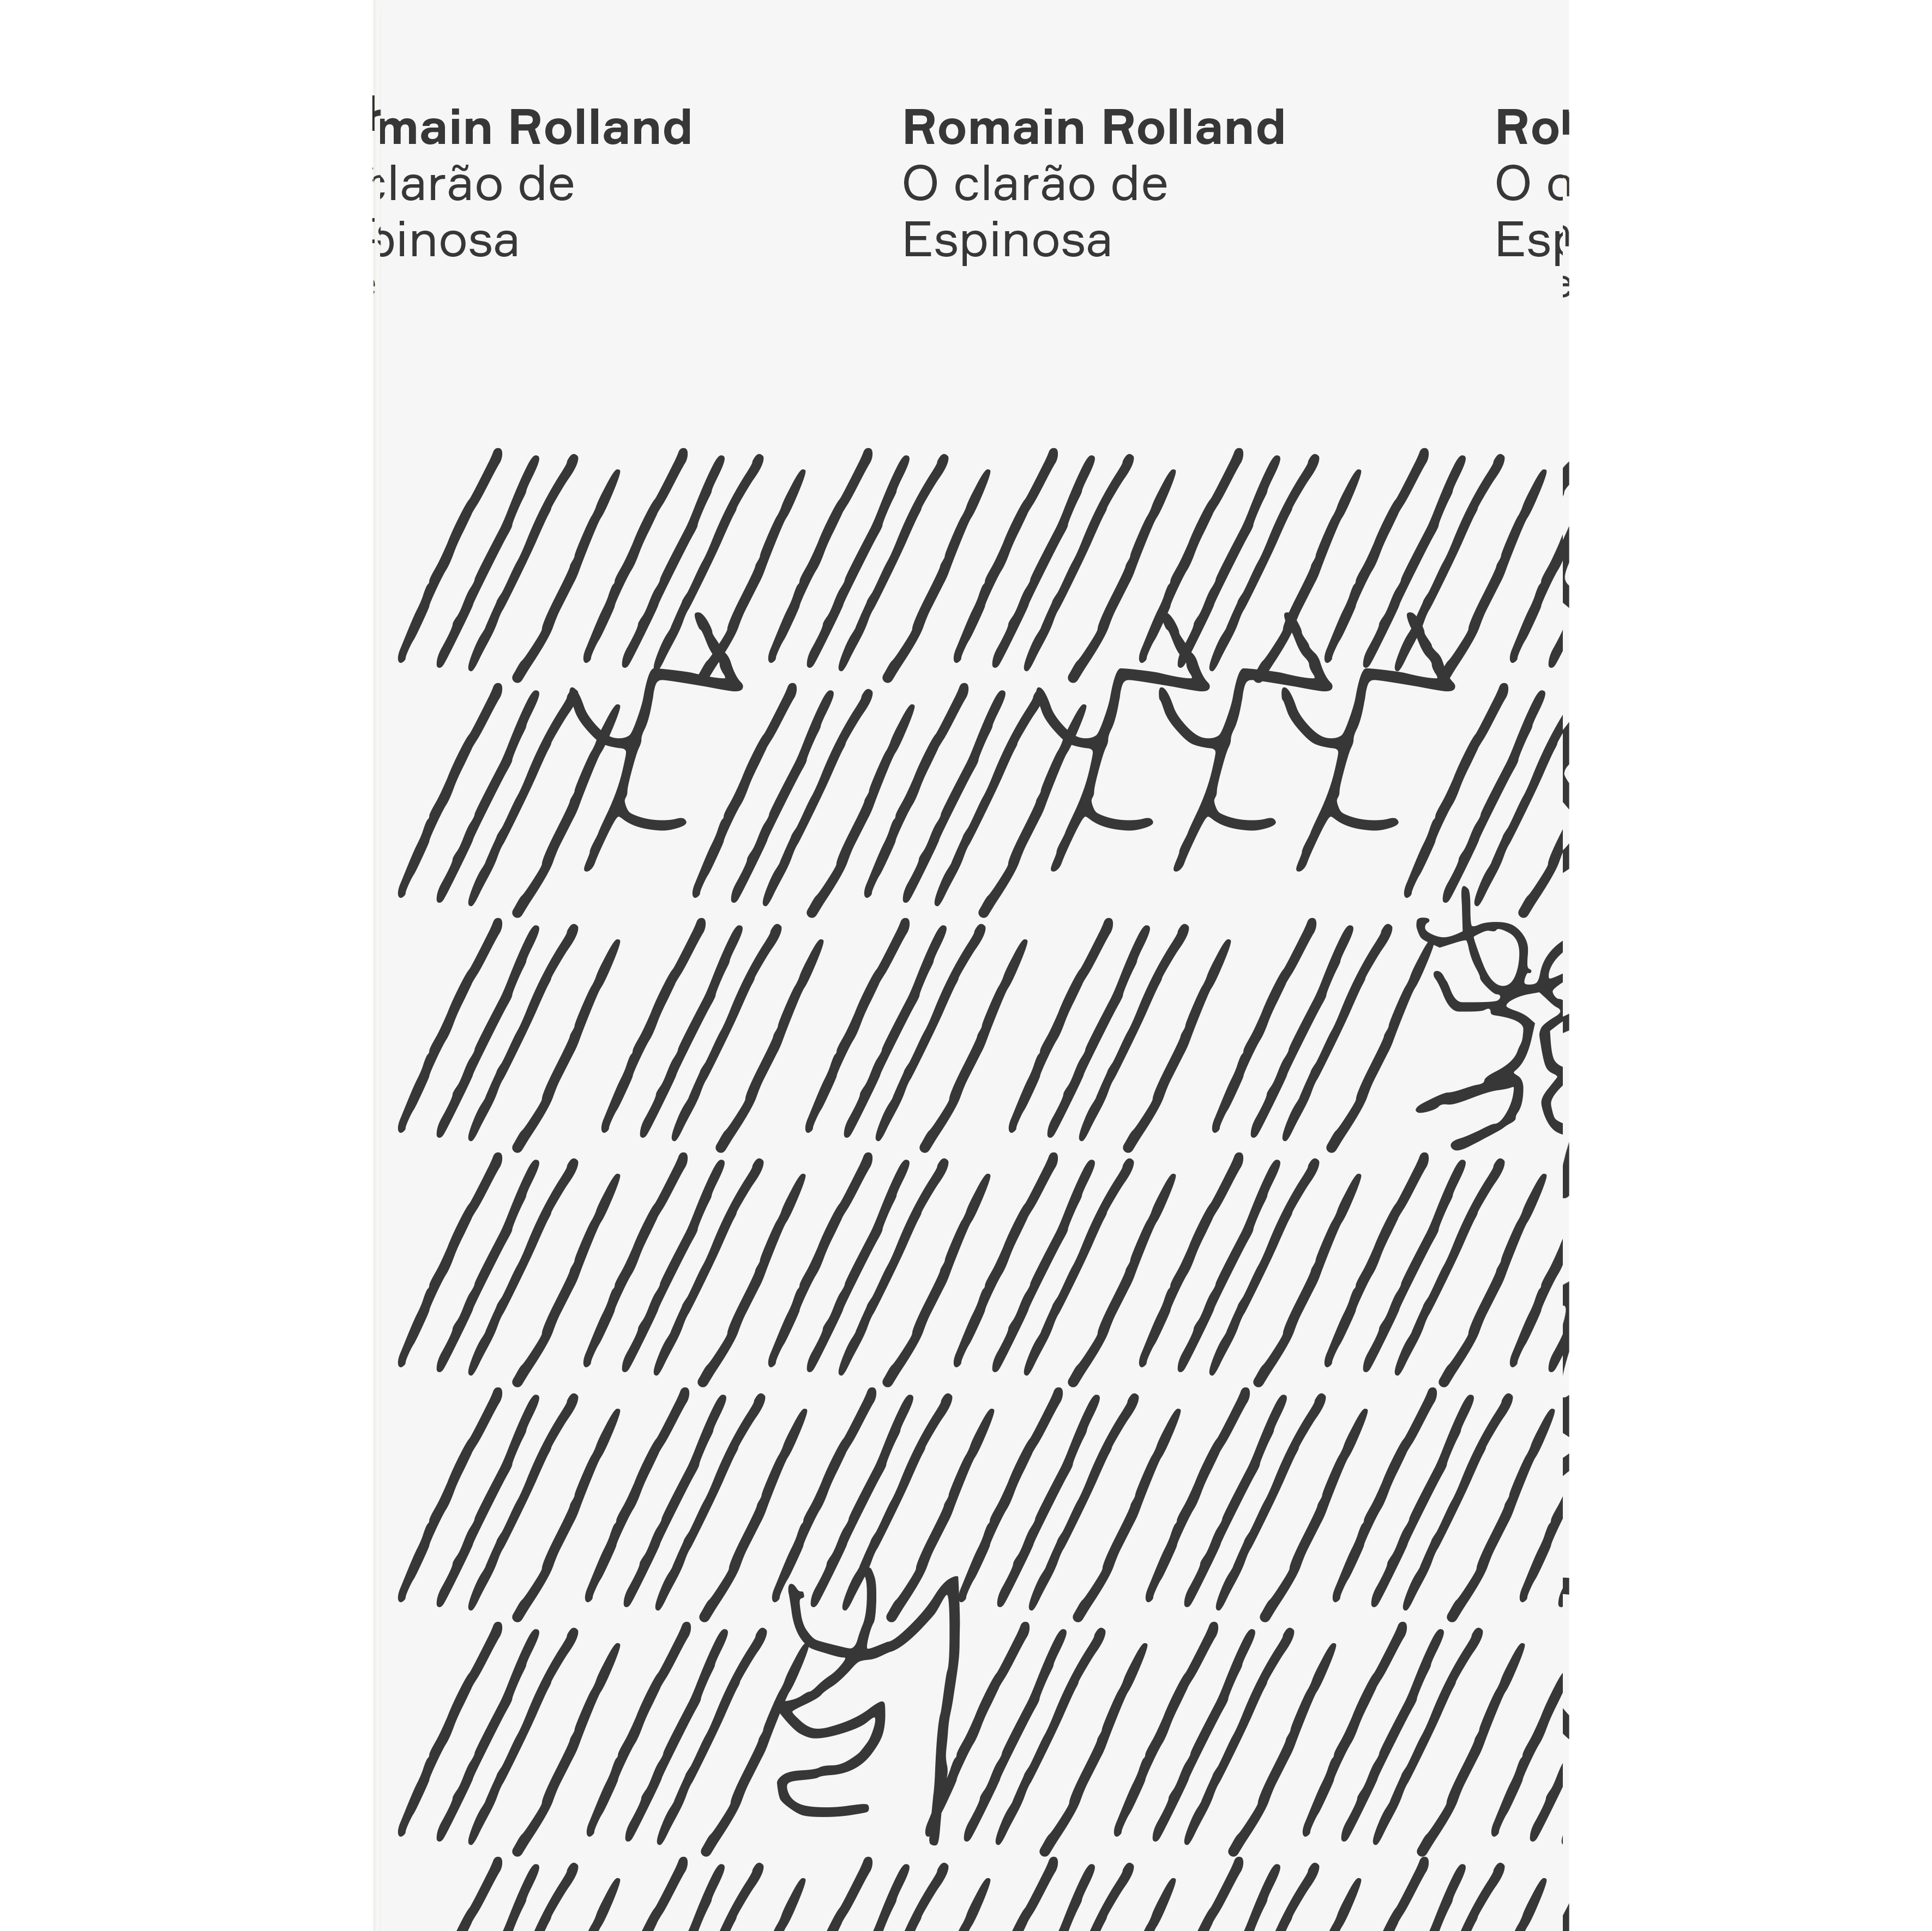
\includegraphics[width=92mm]{./grid/rolland.png}
\end{center}

\hspace*{-7cm}\hrulefill\hspace*{-7cm}

\medskip

\noindent{}Romain Rolland foi novelista, biógrafo, músico e Nobel francês de 1915. Escreveu as presentes páginas sobre Espinosa, repletas de lirismo e potência filosófica, ainda na adolescência, mas foram publicadas apenas em 1942 no livro {\slsc{A viagem interior}}. Neste livro o jovem Rolland conta o “clarão” que teve em sua vida ao ler Espinosa pela primeira vez aos 16 anos, e como isso definiu sua vida e carreira.

Em cuidadosa edição bilíngue, o leitor aproxima"-se dos movimentos luminosos do texto original. O livro é marcado por uma linguagem fremente e impressionista, que segue rente à experiência de deslumbre e atordoamento de Rolland diante da leitura do filósofo. Por trás das imagens poéticas, vislumbra"-se ainda um questionamento existencial e ontológico da condição humana --- reminiscências da filosofia de Espinosa no pensamento e em sua própria prosa. Como escreve o autor, a leitura de Espinosa foi um “desses jatos da alma, desses clarões, que inundaram minhas veias com o fogo que faz bater o coração do universo”. Às “palavras de fogo de Espinosa” dedica"-se esse relato.

\vfill

\hspace*{-.4cm}\begin{minipage}[c]{.5\linewidth}
\small{
{\Formular{\textbf{
\hspace*{-.1cm}Título: O clarão de Espinosa [bilíngue]\\
Autor: Romain Rolland\\ 
ISBN: 978-65-8109-708-0\\
Páginas: 57\\
Formato: 11x18cm\\
Preço: R\$ 29,90\\
Editora: Hedra \& n-1\\
Disponibilidade: 11/09/2020
}}}}
\end{minipage}

\pagebreak

\hspace{.5cm}

\begin{center}
\hspace*{.5cm}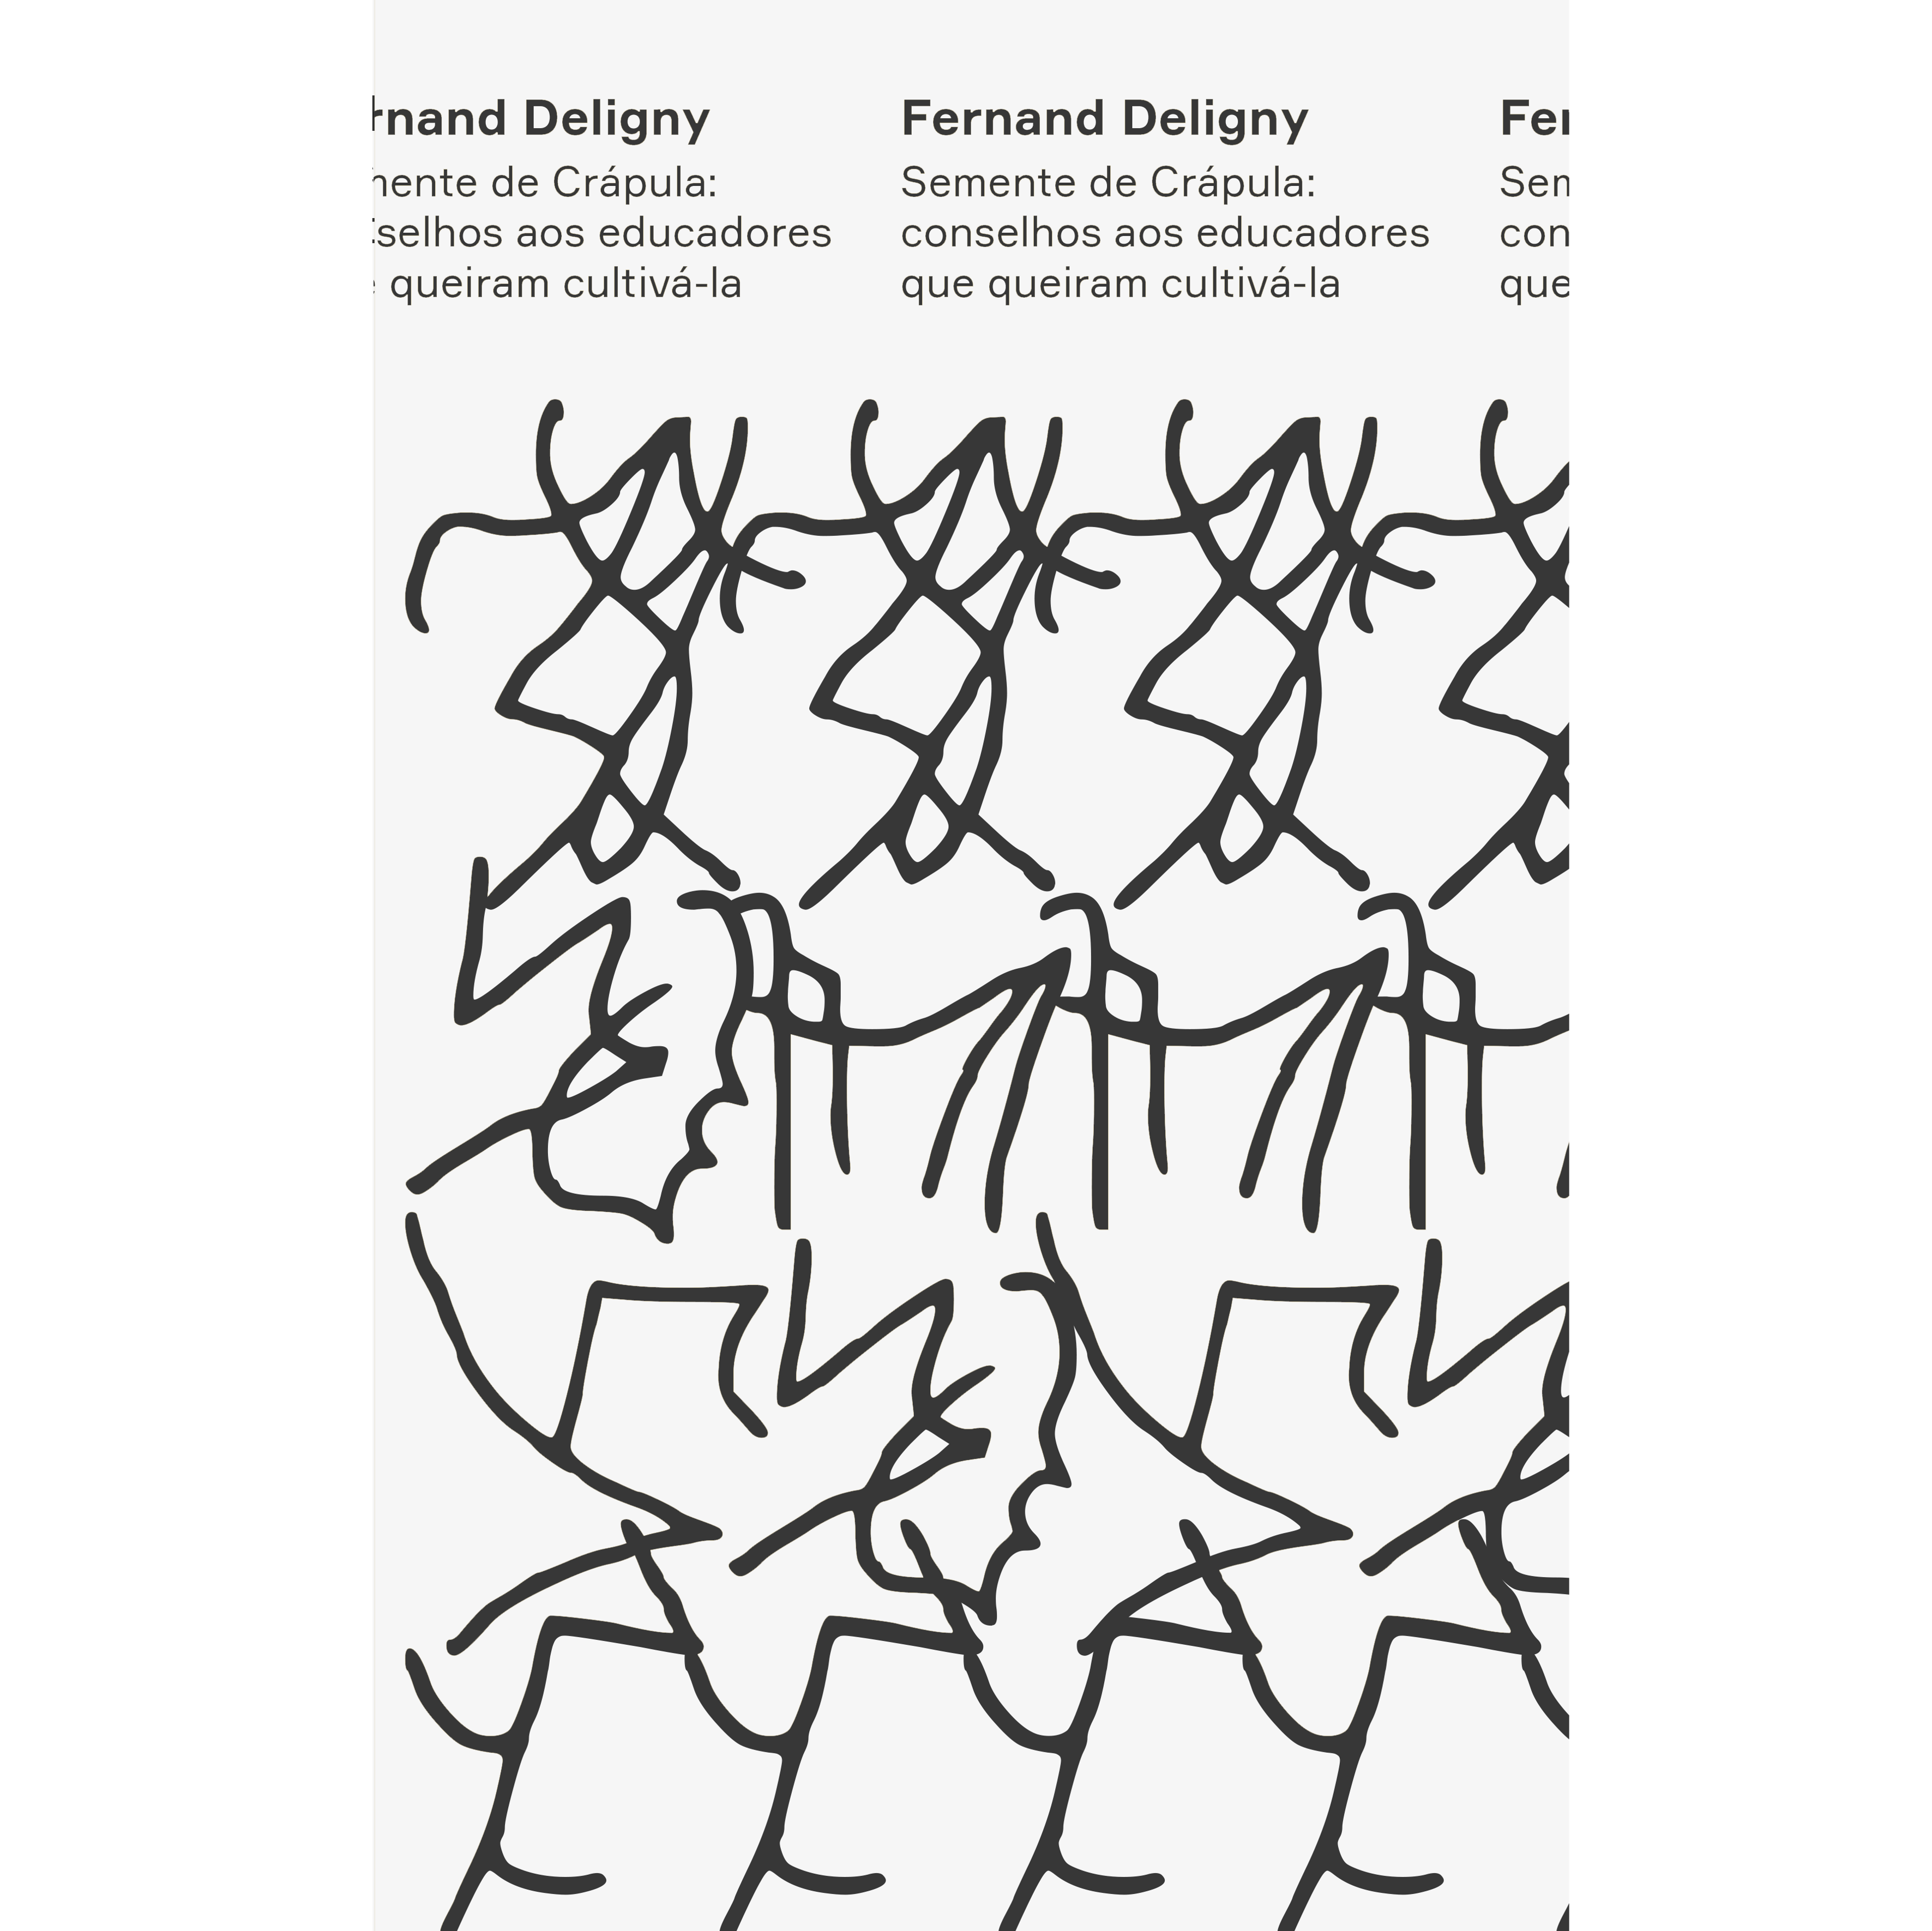
\includegraphics[width=92mm]{./grid/deligny.png}
\end{center}

\hspace*{-7cm}\hrulefill\hspace*{-7cm}

\medskip

\noindent{}{\slsc{Semente de crápula: conselhos aos educadores que queiram cultivá-la}} é o primeiro livro do educador e poeta francês Fernand Deligny. É um balizador de seu trabalho, que o situaria como uma das maiores referências da educação especial --- lidando com crianças e jovens psicóticos, delinquentes, “perigosos”, “marginais” --- e da pedagogia em geral.

Ao longo dos 134 aforismos, Deligny apresenta suas “sementes”: jovens de um meio social delinquente, cultivadas pelo educador que deve deixar de lutar contra as ervas daninhas, pragas sociais atadas ao nosso convívio social, para mergulhar nas dinâmicas espaciais desses jovens que criam outros sentidos de lugar e convivência no território. Publicado em 1945, o livro foi rapidamente bem sucedido na França por sua linguagem poética simples e a franqueza do autor. Deligny passou os primeiros vinte anos de atuação profissional entre escolas especiais, instituições médico"-pedagógicas e hospitais psiquiátricos.

\vfill

\hspace*{-.4cm}\begin{minipage}[c]{.5\linewidth}
\small{
{\Formular{\textbf{
\hspace*{-.1cm}Título: Semente de crápula — conselhos\\ aos educadores que queiram cultivá-la\\
Autor: Fernand Deligny\\ 
ISBN: 978-65-8109-709-7\\
Páginas: 96\\
Formato: 11x18cm\\
Preço: R\$ 34,90\\
Editora: Hedra \& n-1\\
Disponibilidade: 11/09/2020
}}}}
\end{minipage}

\pagebreak

\hspace{.5cm}

\begin{center}
\hspace*{-2.5cm}\raisebox{6.8cm}{\rotatebox[origin=t]{90}{\huge\Formular{\textbf{Lançamento}}}}
\hspace*{2.5cm}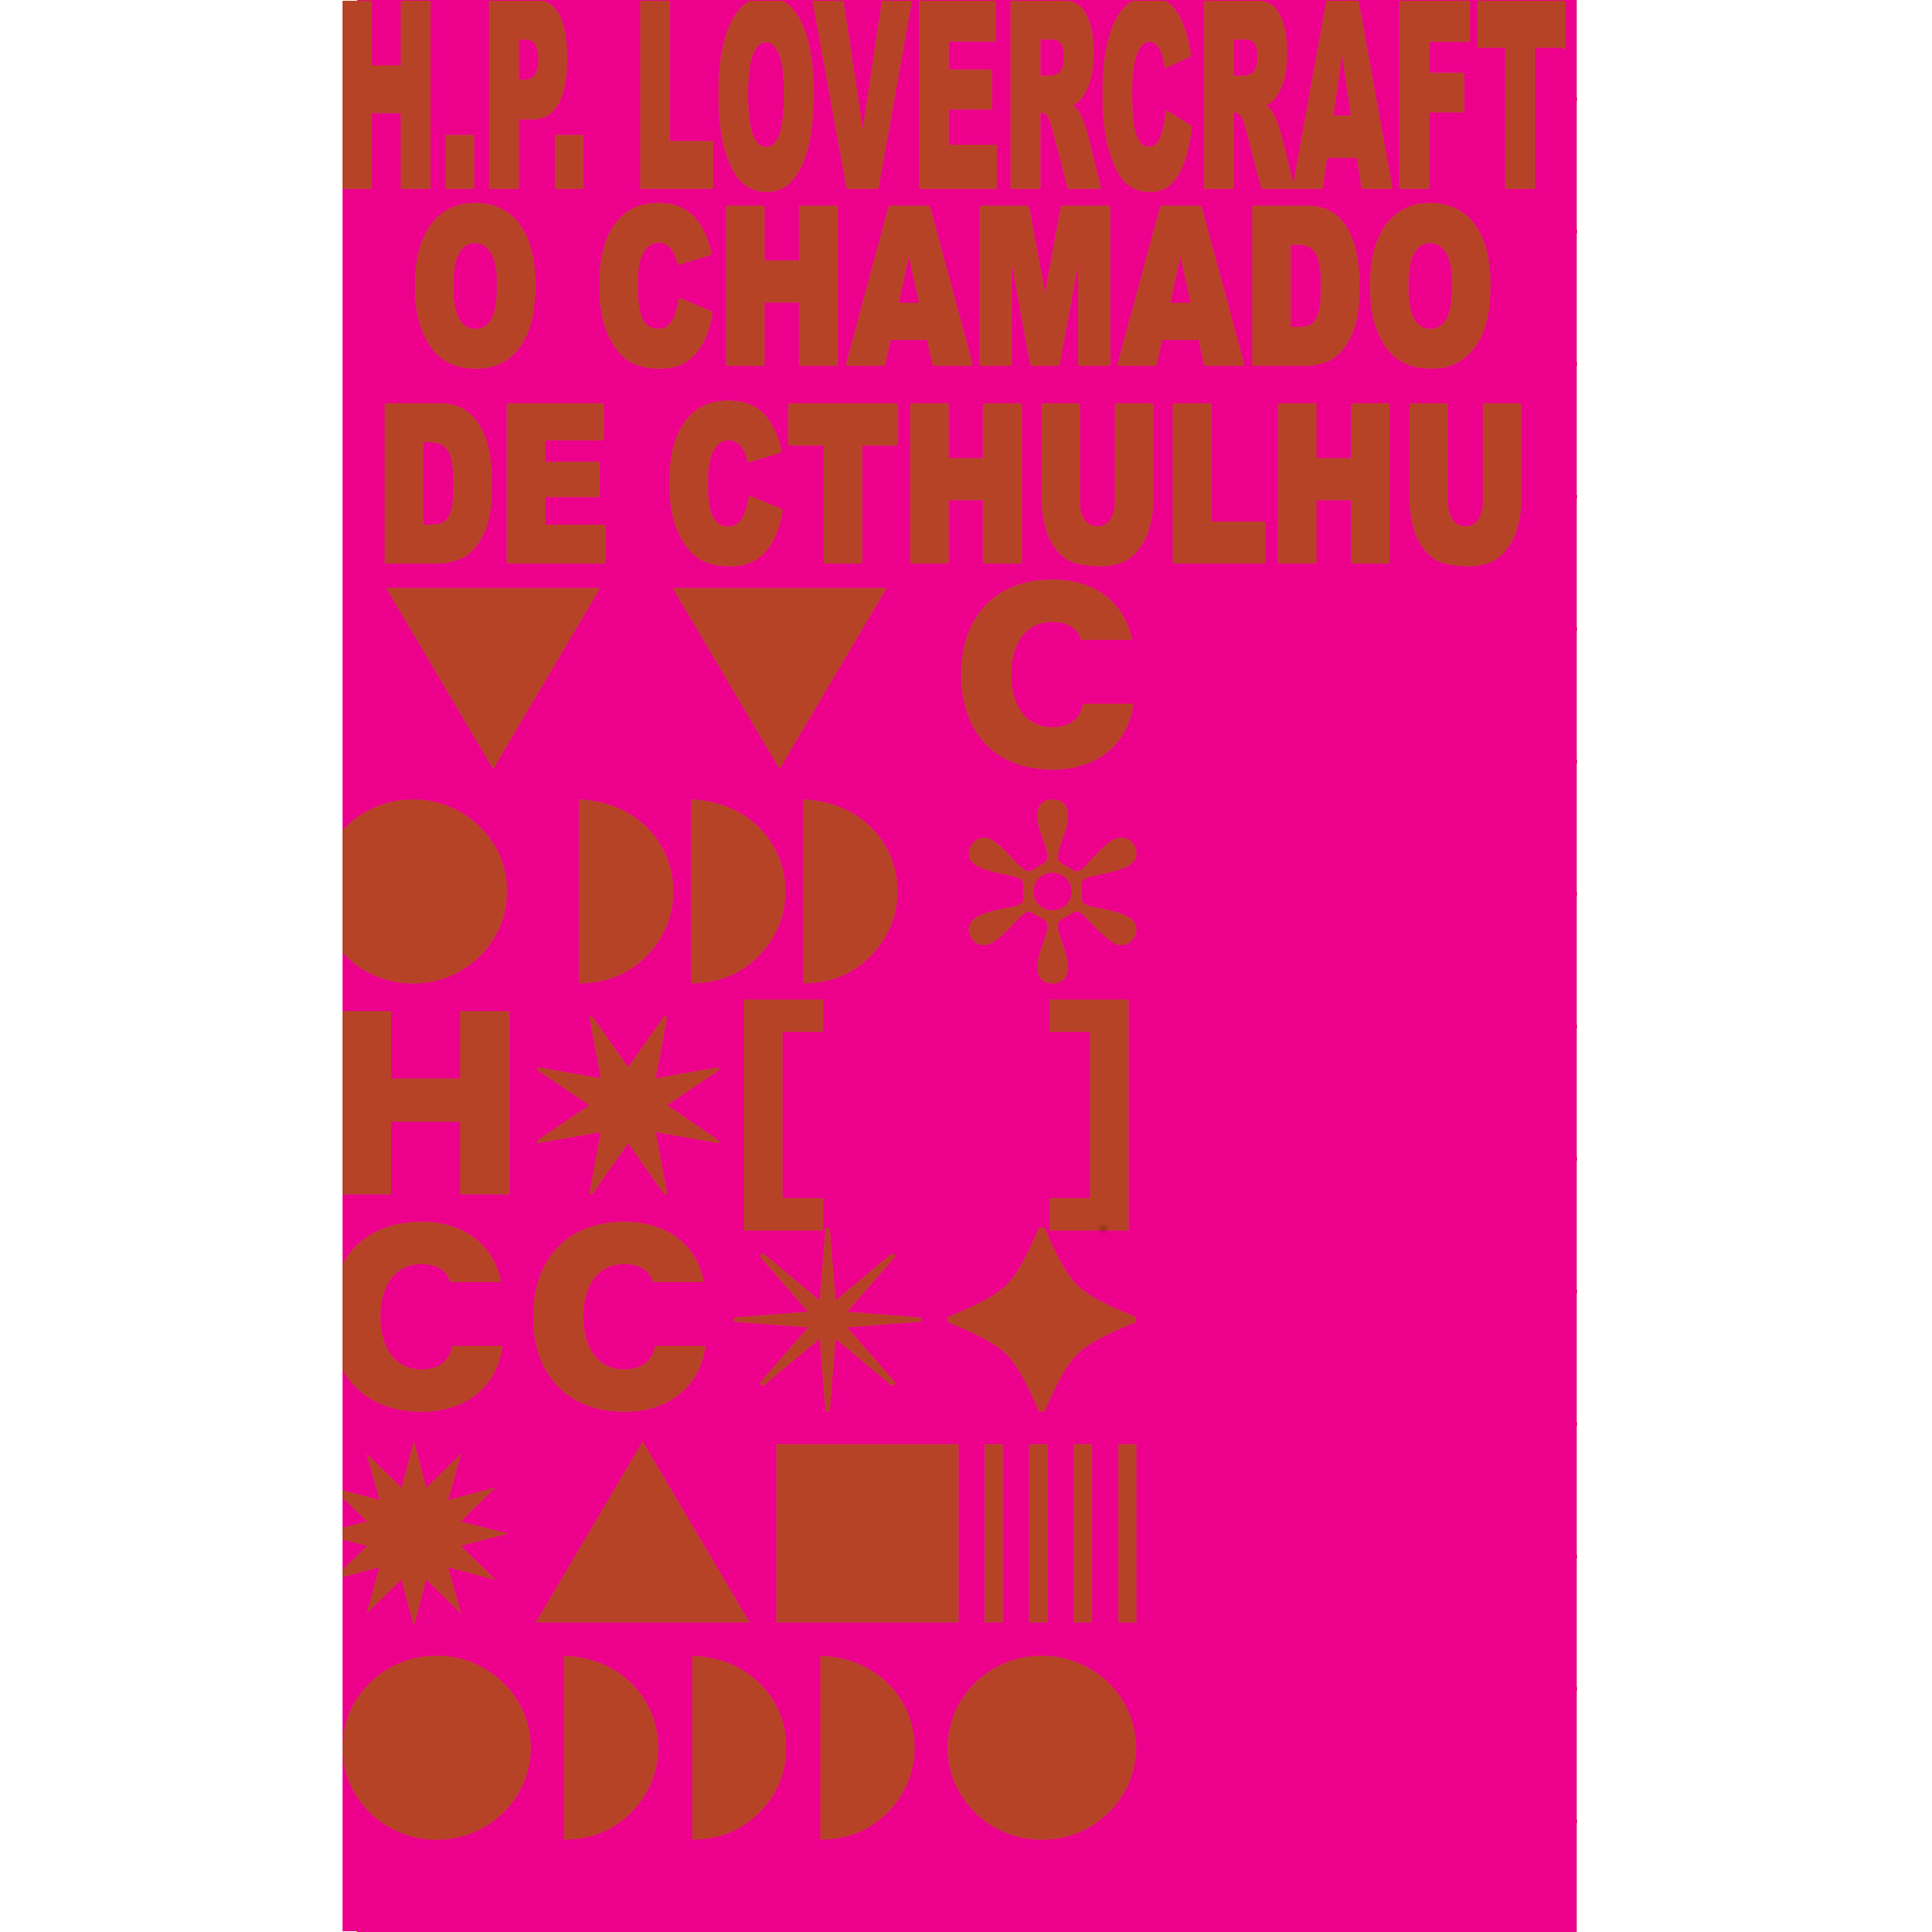
\includegraphics[width=92mm]{./grid/lovecraft.jpg}
\end{center}

\hspace*{-7cm}\hrulefill\hspace*{-7cm}

\medskip

\noindent{}{\slsc{O chamado de Cthulhu}} reúne narrativas escritas ao longo de toda a vida de H.P. Lovecraft, desde a sua estreia literária (“Dagon”) até obras concluídas pouco antes de sua morte (“O assombro das trevas”). Também integram a seleção
“O chamado de Cthulhu”, um dos grandes clássicos de horror do século \scalebox{.8}{XX}, e o inedito “A música de Erich Zann”, considerado pelo próprio autor um de seus melhores escritos.

Ao fim do volume, o leitor encontrará no apêndice uma carta escrita por
Lovecraft ao amigo R. Michael, em que fala sobre sua personalidade e sua vida, e um artigo em que discute o método que empregava na criação de seus contos fantásticos. {\slsc{O
chamado de Cthulhu e outros contos}} é um desconcertante passeio pelo universo macabro de um dos grandes mestres do horror.

\vfill

\hspace*{-.4cm}\begin{minipage}[c]{.5\linewidth}
\small{
{\Formular{\textbf{
\hspace*{-.1cm}Título: O chamado de Cthulhu\\
Autor: H. P. Lovecraft\\ 
ISBN: 978-85-7715-648-1\\
Páginas: ???\\
Formato: 13,3x21cm\\
Preço: R\$ ????\\
Editora: Hedra\\
Disponibilidade: 11/09/2020
}}}}
\end{minipage}

\pagebreak

\begin{changemargin}
\hspace{.5cm}
\vspace*{1cm}
\enlargethispage{-\baselineskip}

\noindent{}{\LARGE{Como o horror cósmico de H.\,P. Lovecraft dominou a cultura pop\\{\large\slsc{Obras do escritor inspiram cada vez mais livros, filmes, quadrinhos e videogames}}}}

\medskip

\hfill{}\scalebox{.8}{ANDRÉ CÁCERES}

\bigskip

Depois de morrer, H.\,P. Lovecraft se tornou uma de suas criações: aterrorizante, onipresente, imortal. O escritor americano espreita as mais variadas mídias, da literatura aos quadrinhos, do cinema aos videogames. Morto precocemente aos 46 anos, o criador do horror cósmico parece ter se erguido do túmulo como Cthulhu, uma das entidades presentes em seus contos, para reclamar o que lhe é de direito.

“A fortuna crítica sobre ele cresce a olhos vistos no Brasil”, afirma ao {\slsc{Estado}} o professor Caio Alexandre Bezarias, pesquisador de Lovecraft. Para ele, o crescente interesse advém do fato de sua obra “expressar como nenhum autor o sentimento de horror perante à pequenez de nossa existência e de como o universo é, não caótico ou hostil, mas indiferente a nós”. 

Essa noção, ele diz, é a pedra fundamental do subgênero que Lovecraft pavimentou. “O leitor neófito deve, ao ler pela primeira vez seus textos, compreender o que é o horror cósmico: a mera revelação do estatuto da nossa espécie no cosmos e que as forças que o governam são totalmente indiferentes a nós causa um horror paralisante.”

Nos últimos tempos, seu universo ficcional inspira todo tipo de adaptação ou releitura. O canal pago \scalebox{.8}{HBO} anunciou a produção de uma série dirigida por Jordan Peele (“Corra!” e “Us”) baseada em {\slsc{Território Lovecraft}} (Intrínseca), de Matt Ruff, que reformula suas lendas e está sendo publicado no Brasil este mês. Releitura semelhante é feita por Victor Lavalle em {\slsc{A Balada do Black Tom}} (Morro Branco), que filtra o racismo inerente à obra lovecraftiana. Já o escritor brasileiro Alexandre Callari, em {\slsc{A Floresta das Árvores Retorcidas}} (Pipoca \& Nanquim), transpõe os mitos de Lovecraft para a realidade brasileira numa cidade pitoresca no interior de São Paulo. 

A \scalebox{.8}{HQ} {\slsc{Os Mitos de Cthulhu}} (Pipoca \& Nanquim), do espanhol Esteban Maroto, adaptação de três contos de Lovecraft, foi publicada recentemente no Brasil. No cinema, o diretor Richard Stanley dirige, com Nicholas Cage, uma versão de {\slsc{A Cor Vinda do Espaço}}, em que um meteoro misterioso cai em uma fazenda e provoca o aparecimento de aberrações e muito além da compreensão humana. Já nos games, a quantidade de jogos inspirados nesses mitos é tamanha que a loja online {\slsc{Steam}} tem a categoria “Lovecraftian Games”, que lista centenas de títulos, como {\slsc{The Sinking City}} (2019) e {\slsc{The Call of Cthulhu}} (2018). 

Para o poeta Dirceu Villa, que está preparando uma nova tradução de sua obra, se Lovecraft escrevesse ensaios, seria acusado de ser um teórico da conspiração, mas sua prosa de ficção fez com que ele transformasse seus preconceitos em metáforas. “Lovecraft era de extrema direita, carregado de preconceitos e ódios profundos, que produziam uma galeria infinita de fantasmas. Era um homem com medo de tudo, das mulheres, de outras etnias, da vida em sociedade”, analisa. “Outras culturas lhe pareciam inferiores e submetidas a coisas sombrias e arcanas, e a sociedade lhe parecia uma farsa grotesca de pessoas inconscientes, e isso tudo lhe deu imagens muito concretas.” O tradutor Alexandre Barbosa de Souza, que verteu alguns dos contos do box {\slsc{Os Mitos de Cthulhu}} (Nova Fronteira), crê que seu horror “vem desse universo mais antigo e alienígena que a história humana, cujo horizonte final é a aniquilação cósmica”.

Nas tramas de Lovecraft, é comum que autoridades (cientistas, linguistas, jornalistas, detetives) tentem decifrar os acontecimentos de maneira cética, mas a razão sempre acaba cedendo ao pavor. Afinal, como ele escreve em {\slsc{O Chamado de Cthulhu}}, “vivemos em uma plácida ilha de ignorância em meio aos mares negros do infinito, e não fomos feitos para viajar muito longe.”

Confira abaixo a íntegra das entrevistas com o professor Caio Alexandre Bezarias, o poeta Dirceu Villa e o tradutor Alexandre Barbosa de Souza sobre a obra de H.\,P. Lovecraft e seu impacto na literatura.

\bigskip
\bigskip

\noindent{}{\LARGE{Entrevista: Caio Alexandre Bezarias}}

\bigskip

\noindent{}{\Formular\textbf{Apesar da popularidade de Lovecraft, a fortuna crítica sobre sua obra ainda parece escassa no Brasil. Como é o panorama da crítica lovecraftiana hoje?}}

 A fortuna crítica sobre ele cresce a olhos vistos no Brasil, mas principalmente a acadêmica. Estudos acadêmicos sobre sua obra são feitos por aqui há bem mais de dez anos, mas até 2004/2005 eram poucos e um tanto, digamos, subterrâneos, quase não circulavam fora do ambiente universitário e mesmo dentro deste, eram um tanto restritos. A partir desta data, mais ou menos, houve um crescimento rápido e hoje, conhecer tudo que se escreve sobre ele em língua portuguesa se tornou tarefa bem ampla e demorada (felizmente). Livros não"-acadêmicos, infelizmente, ainda são poucos, mas o {\slsc{corpus}} disponível desse tipo de publicação é bem maior do que quando eu fiz minha pesquisa de mestrado sobre ele. Então, fecho a resposta com a seguinte afirmação: o panorama é promissor, até mesmo empolgante, pesquisas diversas, de várias linhas, o interesse pela obra só cresce, mas o interessado deve se munir de critérios e senso crítico, pois obviamente muita bobagem também é escrita sobre a obra e ele.

\bigskip

\noindent{}{\Formular\textbf{De que forma os mitos se inserem na obra de Lovecraft e como eles se manifestam?}}

Como eu afirmo em minha pesquisa e no livro no qual ela se transformou, os mitos da sua obra são da categoria dos mitos cosmogônicos, ou seja, mitos que fundamentam o universo em questão, estabelecem a ordem cósmica primordial, quais as forças que erigiram o cosmos do caos primordial e assim o mantêm, incluindo a condição humana nesse cosmos, uma condição que os homens não podem e não conseguem superar. Esses mitos cosmogônicos se manifestam em sua obra na forma dos relatos sobre as entidades cósmicas que definiram o universo, sobre os deuses(na verdade, outras entidades cósmicas, incompreensíveis para a limitada mente humana) que  governaram a Terra no passado e pretendem retomá"-la um dia. Descobrir esses relatos e a verdade sobre a pequenez e banalidade da espécie humana é manifestação desses mitos, no corpo das narrativas, que cria o dito horror cósmico e enlouquece e/ou destrói os protagonistas destas.

\bigskip

\noindent{}{\Formular\textbf{Que chave de leitura da obra de Lovecraft você daria para leitores que pretendem começar a conhecer seu universo?}}

O leitor neófito em H.\,P. Lovecraft deve, ao ler pela primeira vez seus textos, compreender o que é o `horror cósmico': a mera revelação do estatuto da nossa espécie no cosmos e que as forças que o governam são totalmente indiferentes a nós causa um horror paralisante. Éuma chave de leitura fundamental, para a devida fruição da obra. Também recomendo vivamente que a leia como todo texto literário deve ser lido: com vagar, atenção, sem pressa, dado que o estilo de Lovecraft é algo pesado, dado a muitos adjetivos e descrições. E que não espere heroísmos dos protagonistas: não há heróis no sentido exato do termo.

\bigskip

\noindent{}{\Formular\textbf{Como Lovecraft influencia a literatura contemporânea?}}

Dadas a circulação cada vez maior da obra, as leituras e apropriações que escapam de generalizações, essa pergunta recebe uma resposta ampla, multifacetada: de várias formas. Influencia a cosmovisão de vários autores, os fundamentos do universo fictício de suas obras, sem influenciar necessariamente seus estilos de escrita; influencia a temática e cenário: muitos e muitos autores se inspiram em ou copiam seus cenários, entidades, muitas vezes os colocando no mundo contemporâneo. E é nesse caso que ocorrem alguns dos mais crassos erros de jornalismo e leitores apressados ou preguiçosos: está à solta uma mania de afirmar que qualquer narrativa de horror é influenciada por ele e e exemplo do horror cósmico. Menos pressa, mais referências sólidas e leitura atenta, por favor! Um resumo simplório: ele influencia a literatura fantástica/de horror contemporânea como um balizador do sentimento de horror perante à pequena de nossa existência e de como o universo é, não caótico ou hostil, mas indiferente a nós. Essa percepção, que ele expressa como nenhum outro autor, pode explicar porque sua obra é cada vez mais popular, tem tanta penetração no imaginário atual e causa tanto fascínio e interesse.

\bigskip
\bigskip

\noindent{}{\LARGE{Entrevista: Dirceu Villa}}

\bigskip

\noindent{}{\Formular\textbf{Como você diria que Lovecraft trabalha o horror de um ponto de vista formal?}}

Lovecraft tinha uma percepção notável, e muito incomum. Era um homem com medo de tudo, das mulheres, de outras etnias, da vida em sociedade, e isso tudo de maneiras muito específicas: a fisiologia do sexo lhe causava desgosto com suas mucosas e umidade, as outras culturas lhe pareciam ao mesmo tempo inferiores e submetidas a coisas sombrias e arcanas, e a sociedade lhe parecia uma farsa grotesca de pessoas inconscientes, e isso tudo lhe deu imagens muito concretas.

Formalmente é um escritor muito rico, do ponto de vista da materialidade das imagens, mas também é um tipo indicial: prefere oferecer aos poucos, ou nunca fazer realmente ver, o horror. São restos de gosma, comportamentos crescentemente bizarros, alterações das leis da física distorcendo o mundo, tudo descrito em detalhe.

Sua triste e escura biografia o pôs em posição de perceber aquilo que Freud chamou {\slsc{unheimlich}}, ou o “inquietante”; em outras palavras, que o verdadeiro horror é o momento no qual aquilo que uma vez foi familiar se torna estranho, além de qualquer reconhecimento. Lovecraft tinha experiência disso em primeira"-mão, conhecia o medo minuciosamente, sabia qual porão escuro abrir na mente das pessoas.

Por fim, adotou parte de uma estilística do gótico americano, hiperbólica, onde está tanto o forte quanto o fraco de sua escrita.

\bigskip

\noindent{}{\Formular\textbf{Qual é a relevância da obra de Lovecraft hoje?}}

Sendo produto de uma mentalidade formada no horror de não achar um lugar no mundo, e temendo tudo o que era diferente, a obra de Lovecraft me parece mais relevante do que nunca: ela ensina a olhar dentro de um medo regressivo que voltou a ser generalizado. 

Lovecraft era de extrema direita, carregado de preconceitos e ódios profundos, que produziam uma galeria infinita de fantasmas. Esses fantasmas nos falam de perto, hoje. Se tivesse escrito ensaios ao invés de matéria ficcional as pessoas o acusariam de teoria da conspiração. Mas sua prosa ficcional demonstra que seus horrores superficialmente cósmicos são, na verdade, metáforas para coisas muito próximas; tão próximas, por vezes, que estão dentro das paredes, dentro das tripas. 

E é preciso lembrar que foi um dos mais influentes autores desse horror biológico-"científico de que gente como David Cronenberg e John Carpenter descende. A lista de autores e autoras de cinema, literatura fantástica e \scalebox{.8}{HQ}s que lhe deve — e não pouco — é gigantesca. 

\bigskip 

\noindent{}{\Formular\textbf{De que maneira a influência de Lovecraft cresceu após sua morte?}}

Diria de maneira exponencial. Sua época e seu lugar (os \scalebox{.8}{EUA} do começo do século \scalebox{.8}{XX}) viam sua literatura como algo desqualificado, porque era escritor de literatura fantástica e publicava em revistas baratas de {\slsc{pulp fiction}}, coisa muito ordinária, papel vagabundo. 

E veja a ironia: também isso era um preconceito. Ainda que fosse um escritor que tinha lá os seus tiques (e eram de fato uns tantos), me parece impossível não notar sua percepção absolutamente diferencial, seu notável talento para figurar medos que por si sós não passariam de eventuais abstrações psicanalíticas. 

Descobriu"-se, faz alguns anos, que aquilo que então constituía uma cultura de nicho tem na verdade potencial infinito de sucesso. É o mesmo fenômeno que levou as \scalebox{.8}{HQ}s ao centro da cultura de massas. Sexo, horror e pessoas com dimensões super"-humanas são sempre o centro das atenções em períodos extremos: são como um álcool forte, ao mesmo tempo em que fornecem metáforas de desenho nítido para as nossas angústias civilizacionais. 

\bigskip
\bigskip
\pagebreak

\noindent{}{\LARGE{Entrevista: Alexandre Barbosa de Souza}}

\bigskip

\noindent{}{\Formular\textbf{Quais são as maiores dificuldades de se traduzir a prosa de Lovecraft?}}

A primeira dificuldade foi encontrar o tom dos narradores, depois evitar as repetições – especialmente de advérbios de modo – sem perder o efeito de criar essa aura de horror, no espaço relativamente curto daquelas revistas para as quais ele escrevia. Depois repassei todas as alusões recorrentes da mitologia de Cthulhu em cada história, para testar a coerência.

\bigskip

\noindent{}{\Formular\textbf{Como você diria que ele constrói a aura de horror que envolve os contos?}}

Alguns surrealistas viram no Lovecraft uma espécie híbrida de autor gnóstico do século \scalebox{.8}{XX}, acho que era isso que o Borges gostava nele também, a ponto de imitá"-lo em um conto. (Aliás: há um alusão a um raro exemplar do {\slsc{Necronomicon}} na biblioteca de Buenos Aires.) O horror vem desse universo mais antigo e alienígena que a história humana, cujo horizonte final é a aniquilação cósmica – do qual os leitores só conhecem fragmentos de escrituras pseudo"-epigráficas – das quais Lovecraft seria um talmudista atormentado e fanático.

\bigskip

\noindent{}{\Formular\textbf{O que Lovecraft tem de diferente de outros autores do gênero?}}

Não sou especialista no gênero, mas o que achei marcante no Lovecraft, além da mitologia fantástica é a absoluta falta de humor e de ternura. O mais perto que já cheguei do gótico foi no século \scalebox{.8}{XIX} – traduzi Bram Stoker ({\slsc{Drácula}} e {\slsc{Contos bizarros}}), que tinha muito humor, e Mary Shelley ({\slsc{Frankenstein}}), cheia de ternura.\footnote{Publicado originalmente em {\slsc{O Estado de S.Paulo}}, em 28 de março de 2020.}

\pagebreak

\end{changemargin}

\hspace{.5cm}

\begin{center}
\hspace*{-2.5cm}\raisebox{6.8cm}{\rotatebox[origin=t]{90}{\huge\Formular{\textbf{Lançamento}}}}
\hspace*{2.5cm}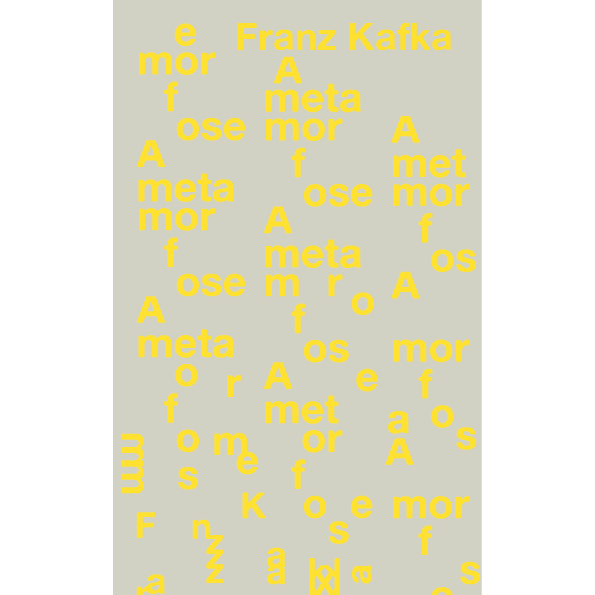
\includegraphics[width=92mm]{./grid/kafka.png}
\end{center}

\hspace*{-7cm}\hrulefill\hspace*{-7cm}

\medskip

\noindent{}Obra mais famosa de Franz Kafka, {\slsc{A metamorfose}} dispensa apresentações. A história da transformação de Gregor Samsa é um clássico porque condensa perfeitamente as características da prosa kafkiana, conceito que se torna importante na nossa repertoriação do mundo: kafkiano é, pois, o contraditório da cultura ocidental desumanizada, em que o irracional é criado justamente pelas estruturas burocráticas ultrarracionalizadas.

Samsa, o personagem principal, uma vez transformado em inseto, toma consciência de que sua alienação precedia a mutação de seu corpo. É a própria metamorfose que lhe dá a chance de olhar de si para si, sujeito e objeto. Franz Kafka é, pois, um realista, do único tipo que o século \scalebox{.8}{XX} comporta. O naturalismo do século \scalebox{.8}{XIX} não faz mais sentido no mundo em que o culto à razão produziu duas guerras mundiais; o caminho para o real é pela via do absurdo.

%\hspace{.5cm}
\vfill
\enlargethispage{\baselineskip}

\hspace*{-.4cm}\begin{minipage}[c]{.5\linewidth}
\small{
{\Formular{\textbf{
\hspace*{-.1cm}Título: A metamorfose [bilíngue]\\
Autor: Franz Kafka\\ 
ISBN: 978-85-7715-601-6\\
Páginas: 196\\
Formato: 13x21cm\\
Preço: R\$ 39,90\\
Editora: Hedra\\
Disponibilidade: 25/09/2020
}}}}
\end{minipage}


\pagebreak

\hspace{.5cm}

\begin{center}
\hspace*{.5cm}
\includegraphics[width=92mm]{./grid/maquiavel.jpg}
\end{center}

\hspace*{-7cm}\hrulefill\hspace*{-7cm}

\medskip

\noindent{}{\slsc{O príncipe}} ganha sua mais completa edição bilíngue, a partir da melhor publicação original italiana --- a Edição Crítica Inglese ---, acrescida de introdução e notas explicativas. Obra mais emblemática de Nicolau Maquiavel, {\slsc{O príncipe}} assinala nova forma de analisar a política, marcada pelo realismo que procura a apreender como ela é: em sua prática terrena. Se a intenção do autor é “escrever coisa útil”, seus conselhos para o príncipe não podem desconsiderar que “há tanta diferença entre como se vive e como se deveria viver, que quem deixa aquilo que se faz por aquilo que se deveria fazer apreende mais rapidamente a sua ruína que a sua preservação”.

É no espírito do realismo maquiaveliano que foram constituídos muitos dos enunciados polêmicos que fizeram a fama d'{\slsc{O príncipe}} e o tornaram um autor maldito, conhecido mais por estereótipos do que por seus escritos. Marco teórico e histórico, a obra é um clássico que preserva sua atualidade ao discorrer sobre a forma de governo de um mundo que, de muitas maneiras, ainda é o nosso.


\vfill

\hspace*{-.4cm}\begin{minipage}[c]{.5\linewidth}
\small{
{\Formular{\textbf{
\hspace*{-.1cm}Título: O príncipe [bilíngue]\\
Autor: Nicolau Maquiavel\\ 
ISBN: 978-85-7715-604-7\\
Páginas: 508\\
Formato: 13x21cm\\
Preço: R\$ 49,90\\
Editora: Hedra\\
Disponibilidade: 25/09/2020
}}}}
\end{minipage}



\pagebreak
\pagestyle{hedracat}

\begin{multicols}{2}
\begin{enumerate}
\item Ecopolítica, {\Formular{\textbf{Edson Passetti (org.)}}}	
\item Mare nostrum: Paranã Tipi, {\Formular{\textbf{Fabio Atui}}}
\item Crônicas de caça e criação, {\Formular{\textbf{Uirá Garcia}}}
\item Nas redes guarani, {\Formular{\textbf{Valéria Macedo}}}
\item A constituição traída, {\Formular{\textbf{Cleonildo Cruz (org.)}}}
\item Diário de um escritor na Rússia, {\Formular{\textbf{Flávio Ricardo Vassoler}}}
\item Lugar de negro, lugar de branco?, {\Formular{\textbf{Douglas Rodrigues Barros}}}
\item A sociedade de controle, {\Formular{\textbf{Sergio Amadeu (org.)}}}
\item O renascimento do autor, {\Formular{\textbf{Caio Gagliardi}}}
\item O que eu vi o que nós veremos, {\Formular{\textbf{Santos Dumont}}}
\item O outro lado da moeda (Teleny), {\Formular{\textbf{Oscar Wilde}}}
\item Imagens de um mundo trêmulo, {\Formular{\textbf{John Milton}}}
\item Michel Temer e o fascismo comum, {\Formular{\textbf{Tales Ab'Sáber}}}
\item Ao longo do rio, {\Formular{\textbf{Alexandre Koji Shiguehara}}}
\item Solombra, ou a sombra que cai sobre o eu, {\Formular{\textbf{João Adolfo Hansen}}}
\item Joana d'Arc, {\Formular{\textbf{Jules Michelet}}}
\item O coletivo aleatório, {\Formular{\textbf{Luis Marra}}}
\item A história das religiões na cultura moderna, {\Formular{\textbf{Marcello Massenzio}}}
\item Cordel - F. das Chagas Batista, {\Formular{\textbf{Francisco das Chagas Batista}}}
\item Elixir do pajé, {\Formular{\textbf{Bernardo Guimarães}}}
\item Cordel - João Martins de Athayde, {\Formular{\textbf{João Martins de Athayde}}}
\item Modos de representação da Bienal de São Paulo, {\Formular{\textbf{Vinicius Spricigo}}}
\item Padeirinho da Mangueira: retrato sincopado de um artista, {\Formular{\textbf{Franco Paulino}}}
\item Do futuro e da morte do teatro brasileiro, {\Formular{\textbf{Christina Barros Riego}}}
\item Canudos, história em versos, {\Formular{\textbf{Manuel Pedro das Dores Bombinho}}}
\item O cego e outros contos, {\Formular{\textbf{D. H. Lawrence}}}
\item Poesia seiscentista
\item Monoteísmos e dualismos: as religiões da salvação, {\Formular{\textbf{Giovanni Filoramo}}}
\item Apologia de Galileu, {\Formular{\textbf{Tommaso Campanella}}}
\item Flor do deserto, {\Formular{\textbf{Waris Dirie; Cathleen Miller}}}
\item Cinco lugares da fúria, {\Formular{\textbf{Pádua Fernandes}}}
\item O livro dos mandamentos, {\Formular{\textbf{Maimônides}}}
\item A conjuração de Catilina, {\Formular{\textbf{Salústio}}}
\item Fábula de Polifemo e Galatéia e outros poemas, {\Formular{\textbf{Góngora}}}
\item Histórias de igrejas destruídas, {\Formular{\textbf{Eduardo Brigagão Verderame}}}
\item Performances, {\Formular{\textbf{Brian Friel}}}
\item Cultura pop japonesa, {\Formular{\textbf{Sonia Bide Luyten}}}
\item História trágica do doutor Fausto, {\Formular{\textbf{Christopher Marlowe}}}
\item Micromegas, {\Formular{\textbf{Voltaire}}}
\item Politeísmos: as religiões do mundo antigo, {\Formular{\textbf{Paolo Scarpi}}}
\item Triunfos, {\Formular{\textbf{Petrarca}}}
\item Museu arte hoje, {\Formular{\textbf{Martin Grossmann; Gilberto Mariotti}}}
\item Viagem sentimental, {\Formular{\textbf{Laurence Sterne}}}
\item A Arte de olhar diferente, {\Formular{\textbf{Braulio Tavares}}}
\item O Pequeno Zacarias chamado Cinábrio, {\Formular{\textbf{E.T.A. Hoffman}}}
\item Oliver Twist (Bolso), {\Formular{\textbf{Charles Dickens}}}
\item Alegoria - Construção e interpretação da metáfora, {\Formular{\textbf{João Adolfo Hansen}}}
\item Teatro do êxtase, {\Formular{\textbf{Fernando Pessoa}}}
\item Paulo Whitaker, {\Formular{\textbf{Paulo Whitaker}}}
\item Todas as coisas pequenas, {\Formular{\textbf{Noemi Jaffe}}}
\item Questão do fim da arte em Hegel, {\Formular{\textbf{Marco Aurélio Werle}}}
\item Tratados da terra e gente do Brasil, {\Formular{\textbf{Fernão Cardim}}}
\item Dos nervos, {\Formular{\textbf{Ricardo Lísias}}}
\item Adeus ponta do meu nariz, {\Formular{\textbf{Edward Lear}}}
\item Cidade ampliada, {\Formular{\textbf{Rodrigo José Fermino}}}
\item O diário perdido do Jardim Maia, {\Formular{\textbf{Luís Marra}}}
\item Sobre a filosofia e outros diálogos, {\Formular{\textbf{Jorge Luis Borges; Osvaldo Ferrari}}}
\item Cordel: Franklin Maxado, {\Formular{\textbf{Franklin Maxado}}}
\item Dos novos sistemas na arte, {\Formular{\textbf{Kazimir Malievitch}}}
\item Cordel: Cuíca de Santo Amaro, {\Formular{\textbf{Cuíca de Santo Amaro}}}
\item Manual da destruição, {\Formular{\textbf{Alexandre Dal Farra}}}
\item A imprensa carnavalesca no Brasil, {\Formular{\textbf{José Ramos Tinhorão}}}
\item Índia e Extremo Oriente: via da libertação e da imortalidade, {\Formular{\textbf{Massimo Raveri}}}
\item Leitores e leituras de Clarice Lispector
\item Círculos de coca e fumaça, {\Formular{\textbf{Danilo Paiva Ramos}}}
\item Cordel: Severino José, {\Formular{\textbf{Severino José}}}
\item Escritório; O Espaço da Produção, {\Formular{\textbf{Claudio Silveira Amaral}}}
\item As minas de Salomão, {\Formular{\textbf{Rider Haggard}}}
\item Crédito à morte, {\Formular{\textbf{Anselm Jappe}}}
\item A cidade e as serras, {\Formular{\textbf{Eça de Queiroz}}}
\item Oliver Twist, {\Formular{\textbf{Charles Dickens}}}
\item Dao De Jing, {\Formular{\textbf{Lao Zi}}}
\item Sobre a amizade e outros diálogos, {\Formular{\textbf{Jorge Luis Borges; Osvaldo Ferrari}}}
\item Aqui tem coisa, {\Formular{\textbf{Patativa do Assaré}}}
\item Dicionário livre do santome-português, {\Formular{\textbf{Araújo \& Hagemeijer}}}
\item Aqui tem coisa, {\Formular{\textbf{Patativa do Assaré}}}
\item Imagem contemporânea I
\item Cordel - J. Borges, {\Formular{\textbf{José Francisco Borges}}}
\item Exato acidente, {\Formular{\textbf{Tony Monti}}}
\item Woyzeck, {\Formular{\textbf{George Buchner}}}
\item Autobiografia de um super-herói, {\Formular{\textbf{Alexandre Barbosa de Souza}}}
\item O menino da rosa, {\Formular{\textbf{Tony Monti}}}
\item Cordel - Rouxinol do Rinaré, {\Formular{\textbf{Rouxinol do Rinaré}}}
\item Imagem contemporânea II
\item História da província Santa Cruz, {\Formular{\textbf{Pero de Magalhães Gandavo}}}
\item Édipo Rei, {\Formular{\textbf{Sófocles}}}
\item Cordel - José Soares, {\Formular{\textbf{José Soares}}}
\item Greve contra a guerra, {\Formular{\textbf{Ricardo Lísias}}}
\item Cidade anônima, {\Formular{\textbf{Beatriz Furtado}}}
\item Primeiro de abril, {\Formular{\textbf{André Luiz Pinto}}}
\item Cordel: Oliveira de Panelas, {\Formular{\textbf{Oliveira de Panelas}}}
\item Fazendo Rizoma
\item Uma história do futebol, {\Formular{\textbf{Bill Murray}}}
\item Gangorra, {\Formular{\textbf{Regina Sawaya}}}
\item Poesia vaginal, {\Formular{\textbf{Glauco Mattoso}}}
\item Cultura popular - uma introdução, {\Formular{\textbf{Dominic Strinati}}}
\item Vocabulário de música pop, {\Formular{\textbf{Roy Shuker}}}
\item A invenção da pornografia, {\Formular{\textbf{Lynn Hunt}}}
\item Eu conheci Benny Moré
\item Deriva, {\Formular{\textbf{André Fernandes}}}
\item Fedro, {\Formular{\textbf{Platão}}}
\item Sobre os sonhos e outros diálogos, {\Formular{\textbf{Jorge Luis Borges; Osvaldo Ferrari}}}
\item O sapo voador, {\Formular{\textbf{Ademir Barbosa Jr.}}}
\item Arcana coelestia e Apocalipsis revelata, {\Formular{\textbf{Emanuel Swedenborg}}}
\item Letra de forma, {\Formular{\textbf{Laura Estelita Teixeira}}}
\item Os cães de que desistimos, {\Formular{\textbf{Chantal Castel}}}
\item Cordel - Téo Azevedo, {\Formular{\textbf{Téo Azevedo}}}
\item O que eu vi, o que nós veremos [bolso], {\Formular{\textbf{Santos Dumont}}}
\item A Fábrica de robôs, {\Formular{\textbf{Karel Tchápek}}}
\item Folhas de relva, {\Formular{\textbf{Walt Whitman}}}
\item Helio Piñon : Ideias e formas, {\Formular{\textbf{Pfeiffe, Helen; Ana Rosa}}}
\item O Rabi de Bacherach e três artigos sobre o ódio racial, {\Formular{\textbf{Heinrich Heine}}}
\item Refugiados de Idomeni, {\Formular{\textbf{Gabriel Bonis}}}
\item Visão de psicanálise, {\Formular{\textbf{Renato Bulcão}}}
\item Viagem em volta do meu quarto, {\Formular{\textbf{Xavier de Maistre}}}
\item Contos clássicos de vampiro, {\Formular{\textbf{Lord Byron; Bram Stoker}}}
\item Cultura estética e liberdade, {\Formular{\textbf{Friedrich Von Schiller}}}
\item Dostoiévski e a dialética, {\Formular{\textbf{Flávio Ricardo Vassoler}}}
\item Cabeças e outros poemas, {\Formular{\textbf{Pedro Luis Marques de Armas}}}
\item Razão sangrenta, {\Formular{\textbf{Robert Kurz}}}
\item A Velha Izerguil e outros contos, {\Formular{\textbf{Maksim Górki}}}
\item Viagem à turquia, bálcãs e Egito, {\Formular{\textbf{John Milton}}}
\item Do sentimento trágico da vida, {\Formular{\textbf{Miguel de Unamuno}}}
\item Rashômon e outros contos, {\Formular{\textbf{Akutagawa}}}
\item Feitiço de amor e outros contos, {\Formular{\textbf{Johann Ludwig Tieck}}}
\item Ode ao Vento Oeste e outros poemas, {\Formular{\textbf{P. B. Shelley}}}
\item Esperança do mundo, {\Formular{\textbf{Albert Camus}}}
\item Universidade, cidade, cidadania, {\Formular{\textbf{Franklin Leopoldo e Silva}}}
\item Estado crítico, {\Formular{\textbf{Régis Bonvicino}}}
\item Poemas da cabana montanhesa, {\Formular{\textbf{Saigyo}}}
\item Dançando em Lúnassa, {\Formular{\textbf{Brian Frield}}}
\item Lulismo, carisma pop e cultura anticrítica, {\Formular{\textbf{Tales Ab'Sáber}}}
\item Utopia Brasil, {\Formular{\textbf{Darcy Ribeiro}}}
\item Americanismo e fordismo, {\Formular{\textbf{Antonio Gramsci}}}
\item Troca de pele, {\Formular{\textbf{Tereza Yamashita}}}
\item O Surgimento da noite, {\Formular{\textbf{Pajés Parahiteri}}}
\item Contos de Sebastopol, {\Formular{\textbf{Liev Tolstói}}}
\item Um anarquista e outros contos, {\Formular{\textbf{Joseph Conrad}}}
\item Um Retrato do artista quando jovem, {\Formular{\textbf{James Joyce}}}
\item O Princípio do Estado e outros ensaios, {\Formular{\textbf{Mikhail Bakunin}}}
\item A Desmedida na medida, {\Formular{\textbf{Albert Camus}}}
\item O Chamado selvagem, {\Formular{\textbf{Jack London}}}
\item O Novo epicuro, {\Formular{\textbf{Edward Sellon}}}
\item Elogio da loucura, {\Formular{\textbf{Erasmo de Rotterdam}}}
\item Senhorita Júlia e outras peças, {\Formular{\textbf{August Strindberg}}}
\item Dublinenses, {\Formular{\textbf{James Joyce}}}
\item Don Juan ou O convidado de pedra, {\Formular{\textbf{Molière}}}
\item Manual inútil da televisão, {\Formular{\textbf{Paulo Henrique Amorim}}}
\item A Vida de Mat, {\Formular{\textbf{Mino Carta}}}
\item Baleiazzzul, {\Formular{\textbf{Sergio Zlotnic}}}
\item A Decadência do analfabetismo / A arte de birlibirloque, {\Formular{\textbf{José Bergamín}}}
\item Balada dos enforcados e outros poemas, {\Formular{\textbf{François Villon}}}
\item O Médico e o monstro, {\Formular{\textbf{Robert Louis Stevenson}}}
\item Marco Cornélio Frontão, {\Formular{\textbf{Pascal Quignard}}}
\item O Casamento do Céu e do Inferno, {\Formular{\textbf{William Blake}}}
\item O Homem da cabeça de papelão, {\Formular{\textbf{João do Rio}}}
\item Teleny, ou o reverso da medalha, {\Formular{\textbf{Oscar Wilde}}}
\item Cordel: Rodolfo Coelho Cavalcante, {\Formular{\textbf{Coelho Cavalcante}}}
\item Dicionário de História e Cultura da era Viking, {\Formular{\textbf{Johnni Langer}}}
\item Gente de Hemsö, {\Formular{\textbf{August Strindberg}}}
\item Viagem aos Estados Unidos, {\Formular{\textbf{Alexis de Tocqueville}}}
\item Sobre a utilidade e a desvantagem da história para a vida, {\Formular{\textbf{Friedrich Nietzsche}}}
\item Flossie, a Vênus de quinze anos, {\Formular{\textbf{Charles Swinburne}}}
\item Os cantos do homem-sombra
\item Escritos revolucionários, {\Formular{\textbf{Errico Malatesta}}}
\item Micromegas e outros contos, {\Formular{\textbf{Voltaire}}}
\item Descobrindo o Islã no Brasil, {\Formular{\textbf{Karla Lima}}}
\item A Cidade mágica, {\Formular{\textbf{Edith Nesbitt}}}
\item O Alienista, {\Formular{\textbf{Machado de Assis}}}
\item Cadeira de balanço, {\Formular{\textbf{Vanessa Campos Rocha; Flávio Castellan}}}
\item Inspiração nordestina, {\Formular{\textbf{Patativa do Assaré}}}
\item Coisas que a gente gosta e não gosta, {\Formular{\textbf{Laura Teixeira; Fábio Zimbres}}}
\item A Guerra começou, onde está a guerra?, {\Formular{\textbf{Albert Camus}}}
\item Poesia completa, {\Formular{\textbf{Orides Fontela}}}
\item A Volta do parafuso, {\Formular{\textbf{Henry James}}}
\item Cartas a favor da escravidão, {\Formular{\textbf{José de Alencar}}}
\item Pequeno-burgueses, {\Formular{\textbf{Maksim Górki}}}
\item Cordel : Paulo Nunes Batista, {\Formular{\textbf{Paulo Nunes Batista}}}
\item Esquimó, {\Formular{\textbf{Olivier Douzou}}}
\item Sai da frente, vaca brava!, {\Formular{\textbf{Ricardo Lísias}}}
\item Lampião... Era o cavalo do tempo atrás da besta da vida, {\Formular{\textbf{Antônio Klévisson Viana}}}
\item Cordel: Patativa do Assaré, {\Formular{\textbf{Patativa do Assaré}}}
\item Ernestine ou o nascimento do amor, {\Formular{\textbf{Stendhal}}}
\item Filadélfia, lá vou eu!, {\Formular{\textbf{Brian Friel}}}
\item Sonetos, {\Formular{\textbf{William Shakespeare}}}
\item Crônicas do crack, {\Formular{\textbf{Luis Marra}}}
\item Peixinhos, {\Formular{\textbf{Bruno Heitz}}}
\item A Última folha e outros contos, {\Formular{\textbf{O. Henry}}}
\item Contos indianos, {\Formular{\textbf{Stéphane Mallarmé}}}
\item Violência, mas para quê?, {\Formular{\textbf{Anselm Jappe}}}
\item A Vênus das peles, {\Formular{\textbf{Sacher-Leopold Von Masoch}}}
\item A Voz dos botequins e outros poemas, {\Formular{\textbf{Paul Verlaine}}}
\item Poemas, {\Formular{\textbf{Lord Byron}}}
\item A Pele do lobo e outras peças, {\Formular{\textbf{Artur Azevedo}}}
\item Explosão - Romance da etnologia, {\Formular{\textbf{Hubert Fichte}}}
\item Stephen herói, {\Formular{\textbf{James Joyce}}}
\item Diálogo imaginário entre Marx e Bakunin, {\Formular{\textbf{Maurice Cranston}}}
\item Nada ainda?, {\Formular{\textbf{Christian Voltz}}}
\item A Vênus de quinze anos (Flossie), {\Formular{\textbf{Charles Swinburne}}}
\item Os dentinhos, {\Formular{\textbf{Olivier Douzou}}}
\item Anarquismo, {\Formular{\textbf{Murray Bookchin}}}
\item Escritos sobre arte, {\Formular{\textbf{Charles Baudelaire}}}
\item Deus e o Estado, {\Formular{\textbf{Mikhail Bakunin}}}
\item Pintura e escrita do mundo flutuante, {\Formular{\textbf{Madalena Hashimoto Cordaro}}}
\item A Árvore dos cantos, {\Formular{\textbf{Pajés Parahiteri}}}
\item Poesia catalã - das origens à Guerra Civil
\item Sobre a filosofia e seu método, {\Formular{\textbf{Arthur Schopenhauer}}}
\item Pensamento político de Maquiavel, {\Formular{\textbf{Johann Fichte}}}
\item Sobre a ética, {\Formular{\textbf{Arthur Schopenhauer}}}
\item A Autobiografia do poeta-escravo, {\Formular{\textbf{Juan Francisco Manzano}}}
\item Cálcio, {\Formular{\textbf{Pádua Fernandes}}}
\item Bola de sebo e outros contos, {\Formular{\textbf{Guy de Maupassant}}}
\item Como gente grande, {\Formular{\textbf{Anouk Ricard}}}
\item O Cavalo de Ébano, {\Formular{\textbf{Richard Burton}}}
\item Nos cumes do desespero, {\Formular{\textbf{Emil Cioran}}}
\item A Vênus das peles [Bolso], {\Formular{\textbf{Leopold Von Sacher-Masoch}}}
\item Homo Pictor, {\Formular{\textbf{Christoph Wulf}}}
\item 1964
\item Desenganos da vida humana e outros poemas, {\Formular{\textbf{Gregório de Matos}}}
\item A Nostálgica e outros contos, {\Formular{\textbf{Aléxandros Papadiamántis}}}
\item Cântico dos Cânticos, {\Formular{\textbf{Salomão}}}
\item Os Sovietes traídos pelos bolcheviques, {\Formular{\textbf{Rudolf Rocker}}}
\item Autobiografia de uma pulga, {\Formular{\textbf{Stanislas de Rhodes}}}
\item Auto da barca do Inferno, {\Formular{\textbf{Gil Vicente}}}
\item A Monadologia e outros textos, {\Formular{\textbf{Gottfried Leibniz}}}
\item O Surgimento dos pássaros, {\Formular{\textbf{Pajés Parahiteri}}}
\item Contos de piratas, {\Formular{\textbf{Arthur Conan Doyle}}}
\item O Mundo ou tratado da luz, {\Formular{\textbf{René Descartes}}}
\item Manifesto comunista, {\Formular{\textbf{Karl Marx; Friedrich Engels}}}
\item Lira grega, {\Formular{\textbf{Giuliana Ragusa}}}
\item Poesia basca - das origens à Guerra Civil
\item Cordel: Klévisson Viana, {\Formular{\textbf{Klévisson Viana}}}
\item Discursos ímpios, {\Formular{\textbf{Marquês de Sade}}}
\item Cordel : Raimundo Santa Helena, {\Formular{\textbf{Raimundo Santa Helena}}}
\item Primeiro livro dos amores, {\Formular{\textbf{Ovídio}}}
\item Último reino, {\Formular{\textbf{Pascal Quignard}}}
\item Da arte de construir, {\Formular{\textbf{Leon Battista Alberti}}}
\item Frankenstein, {\Formular{\textbf{Mary Shelley}}}
\item Cordel : Zé Saldanha, {\Formular{\textbf{Zé Saldanha}}}
\item Dilma Rousseff e o ódio político, {\Formular{\textbf{Tales Ab'Sáber}}}
\item Saga dos Volsungos, {\Formular{\textbf{Anônimo}}}
\item Linear G, {\Formular{\textbf{Gilberto Mendonça Teles}}}
\item Educação e sociologia, {\Formular{\textbf{Émile Durkheim}}}
\item Histórias com dragões, príncipes e serpentes, {\Formular{\textbf{Vários}}}
\item História do boi misterioso, {\Formular{\textbf{Leandro Gomes de Barros; Irani Med}}}
\item Sobre verdade e mentira, {\Formular{\textbf{Friedrich Nietzsche}}}
\item Sermões 2, {\Formular{\textbf{Antônio Vieira}}}
\item Lisístrata, {\Formular{\textbf{Aristófanes}}}
\item Os Americanos, {\Formular{\textbf{Nathaniel Hawthorne; Edgar Allan Poe; Herman Melville}}}
\item O Sol não espera, {\Formular{\textbf{Marília Castello Branco}}}
\item O Fim do ciúme e outros contos, {\Formular{\textbf{Marcel Proust}}}
\item Álcoois, {\Formular{\textbf{Guillaume Apollinaire}}}
\item A História do planeta azul, {\Formular{\textbf{Andri Snaer Magnason}}}
\item Entre camponeses, {\Formular{\textbf{Errico Malatesta}}}
\item Ispinho e Fulô, {\Formular{\textbf{Patativa do Assaré}}}
\item Mais dia menos dia, a paixão, {\Formular{\textbf{Nelson de Oliveira}}}
\item Teogonia, {\Formular{\textbf{Hesíodo}}}
\item Ação e percepção nos processos educacionais do corpo em formação, {\Formular{\textbf{Cecília Noriko Ito Saito}}}
\item Amores e outras imagens, {\Formular{\textbf{Filóstrato}}}
\item O Fantástico reparador de feridas, {\Formular{\textbf{Brian Friel}}}
\item Mangá, {\Formular{\textbf{Sonia Bide Luyten}}}
\item Inferno, {\Formular{\textbf{August Strindberg}}}
\item Romanceiro cigano, {\Formular{\textbf{Sermões}}}
\item Sagas, {\Formular{\textbf{August Strindberg}}}
\item O Destino do erudito, {\Formular{\textbf{Johann Fichte}}}
\item Diários de Adão e Eva, {\Formular{\textbf{Mark Twain}}}
\item Habitar, {\Formular{\textbf{André Fernandes}}}
\item O Desertor, {\Formular{\textbf{Silva Alvarenga}}}
\item Os Vínculos, {\Formular{\textbf{Giordano Bruno}}}
\item O Estranho caso do Dr. Jekyll e Mr. Hyde, {\Formular{\textbf{Robert Louis Stevenson}}}
\item Sátiras, fábulas, aforismos e profecias, {\Formular{\textbf{Leonardo da Vinci}}}
\item Poesia espanhola - das origens à Guerra Civil
\item Hino a Afrodite e outros poemas, {\Formular{\textbf{Safo de Lesbos}}}
\item Revolução e liberdade, {\Formular{\textbf{Mikhail Bakunin}}}
\item Cartas do Brasil, {\Formular{\textbf{Antonio Vieira}}}
\item A Mulher que virou Tatu
\item Sermões 1, {\Formular{\textbf{Antônio Vieira}}}
\item Fé e saber, {\Formular{\textbf{G.W. Friedrich Hegel}}}
\item Negras tormentas, {\Formular{\textbf{Alexandre Samis}}}
\item Cordel: Manoel Caboclo, {\Formular{\textbf{Manoel Caboclo}}}
\item Graciliano Ramos e A Novidade, {\Formular{\textbf{Ieda Lebensztayn}}}
\item Emília Galotti, {\Formular{\textbf{Gotthold Ephraim Lessing}}}
\item Dao De Jing, {\Formular{\textbf{Lao Zi}}}
\item Histórias escondidas, {\Formular{\textbf{Odilon Moraes}}}
\item Noites egípcias e outros contos, {\Formular{\textbf{Aleksandr Púchikin}}}
\item Carmilla, a vampira de Karnstein, {\Formular{\textbf{Sheridan Le Fanu}}}
\item O desafio de Lula, {\Formular{\textbf{Mino Carta; Gianni Carta}}}
\item A Filosofia na era trágica dos gregos, {\Formular{\textbf{Friedrich Nietzsche}}}
\item O Que é bom, o que é ruim, {\Formular{\textbf{Vladimir Maiakóvski}}}
\item Em busca do Japão contemporâneo, {\Formular{\textbf{John Milton}}}
\item A Vida de H.P. Lovecraft, {\Formular{\textbf{S.T. Joshi}}}
\item A Demanda do Santo Graal, {\Formular{\textbf{Anônimo}}}
\item Trabalhos e os dias, {\Formular{\textbf{Hesíodo}}}
\item Mensagem, {\Formular{\textbf{Fernando Pessoa}}}
\item Ode sobre a melancolia e outros poemas, {\Formular{\textbf{John Keats}}}
\item O Corno de si próprio e outros contos, {\Formular{\textbf{Marquês de Sade}}}
\item Hawthorne e seus musgos, {\Formular{\textbf{Herman Melville}}}
\item Memórias de um menino judeu do Bom Retiro, {\Formular{\textbf{Victor Nussenzwieg}}}
\item No coração das trevas, {\Formular{\textbf{Joseph Conrad}}}
\item Émile e Sophie ou os solitários, {\Formular{\textbf{Jean-Jaqcques Rousseau}}}
\item Investigação sobre o entendimento humano, {\Formular{\textbf{David Hume}}}
\item Ideias de canário, {\Formular{\textbf{Machado de Assis}}}
\item Eu acuso! / O processo do capitão Dreyfus, {\Formular{\textbf{Émile Zola; Rui Barbosa}}}
\item O Livro dos dragões, {\Formular{\textbf{Ovídio}}}
\item As Bacantes, {\Formular{\textbf{Eurípides}}}
\item Contos clássicos de vampiro [Bolso], {\Formular{\textbf{Lord Byron; Bram Stoker}}}
\item Sobre a liberdade, {\Formular{\textbf{Stuart Mill}}}
\item Metamorfoses, {\Formular{\textbf{Ovídio}}}
\item O Primeiro Hamlet, {\Formular{\textbf{William Shakespeare}}}
\item O Corvo, {\Formular{\textbf{Claudio Weber Abramo}}}
\item A Vida é sonho, {\Formular{\textbf{Calderón de La Barca}}}
\item Eu, {\Formular{\textbf{Augusto dos Anjos}}}
\item Cordel: Zé Vicente, {\Formular{\textbf{Zé Vicente}}}
\item Escritos sobre literatura, {\Formular{\textbf{Sigmund Freud}}}
\item Dez poemas da vizinhança vazia, {\Formular{\textbf{Iuri Pereira}}}
\item Um gato Indiscreto e outros contos, {\Formular{\textbf{Saki}}}
\item Ciclovia, {\Formular{\textbf{Ulisses Garcez}}}
\item O Livro de Monelle, {\Formular{\textbf{Marcel Schwob}}}
\item A Fábrica de robôs [Bolso], {\Formular{\textbf{Karel Tchápek}}}
\item Oração aos moços, {\Formular{\textbf{Rui Barbosa}}}
\item A Metamorfose, {\Formular{\textbf{Franz Kafka}}}
\item História de Aladim e a lâmpada maravilhosa, {\Formular{\textbf{Patativa do Assaré}}}
\item Ninfas, {\Formular{\textbf{Giorgio Agamben}}}
\item O Ladrão honesto e outros contos, {\Formular{\textbf{Fiódor Dostoiévski}}}
\item O Enigma Orides, {\Formular{\textbf{Gustavo de Castro}}}
\item A Cruzada das crianças / Vidas imaginárias, {\Formular{\textbf{Marcel Schwob}}}
\item Sobre o riso e a loucura, {\Formular{\textbf{Hipócrates}}}
\item Notas sobre o anarquismo, {\Formular{\textbf{Noam Chomsky}}}
\item Mare Nostrum, {\Formular{\textbf{Fabio Atui}}}
\item Cordel: Expedito Sebastião Da Silva, {\Formular{\textbf{Expedito Sebastião}}}
\item Mistério na zona sul, {\Formular{\textbf{Roberto Barbato Junior}}}
\item Cordel: Zé Melancia, {\Formular{\textbf{Zé Melancia}}}
\item Lulismo, carisma pop e cultura anticrítica, {\Formular{\textbf{Tales Ab'Sáber}}}
\item Perversão, {\Formular{\textbf{Robert J. Stoller}}}
\item Poesia galega - das origens à Guerra Civil
\item Naqueles morros, depois da chuva, {\Formular{\textbf{Edival Lourenço}}}
\item Os Comedores de terra, {\Formular{\textbf{Pajés Parahiteri}}}
\item Ilíada, {\Formular{\textbf{Homero}}}
\item A Semente e a torre, {\Formular{\textbf{Leonardo da Vinci}}}
\item A Farsa de Inês Pereira, {\Formular{\textbf{Gil Vicente}}}
\item Cão, {\Formular{\textbf{Rafael Mantovani}}}
\item Diário de um escritor (1873), {\Formular{\textbf{Fiódor Dostoiévski}}}
\item Carta sobre a tolerância, {\Formular{\textbf{John Locke}}}
\item Anarquia pela educação, {\Formular{\textbf{Élisée Reclus}}}
\item A Raposa sombria, {\Formular{\textbf{Sjón}}}
\item Anjos do universo, {\Formular{\textbf{Einar Már Gudmundsson}}}
\item O Indivíduo, a sociedade e o Estado e outros ensaios, {\Formular{\textbf{Emma Goldman}}}
\item A terra uma só, {\Formular{\textbf{Timóteo da Silva Verá Tupã Popyguá}}}
\item Mistério no morro do deleite, {\Formular{\textbf{Roberto Barbato Junior}}}
\item A arte de contar histórias, {\Formular{\textbf{Water Benjamin}}}
\end{enumerate}
\end{multicols}

\pagebreak